\documentclass[11pt,a4paper]{article}

% -----------------------------------------------------------------------------
% Packages
% -----------------------------------------------------------------------------
\usepackage[margin=2.5cm]{geometry}
\usepackage[T1]{fontenc}
\usepackage[utf8]{inputenc}
\usepackage{lmodern}
\usepackage{microtype}
\usepackage{graphicx}
\usepackage{booktabs}
\usepackage{array}
\usepackage{amsmath}
\usepackage{amssymb}
\usepackage{siunitx}
\usepackage{xcolor}
\usepackage{enumitem}
\usepackage{listings}
\usepackage{caption}
\usepackage{subcaption}
\usepackage{fancyhdr}
\usepackage[hidelinks]{hyperref}

% -----------------------------------------------------------------------------
% Document metadata and formatting
% -----------------------------------------------------------------------------
\newcommand{\reporttitle}{Patient-Specific Computational Fluid Dynamics of the Airways}
\newcommand{\reportsubtitle}{Segmentation, Mesh Generation, and Flow Analysis in Tracheomalacia}
\newcommand{\reportauthor}{Henri Van Overmeire}
\newcommand{\reportdate}{\today}

\definecolor{codebackground}{RGB}{245,247,250}
\definecolor{codekeyword}{RGB}{30,80,150}
\definecolor{codecomment}{RGB}{65,120,75}

\lstset{
  basicstyle=\ttfamily\small,
  backgroundcolor=\color{codebackground},
  keywordstyle=\color{codekeyword}\bfseries,
  commentstyle=\color{codecomment},
  frame=single,
  breaklines=true,
  columns=fullflexible,
  keepspaces=true,
  showstringspaces=false
}

\pagestyle{fancy}
\fancyhf{}
\fancyhead[L]{Airway CFD}
\fancyhead[R]{Henri Van Overmeire}
\fancyfoot[C]{\thepage}
\setlength{\headheight}{14pt}

\sisetup{
  detect-all,
  per-mode=symbol
}

\graphicspath{{figures/}}

\begin{document}
\hypersetup{pageanchor=false}

% -----------------------------------------------------------------------------
% Title page
% -----------------------------------------------------------------------------
\begin{titlepage}
  \centering
  \vspace*{2.5cm}

  {\Large Computational Biofluid Mechanics\par}
  \vspace{1.5cm}

  {\Huge\bfseries \reporttitle\par}
  \vspace{0.6cm}
  {\Large \reportsubtitle\par}

  \vfill

  \begin{tabular}{rl}
    \textbf{Author:} & \reportauthor \\
    \textbf{Date:}   & \reportdate \\
    \textbf{Repository:} &
    \href{https://github.com/henrivanovermeire/tracheomalacia_cfd/settings}
    {\texttt{github.com/henrivanovermeire/tracheomalacia\_cfd}}
  \end{tabular}

  \vfill

  \textit{Reproducible project report; analyses still in progress are identified
  explicitly in the text.}
\end{titlepage}

\hypersetup{pageanchor=true}
\pagenumbering{roman}

% -----------------------------------------------------------------------------
% Front matter
% -----------------------------------------------------------------------------
\begin{abstract}
Tracheomalacia is characterised by excessive collapse or narrowing of the
tracheal lumen and can substantially alter respiratory airflow. This project
uses patient-specific computed tomography, three-dimensional airway
segmentation, and computational fluid dynamics (CFD) to compare airflow before
and after intervention. Airway surfaces are segmented in 3D Slicer, clipped
along VMTK-derived centerlines, extended in the local centerline direction, and
closed with planar caps. Tetrahedral volume meshes are generated with Gmsh and
steady incompressible airflow is solved using OpenFOAM. This report documents
the reproducible processing pipeline, evaluates mesh quality and mesh
independence, and compares clinically relevant flow quantities between the
preoperative and postoperative geometries. The preoperative minimum lumen area
was \SI{1.813}{\milli\metre\squared}, compared with
\SI{5.169}{\milli\metre\squared} at the matched postoperative location, giving
an area constriction of 64.9\%. In the steady postoperative model the local
pressure drop was \SI{30.95}{\pascal}, the resistance was
\SI{15.41}{\pascal\per\litre\per\minute}, and 73.2\% of outlet flow entered the
right lung. A four-level HXT mesh study selected the \num{0.15}~mm mesh because
its reported metrics differed by no more than 2.02\% from the denser mesh while
using 48\% fewer cells. A complete-cycle transient calculation is configured;
its final phase-resolved results are reported only after solver completion.
\end{abstract}

\tableofcontents
\listoffigures
\listoftables
\clearpage
\pagenumbering{arabic}

% -----------------------------------------------------------------------------
\section{Introduction}
\label{sec:introduction}

Tracheomalacia involves reduced structural stability of the tracheal wall,
which may cause dynamic narrowing and increased respiratory resistance. While
medical imaging describes airway anatomy, CFD can quantify how geometric
narrowing influences velocity, pressure loss, flow distribution, and local
shear-related quantities.

The objectives of this project are to:

\begin{enumerate}[label=\arabic*.]
  \item construct patient-specific preoperative and postoperative airway
        geometries from computed tomography;
  \item establish a reproducible segmentation-to-simulation workflow;
  \item quantify airflow and pressure differences between the two cases; and
  \item assess whether the numerical conclusions are independent of mesh
        resolution.
\end{enumerate}

\subsection{Research questions}

\begin{itemize}
  \item How does the intervention change the minimum airway cross-section?
  \item How does the pressure drop across the trachea change?
  \item Where do peak velocities and recirculation regions occur?
  \item How is flow divided among the distal outlets?
  \item Are the reported quantities sufficiently mesh independent?
\end{itemize}

% -----------------------------------------------------------------------------
\section{Critical review of a selected CFD paper}
\label{sec:paper_review}

The selected paper is Taherian et al.'s patient-specific CFD evaluation of
excessive dynamic airway collapse before and after tracheal stenting
\cite{taherian2017}. Each of the five required subsections below is shorter than
150 words. No paper figures are reproduced, remaining within the permitted
maximum of three.

\subsection{Goal}

The study investigated whether patient-specific computational fluid dynamics
could quantify the functional consequences of excessive dynamic airway collapse
and assess improvement after tracheal stenting. The authors specifically
compared inspiratory and expiratory airflow before and after intervention using
CT-derived airway geometries. They aimed to determine how stenting affected
pressure loss, velocity, wall shear stress, and turbulence, and whether these
CFD quantities revealed clinically relevant changes that conventional pulmonary
function tests might miss. The underlying question was therefore not merely
whether the airway lumen became larger, but whether the anatomical intervention
produced a meaningful improvement in respiratory flow behaviour.

\subsection{Methods}

Four patient-specific airway models represented inspiration and expiration
before and after stenting. CT images were segmented in Mimics and simulated in
STAR-CCM+. Each rigid model included the trachea and approximately six to eight
airway generations. The authors simulated 2.5~s inspiration and 2.5~s expiration
with sinusoidal resting-breathing flow. Patient-specific outlet pressure
functions were derived in a preliminary step from lobar volume changes, while
the inlet was atmospheric with 10\% turbulence intensity. Unsteady RANS with a
low-Reynolds-number $k$--$\omega$ model and second-order spatial and temporal
schemes was used. Inlet and outlet extensions measured one and four hydraulic
diameters, respectively. Polyhedral meshes with prism layers were tested at
0.9, 1.7, and 3.2 million cells; 1.7 million cells was selected from pressure,
velocity, and wall-shear-stress sensitivity.

\subsection{Results}

Stenting produced the clearest improvement during expiration. The severe
pre-stent narrowing generated a high-velocity jet, recirculation, substantial
pressure loss, and elevated wall shear stress. The reported pre-/post-stent
expiratory pressure difference was approximately $26~\mathrm{cmH_2O}$, while
mean tracheal wall shear stress decreased from 3.98 to 0.793~Pa, an approximately
80\% reduction. Velocity variations also became smaller after stenting.
Inspiratory changes were comparatively minor; mean wall shear stress increased
from 0.0354 to 0.0813~Pa, and the stent introduced some local flow disturbance.
Turbulence intensity increased in parts of both phases after intervention.
Spirometry changed only modestly---FEV$_1$ increased by 290~mL---whereas CFD
exposed pronounced expiratory functional improvement that pulmonary function
testing did not clearly reflect.

\subsection{Limitations}

The study considered only one patient, so its quantitative findings cannot be
generalised to all patients with excessive dynamic airway collapse. The airway
walls were rigid even though wall deformation is the defining feature of the
disease. Separate end-inspiration and end-expiration geometries represented the
extremes of breathing rather than continuously moving anatomy; fluid--structure
interaction was omitted because patient-specific tissue properties were
unavailable. The upper airway and deeper peripheral generations were truncated,
although both may influence tracheal flow and outlet impedance. Outlet pressures
were inferred indirectly from lobar volume changes, and local CFD predictions
were not validated against invasive pressure or velocity measurements. The RANS
turbulence model and selected boundary conditions add model-form uncertainty.
Finally, mesh sensitivity was demonstrated primarily for selected quantities in
one pre-stent expiratory geometry.

\subsection{Evaluation}

For this patient, the authors largely answered their research question. The
paired pre-/post-stent and inspiration/expiration design isolated the phase in
which airway collapse mattered most, and pressure, velocity, and wall shear
stress changed coherently after intervention. The contrast with relatively
insensitive spirometry supports the claim that CFD can provide additional
functional information. The mesh test and patient-informed outlet conditions
strengthen the internal comparison. However, the study establishes a
patient-specific proof of concept rather than a validated diagnostic or
prognostic method. Rigid endpoint geometries cannot reproduce dynamic coupling
between airflow and collapse, and a single case cannot establish clinical
accuracy or treatment thresholds. Thus, the conclusion that stenting improved
this patient's expiratory airflow is supported, whereas broader claims about
CFD-guided management require validation in more patients with dynamic or
fluid--structure-interaction models.

% -----------------------------------------------------------------------------
\section{Imaging data and anatomical cases}
\label{sec:data}

Two computed-tomography datasets are analysed: a preoperative case and a
postoperative case. Table~\ref{tab:imaging} should be completed from the DICOM
metadata and segmentation logs.

\begin{table}[htbp]
  \centering
  \caption{Imaging and anatomical case information.}
  \label{tab:imaging}
  \begin{tabular}{@{}llll@{}}
    \toprule
    Case & Voxel dimensions & Voxel spacing (mm) & Clinical state \\
    \midrule
    Preoperative  & [insert] & [insert] & Before intervention \\
    Postoperative & [insert] & [insert] & After intervention \\
    \bottomrule
  \end{tabular}
\end{table}

All patient-derived data must be handled according to the applicable privacy,
ethics, and data-management requirements. No directly identifying information
should appear in this report or repository.

% -----------------------------------------------------------------------------
\section{Airway segmentation and surface preparation}
\label{sec:segmentation}

\subsection{Segmentation}

The CT series is loaded into 3D Slicer. A case-specific seed is placed in the
airway lumen, and connected region growth is performed within a selected
Hounsfield-unit interval. Thresholds and seed coordinates are stored under
\texttt{segmentation/assets/<case>/}. The result is inspected in axial,
coronal, sagittal, and three-dimensional views to exclude lung parenchyma and
external air while retaining the clinically relevant branches.

Record the final settings in Table~\ref{tab:segmentation}.

\begin{table}[htbp]
  \centering
  \caption{Final segmentation settings.}
  \label{tab:segmentation}
  \begin{tabular}{@{}llll@{}}
    \toprule
    Case & Lower HU & Upper HU & Segmented voxels \\
    \midrule
    Preoperative  & [insert] & [insert] & [insert] \\
    Postoperative & [insert] & [insert] & [insert] \\
    \bottomrule
  \end{tabular}
\end{table}

\subsection{Centerline extraction and clipping}

A centerline network is calculated using VMTK. Visually refined clipping points
are loaded as the Slicer markup node \texttt{AirwayCutEndpoints}. The airway is
clipped using the same \textit{Clip Vessel} logic as the SlicerVMTK user
interface, with \texttt{AirwayNetworkModel} providing the centerline direction.

Flow extensions are aligned with the local centerline and adapt to the airway
radius at each clipping location. Planar caps close the extensions for CFD. The
final Slicer model is \texttt{AirwayExtendedSurfaceCapped} and is exported as
\texttt{meshes/<case>/airways.stl}, preventing the two anatomies from
silently overwriting one another.

\begin{figure}[htbp]
  \centering
  \begin{subfigure}[t]{0.48\textwidth}
    \centering
    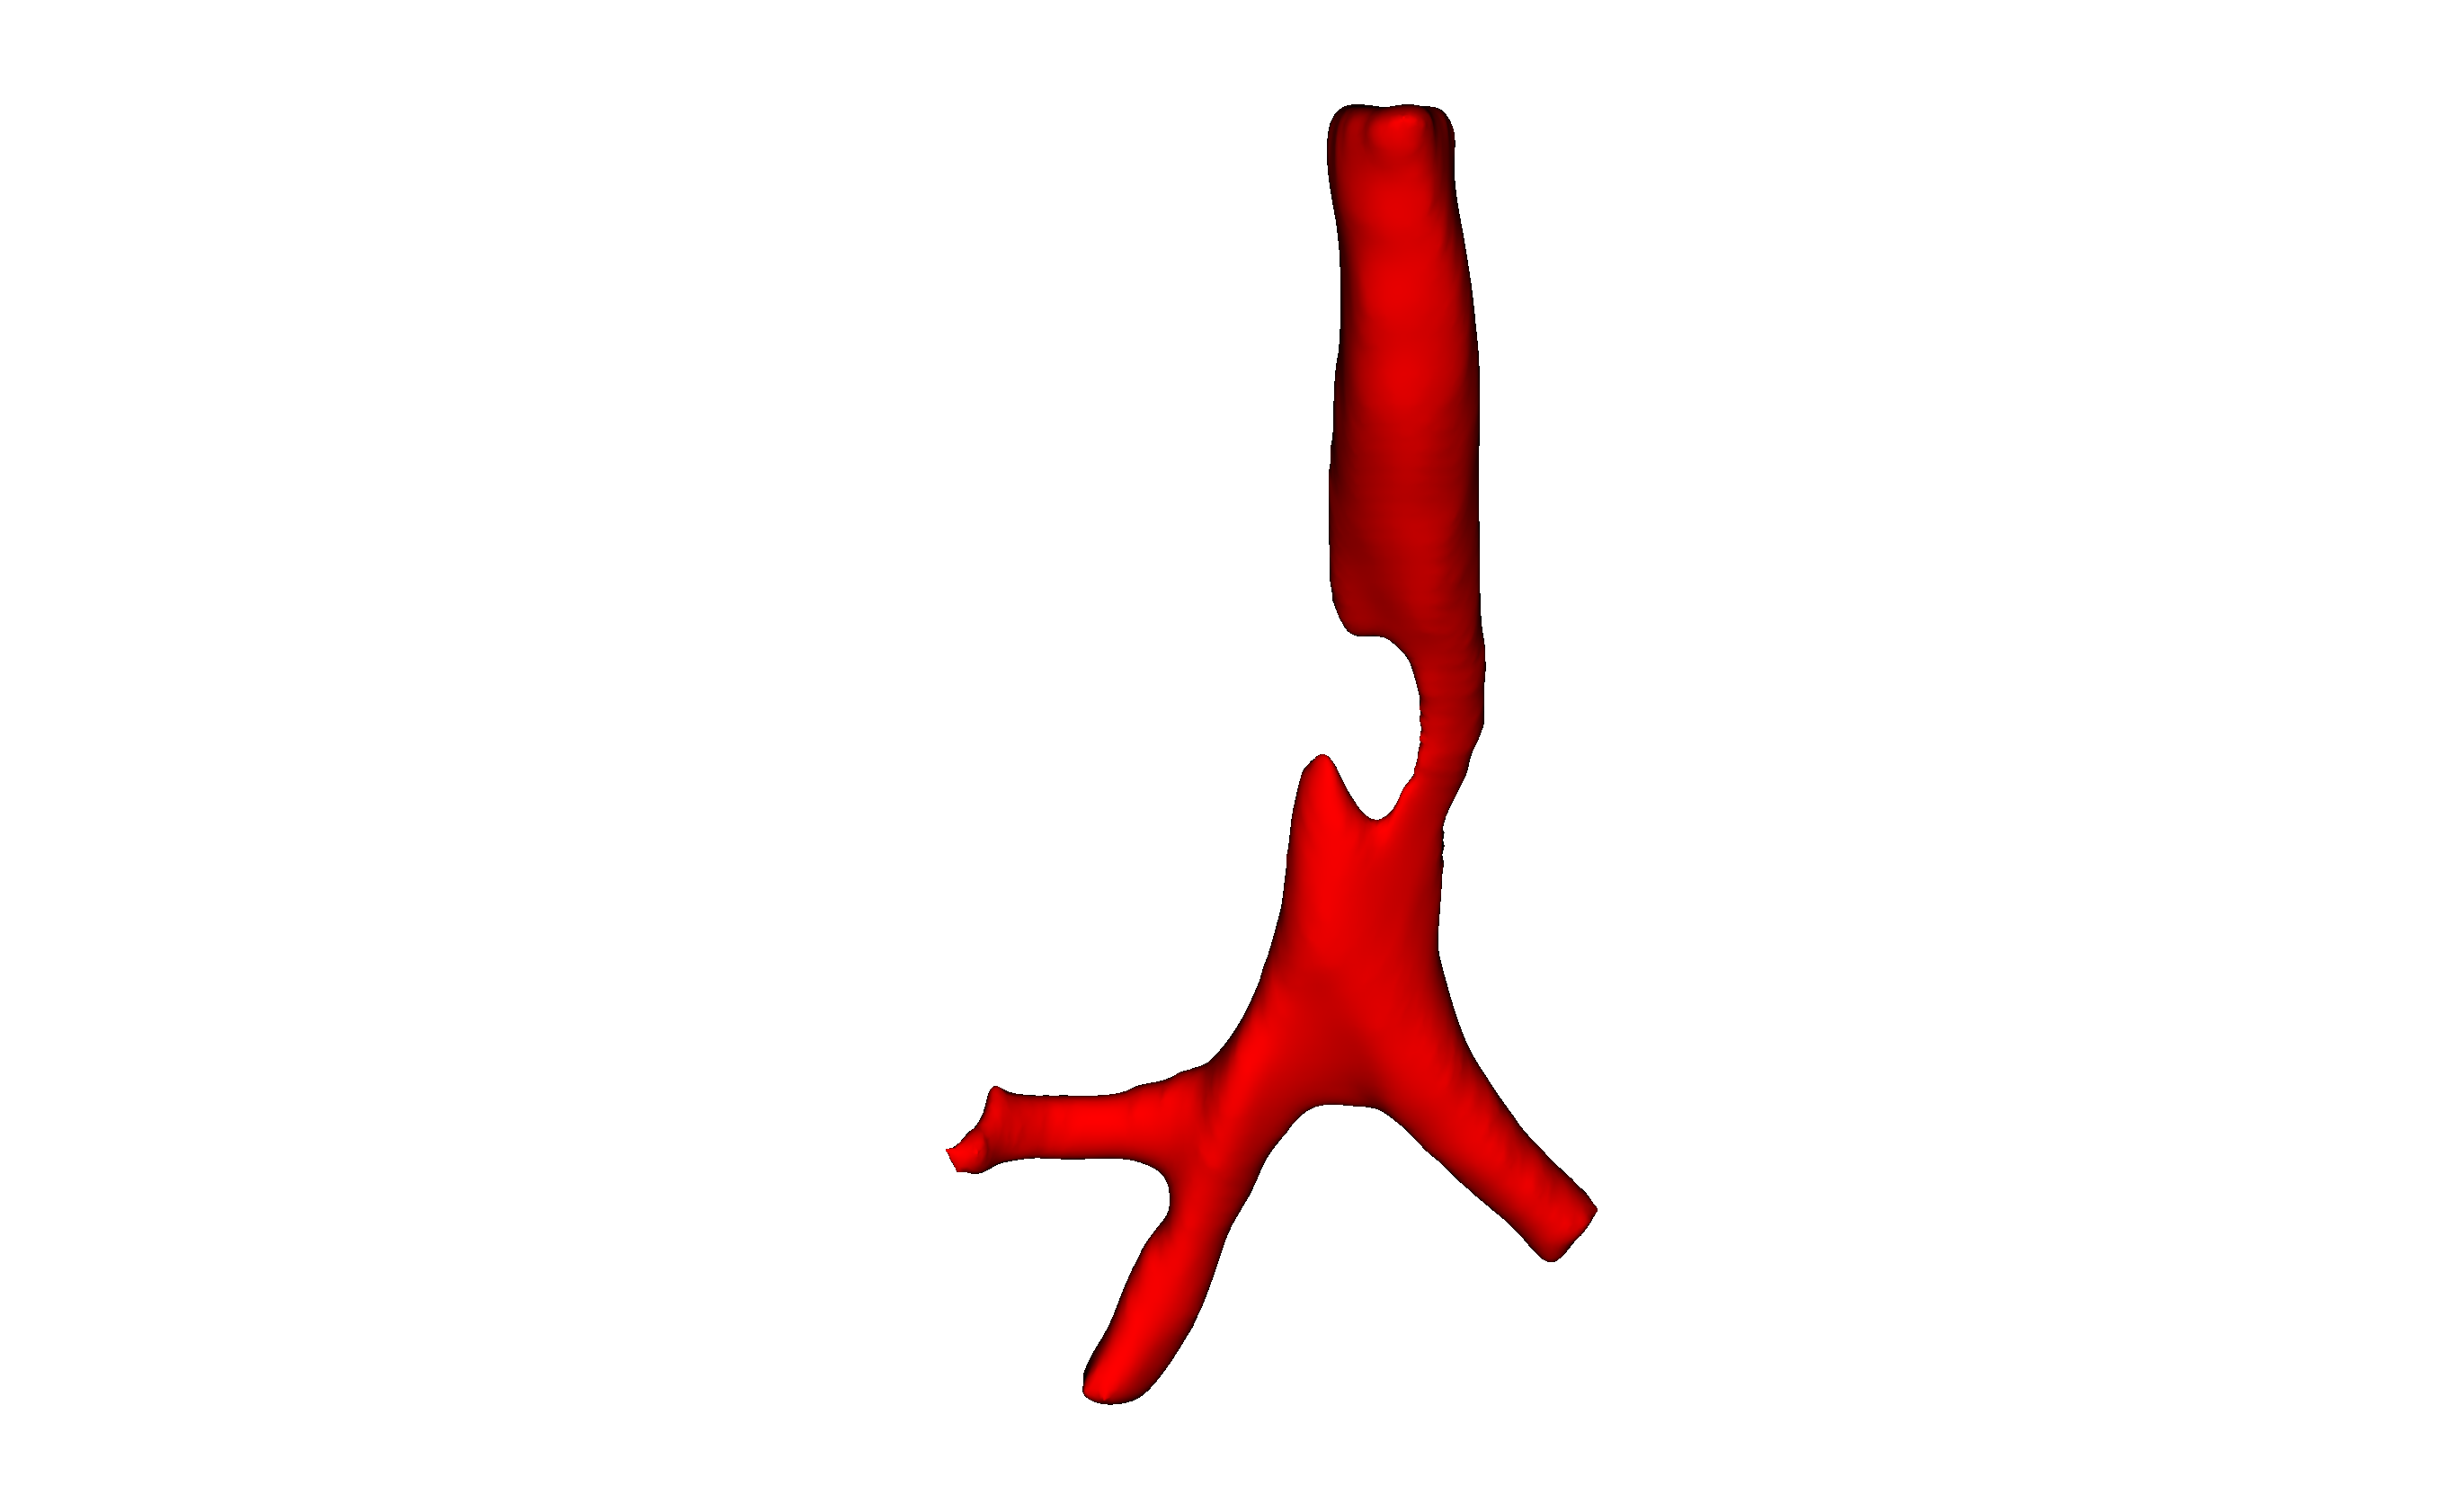
\includegraphics[width=\linewidth]{preop_segmentation.png}
    \caption{Preoperative cleaned airway segmentation.}
  \end{subfigure}\hfill
  \begin{subfigure}[t]{0.48\textwidth}
    \centering
    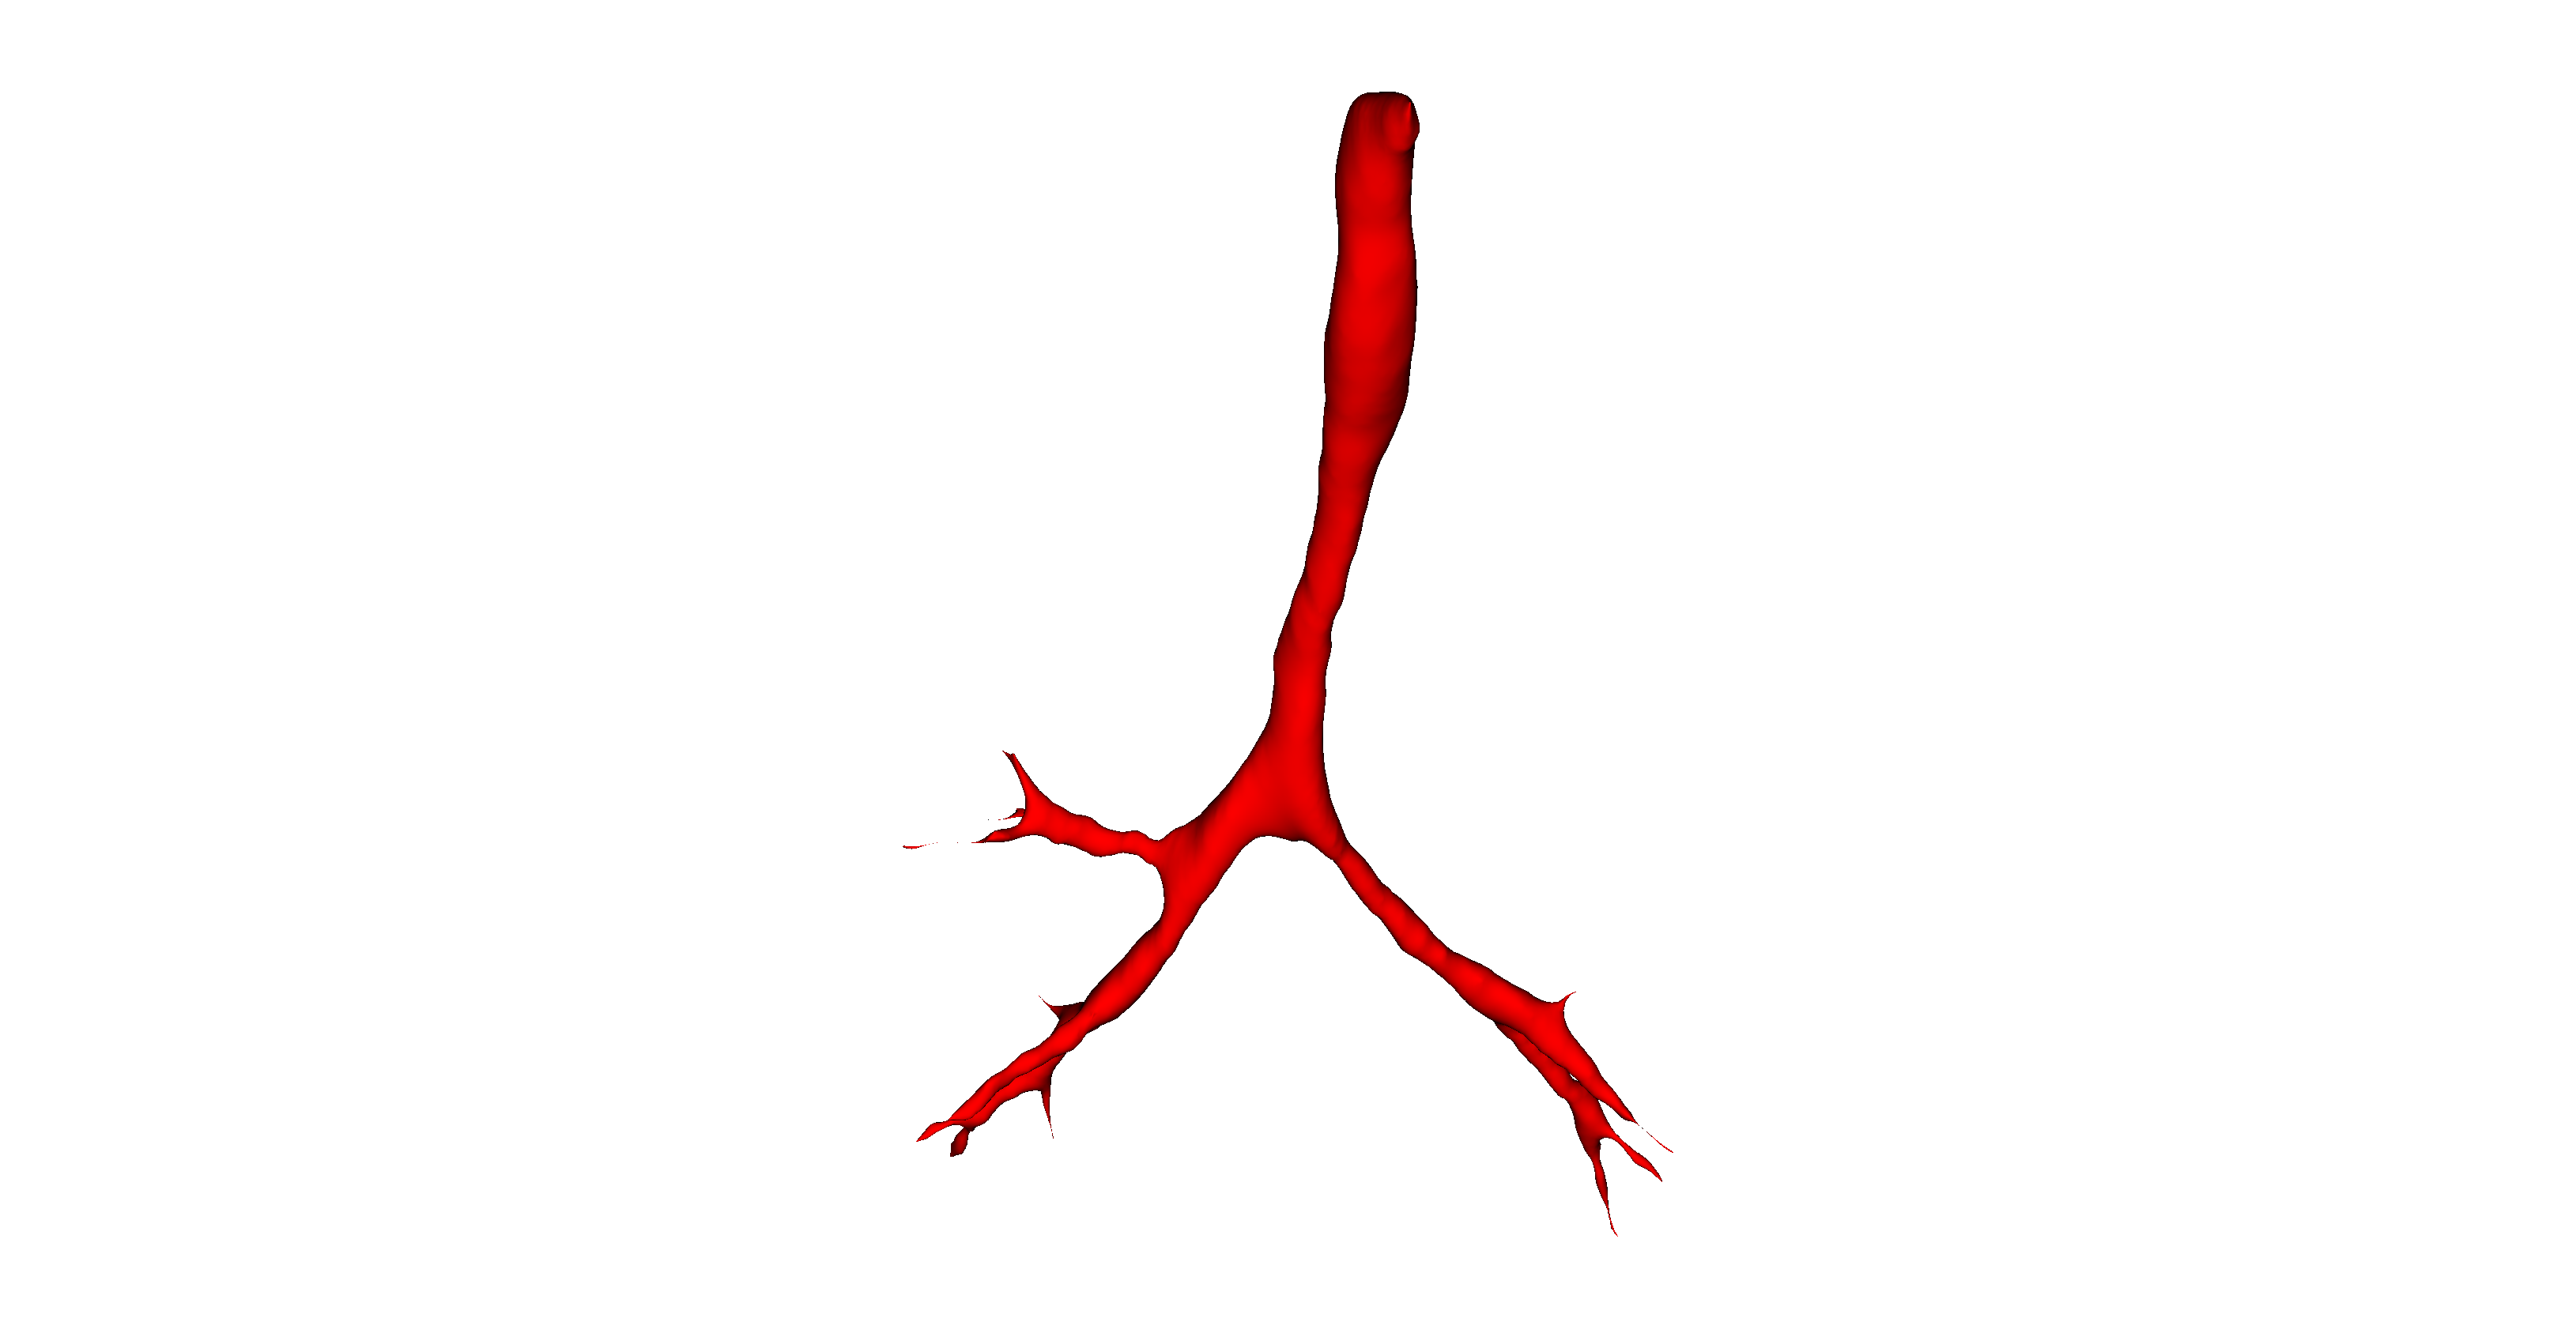
\includegraphics[width=\linewidth]{postop_segmentation.png}
    \caption{Postoperative airway segmentation.}
  \end{subfigure}

  \vspace{0.5em}
  \begin{subfigure}[t]{0.48\textwidth}
    \centering
    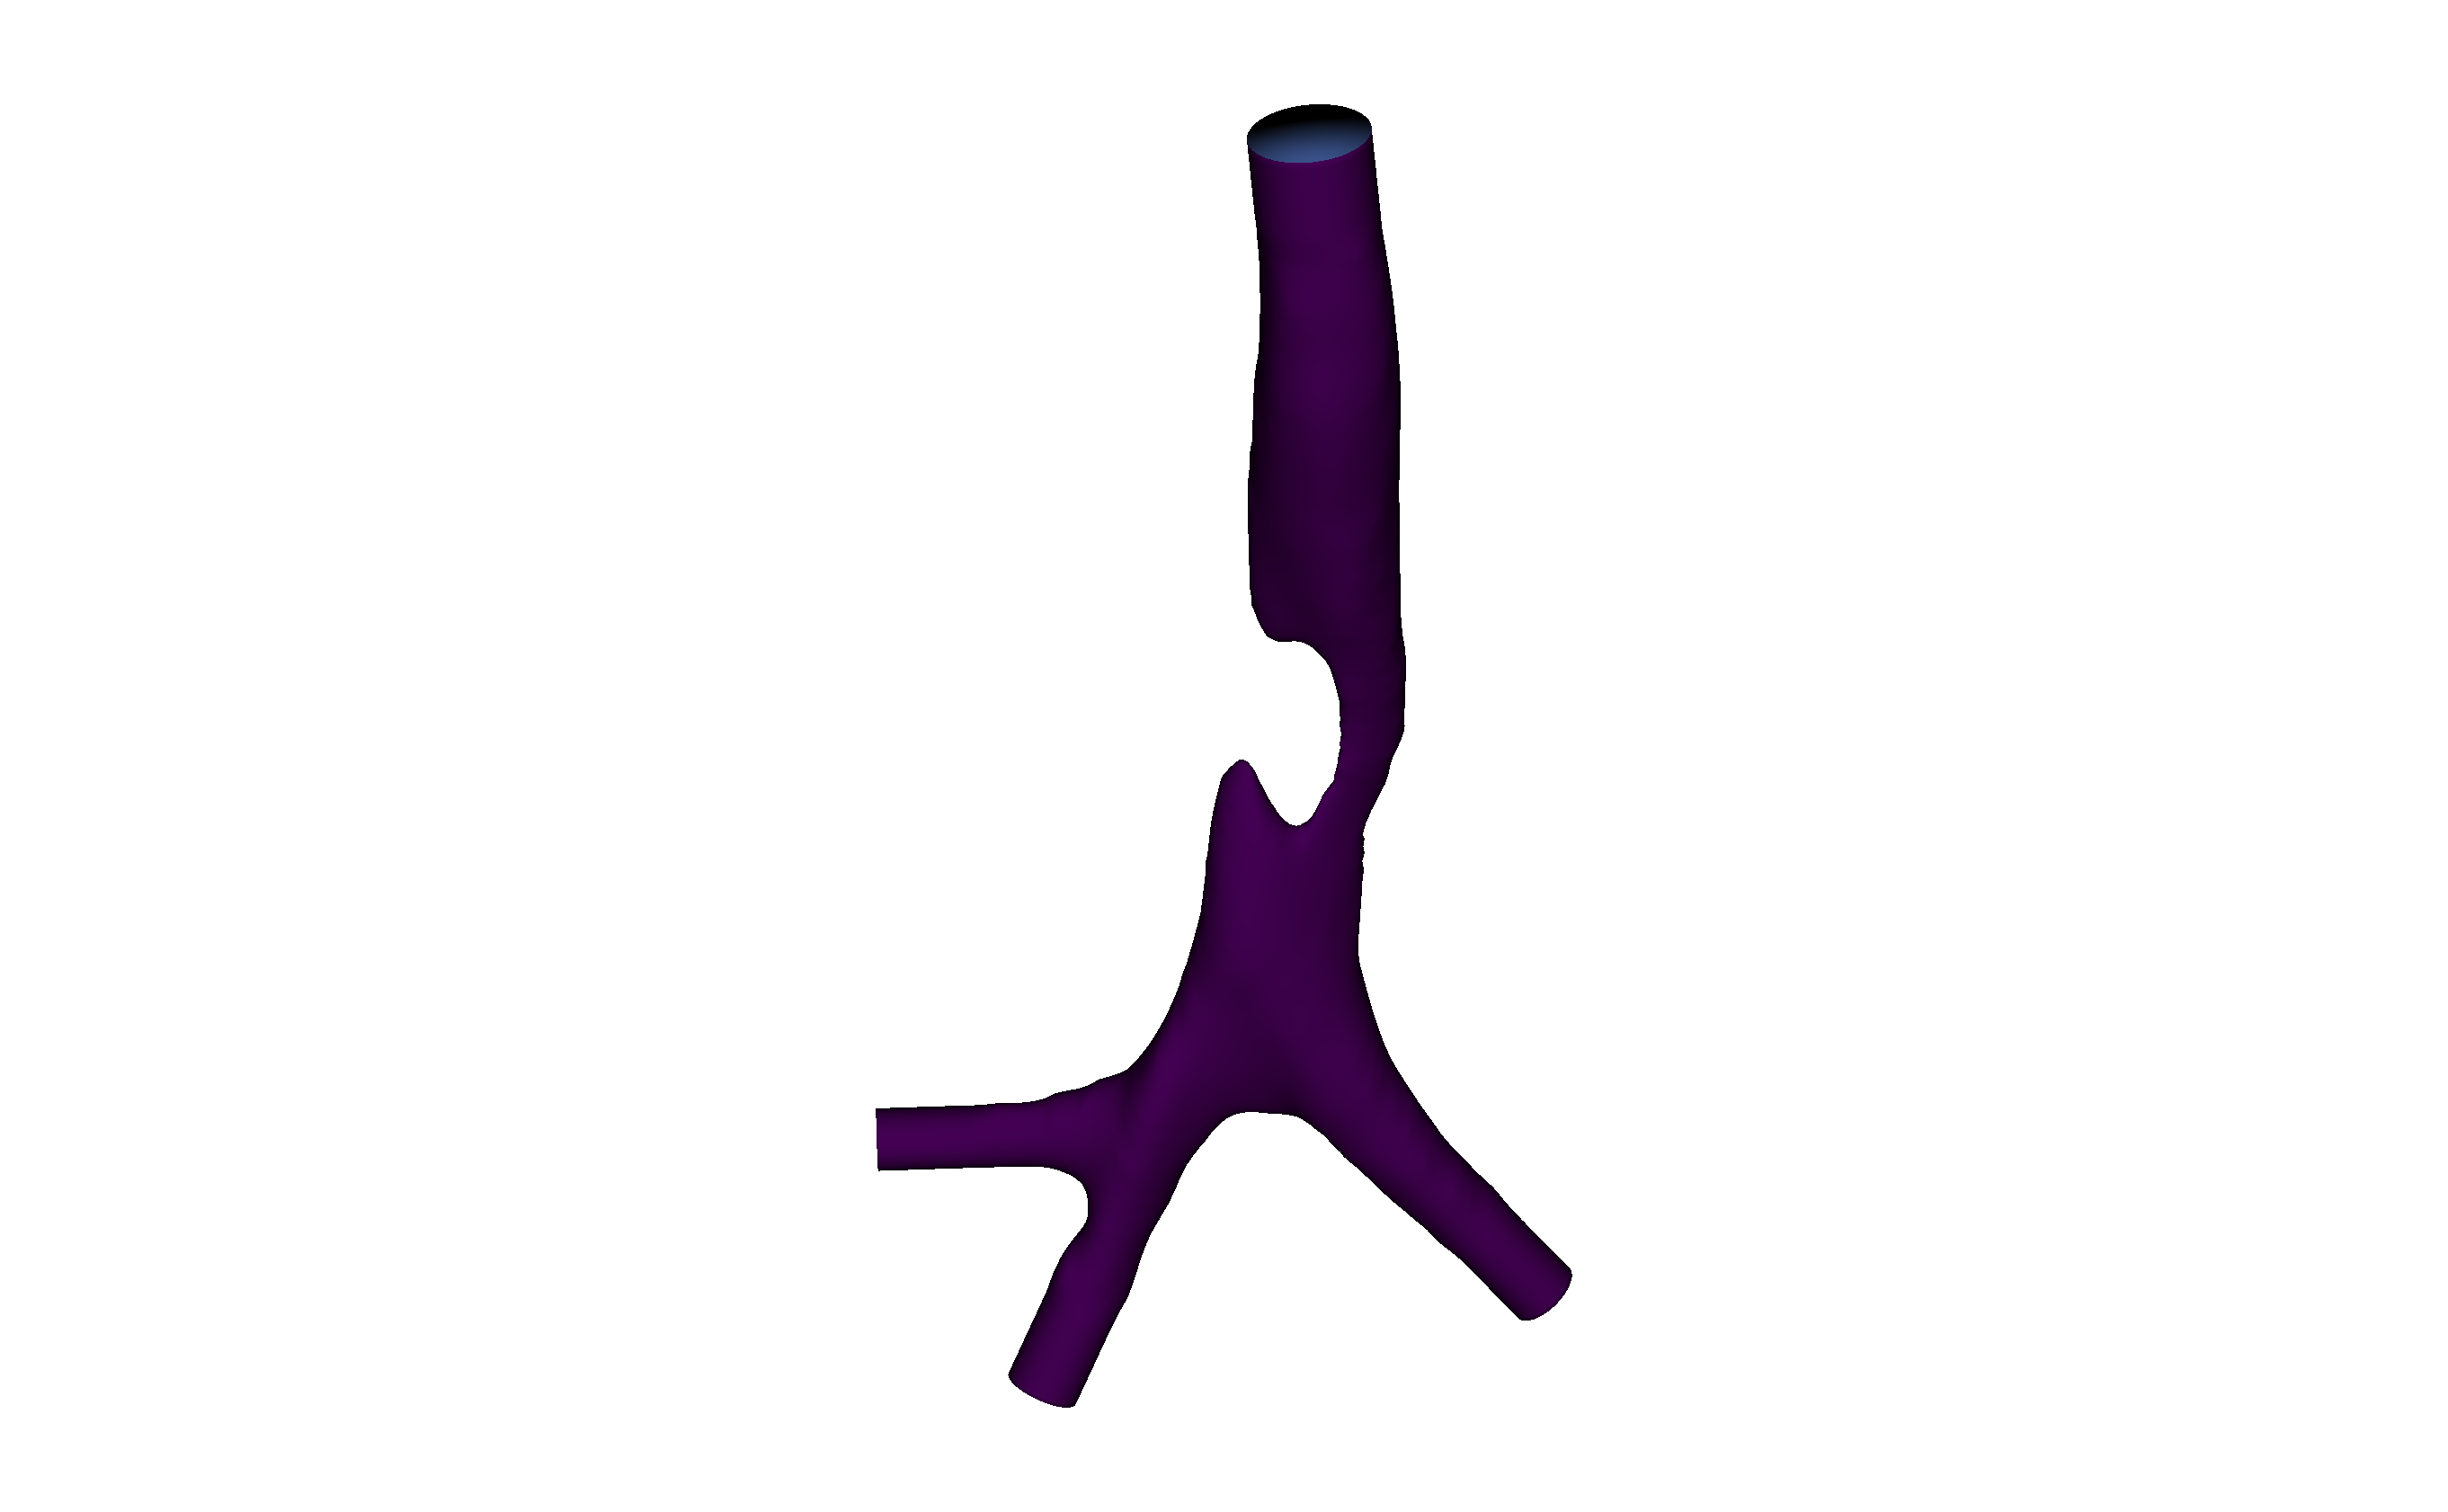
\includegraphics[width=\linewidth]{preop_cfd_surface.png}
    \caption{Preoperative clipped, extended, and capped surface.}
  \end{subfigure}\hfill
  \begin{subfigure}[t]{0.48\textwidth}
    \centering
    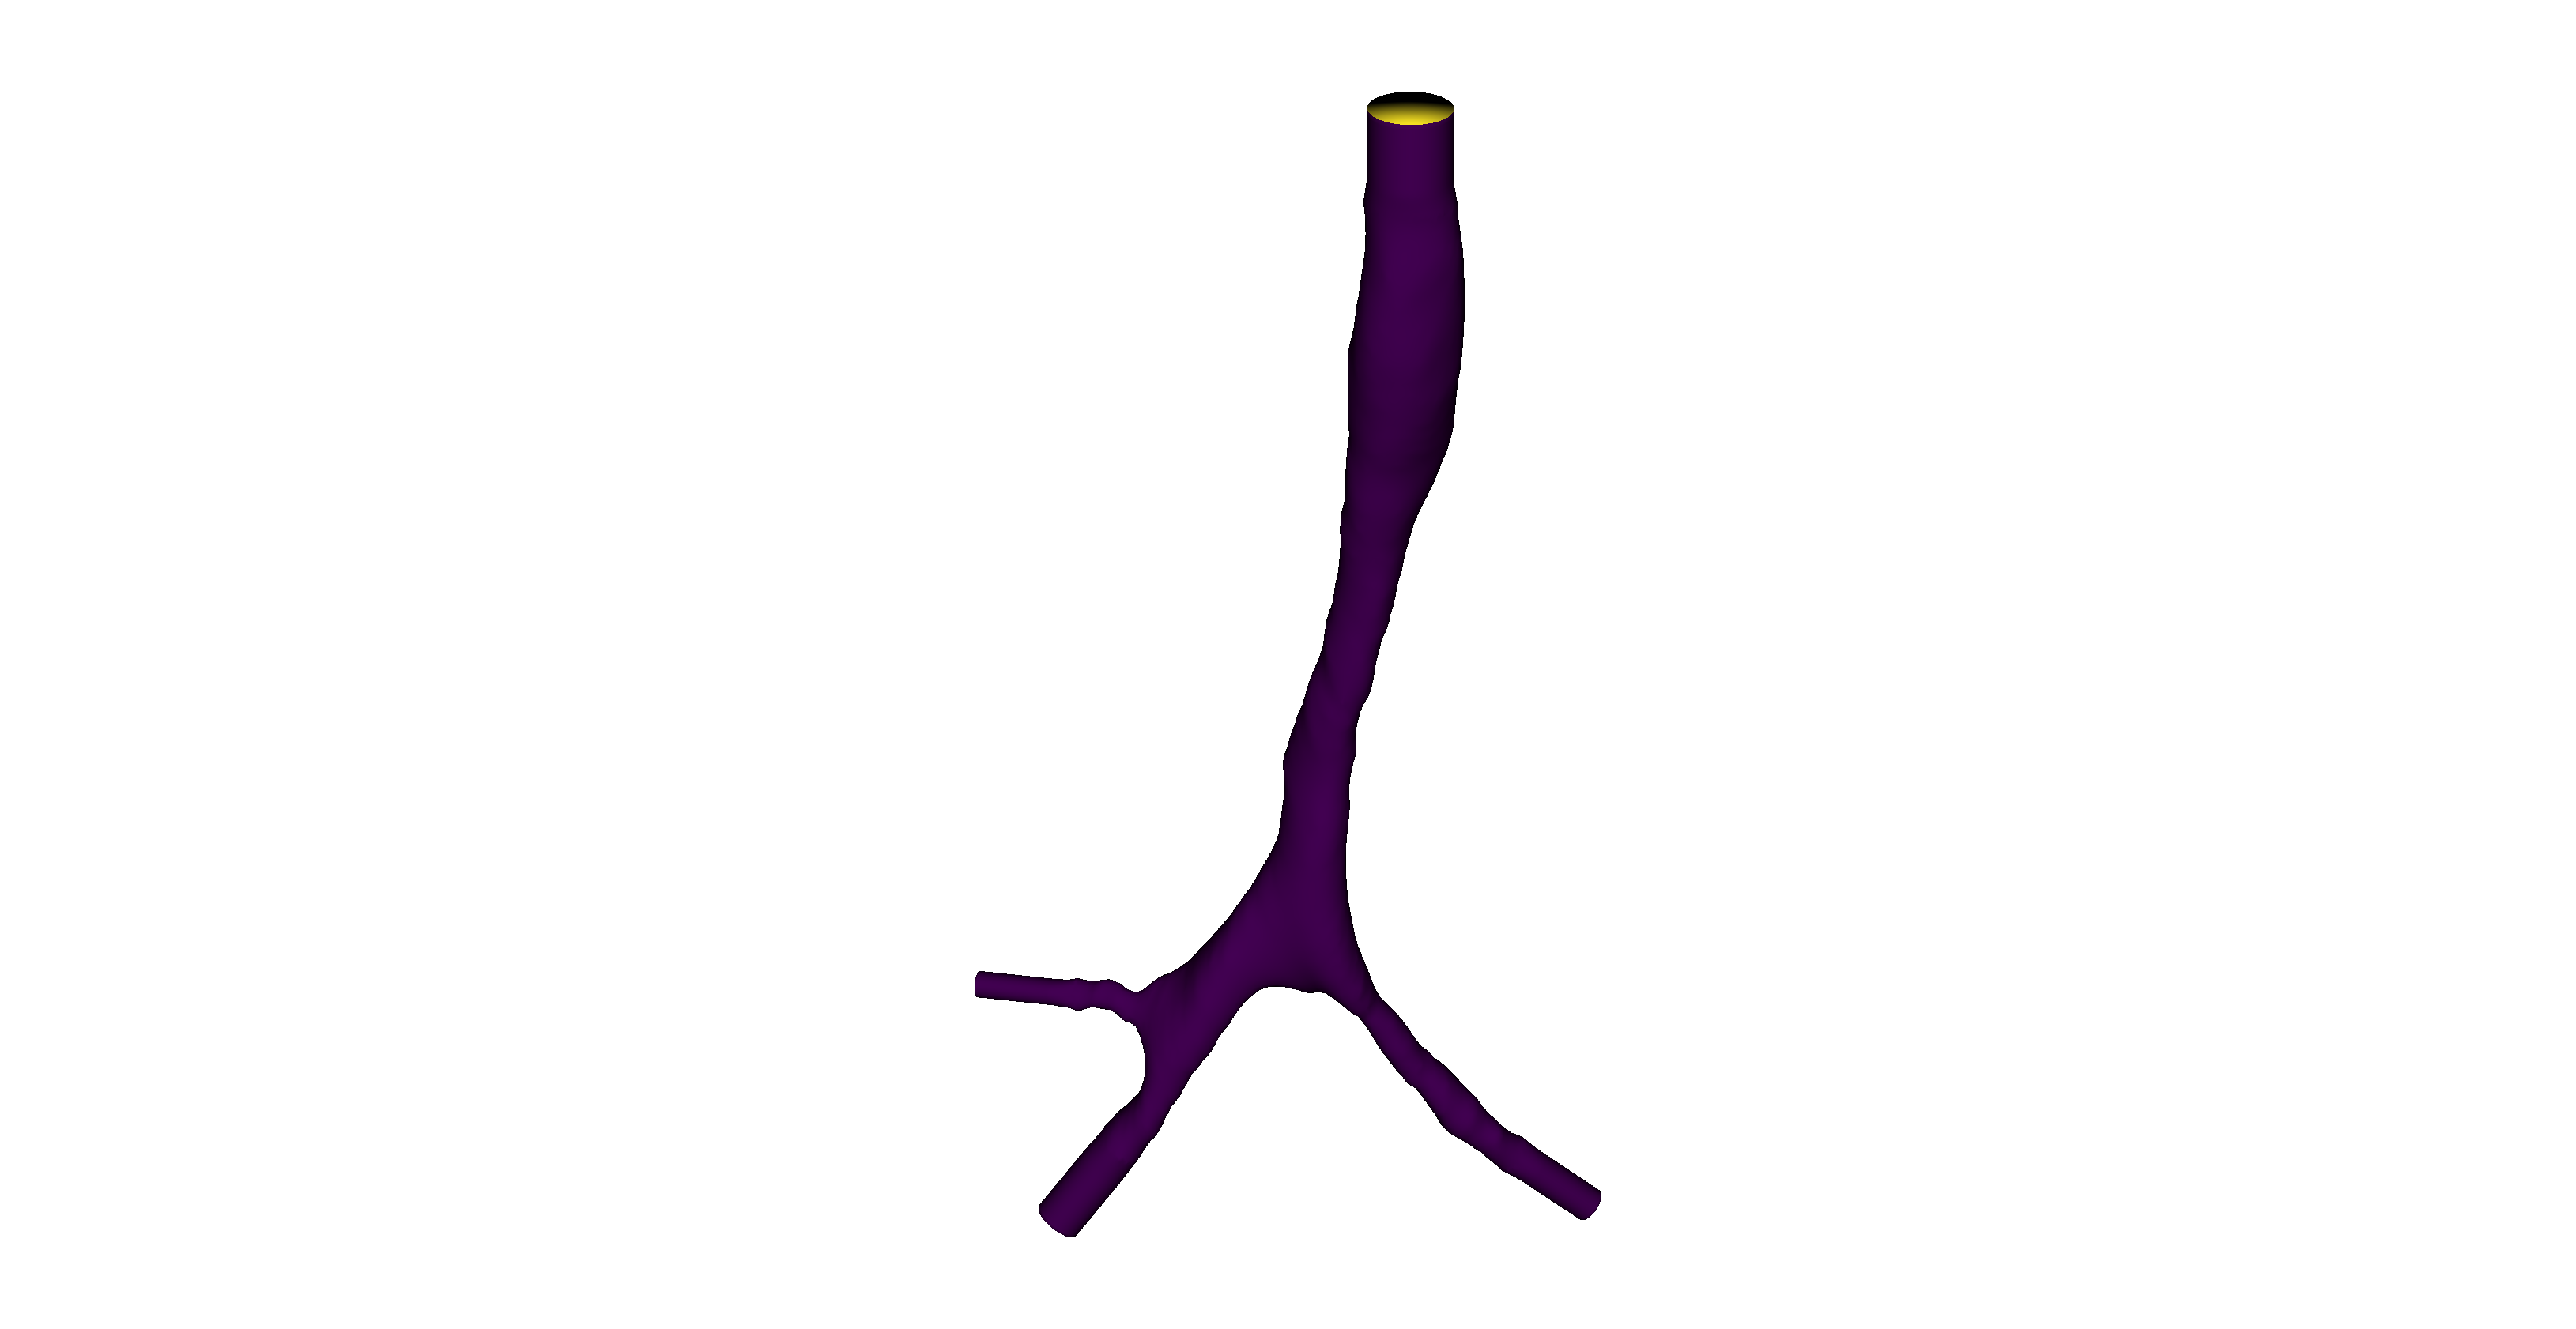
\includegraphics[width=\linewidth]{postop_cfd_surface.png}
    \caption{Postoperative clipped, extended, and capped surface.}
  \end{subfigure}
  \caption{Case-specific airway preparation in anatomical frontal view. The top
  row shows the live Slicer segmentations; the bottom row shows the final CFD
  surfaces with centerline-directed flow extensions and planar caps.}
  \label{fig:segmentation}
\end{figure}

\subsection{Anatomical measurements and degree of constriction}
\label{sec:anatomical_measurements}

The preoperative constriction is bounded by proximal and distal landmarks on the
tracheal centerline. Its length is measured along that centerline. Cross-sections
normal to the local centerline are sampled through the narrowed region to locate
the minimum lumen area. Because the lumen need not be circular, an equivalent
circular diameter is calculated from section area $A$ as

\begin{equation}
  D_{\mathrm{eq}} = 2\sqrt{\frac{A}{\pi}}.
\end{equation}

The postoperative area and equivalent diameter are measured using the same
procedure at 76.53\% of the inlet-to-carina centerline length. The carina is
defined from the airway-network bifurcation nearest the airway seed. The primary
area-based degree of constriction is

\begin{equation}
  C_A = \left(1-\frac{A_{\mathrm{pre,min}}}
  {A_{\mathrm{post,matched}}}\right)\times 100\%.
  \label{eq:area_constriction}
\end{equation}

The measured area constriction is 64.9\%. For transparency, the corresponding
minimum-Feret-diameter reduction is 65.2\% and is reported as

\begin{equation}
  C_D = \left(1-\frac{D_{\mathrm{pre,min}}}
  {D_{\mathrm{post,matched}}}\right)\times 100\%.
\end{equation}

\begin{table}[htbp]
  \centering
  \caption{Anatomical measurements obtained from centerline-normal lumen
  sections in 3D Slicer.}
  \label{tab:anatomical_measurements}
  \begin{tabular}{@{}lll@{}}
    \toprule
    Quantity & Symbol & Value \\
    \midrule
    Preoperative constriction length & $L_{\mathrm{pre}}$ & 12.157 \si{\milli\metre} \\
    Preoperative minimum area & $A_{\mathrm{pre,min}}$ & 1.813 \si{\milli\metre\squared} \\
    Preoperative minimum Feret diameter & $D_{\mathrm{pre,Feret}}$ & 0.798 \si{\milli\metre} \\
    Preoperative equivalent diameter & $D_{\mathrm{pre,eq}}$ & 1.519 \si{\milli\metre} \\
    Postoperative matched area & $A_{\mathrm{post,matched}}$ & 5.169 \si{\milli\metre\squared} \\
    Postoperative minimum Feret diameter & $D_{\mathrm{post,Feret}}$ & 2.292 \si{\milli\metre} \\
    Postoperative equivalent diameter & $D_{\mathrm{post,eq}}$ & 2.565 \si{\milli\metre} \\
    Area constriction & $C_A$ & 64.9\% \\
    Minimum Feret diameter reduction & $C_{D,\mathrm{Feret}}$ & 65.2\% \\
    \bottomrule
  \end{tabular}
\end{table}

The measured dimensions are consistent with the scale reported in paediatric
tracheal-surgery literature. Arcieri et al. described 25 children with congenital
tracheal stenosis and reported a mean internal diameter of
\SI{1.5}{\milli\metre}; the cohort had a median operative age of seven months and
median weight of \SI{5.2}{\kilogram} \cite{arcieri2018}. This closely matches the
\SI{1.519}{\milli\metre} preoperative equivalent diameter obtained here. The
smaller minimum Feret diameter of \SI{0.798}{\milli\metre} is not contradictory:
it characterises the narrowest caliper dimension of a non-circular lumen, whereas
the equivalent diameter is derived from total cross-sectional area. The
literature comparison supports dimensional plausibility but is not an independent
validation of the patient-specific segmentation or landmark placement.

\begin{figure}[htbp]
  \centering
  \begin{subfigure}[t]{0.48\textwidth}
    \centering
    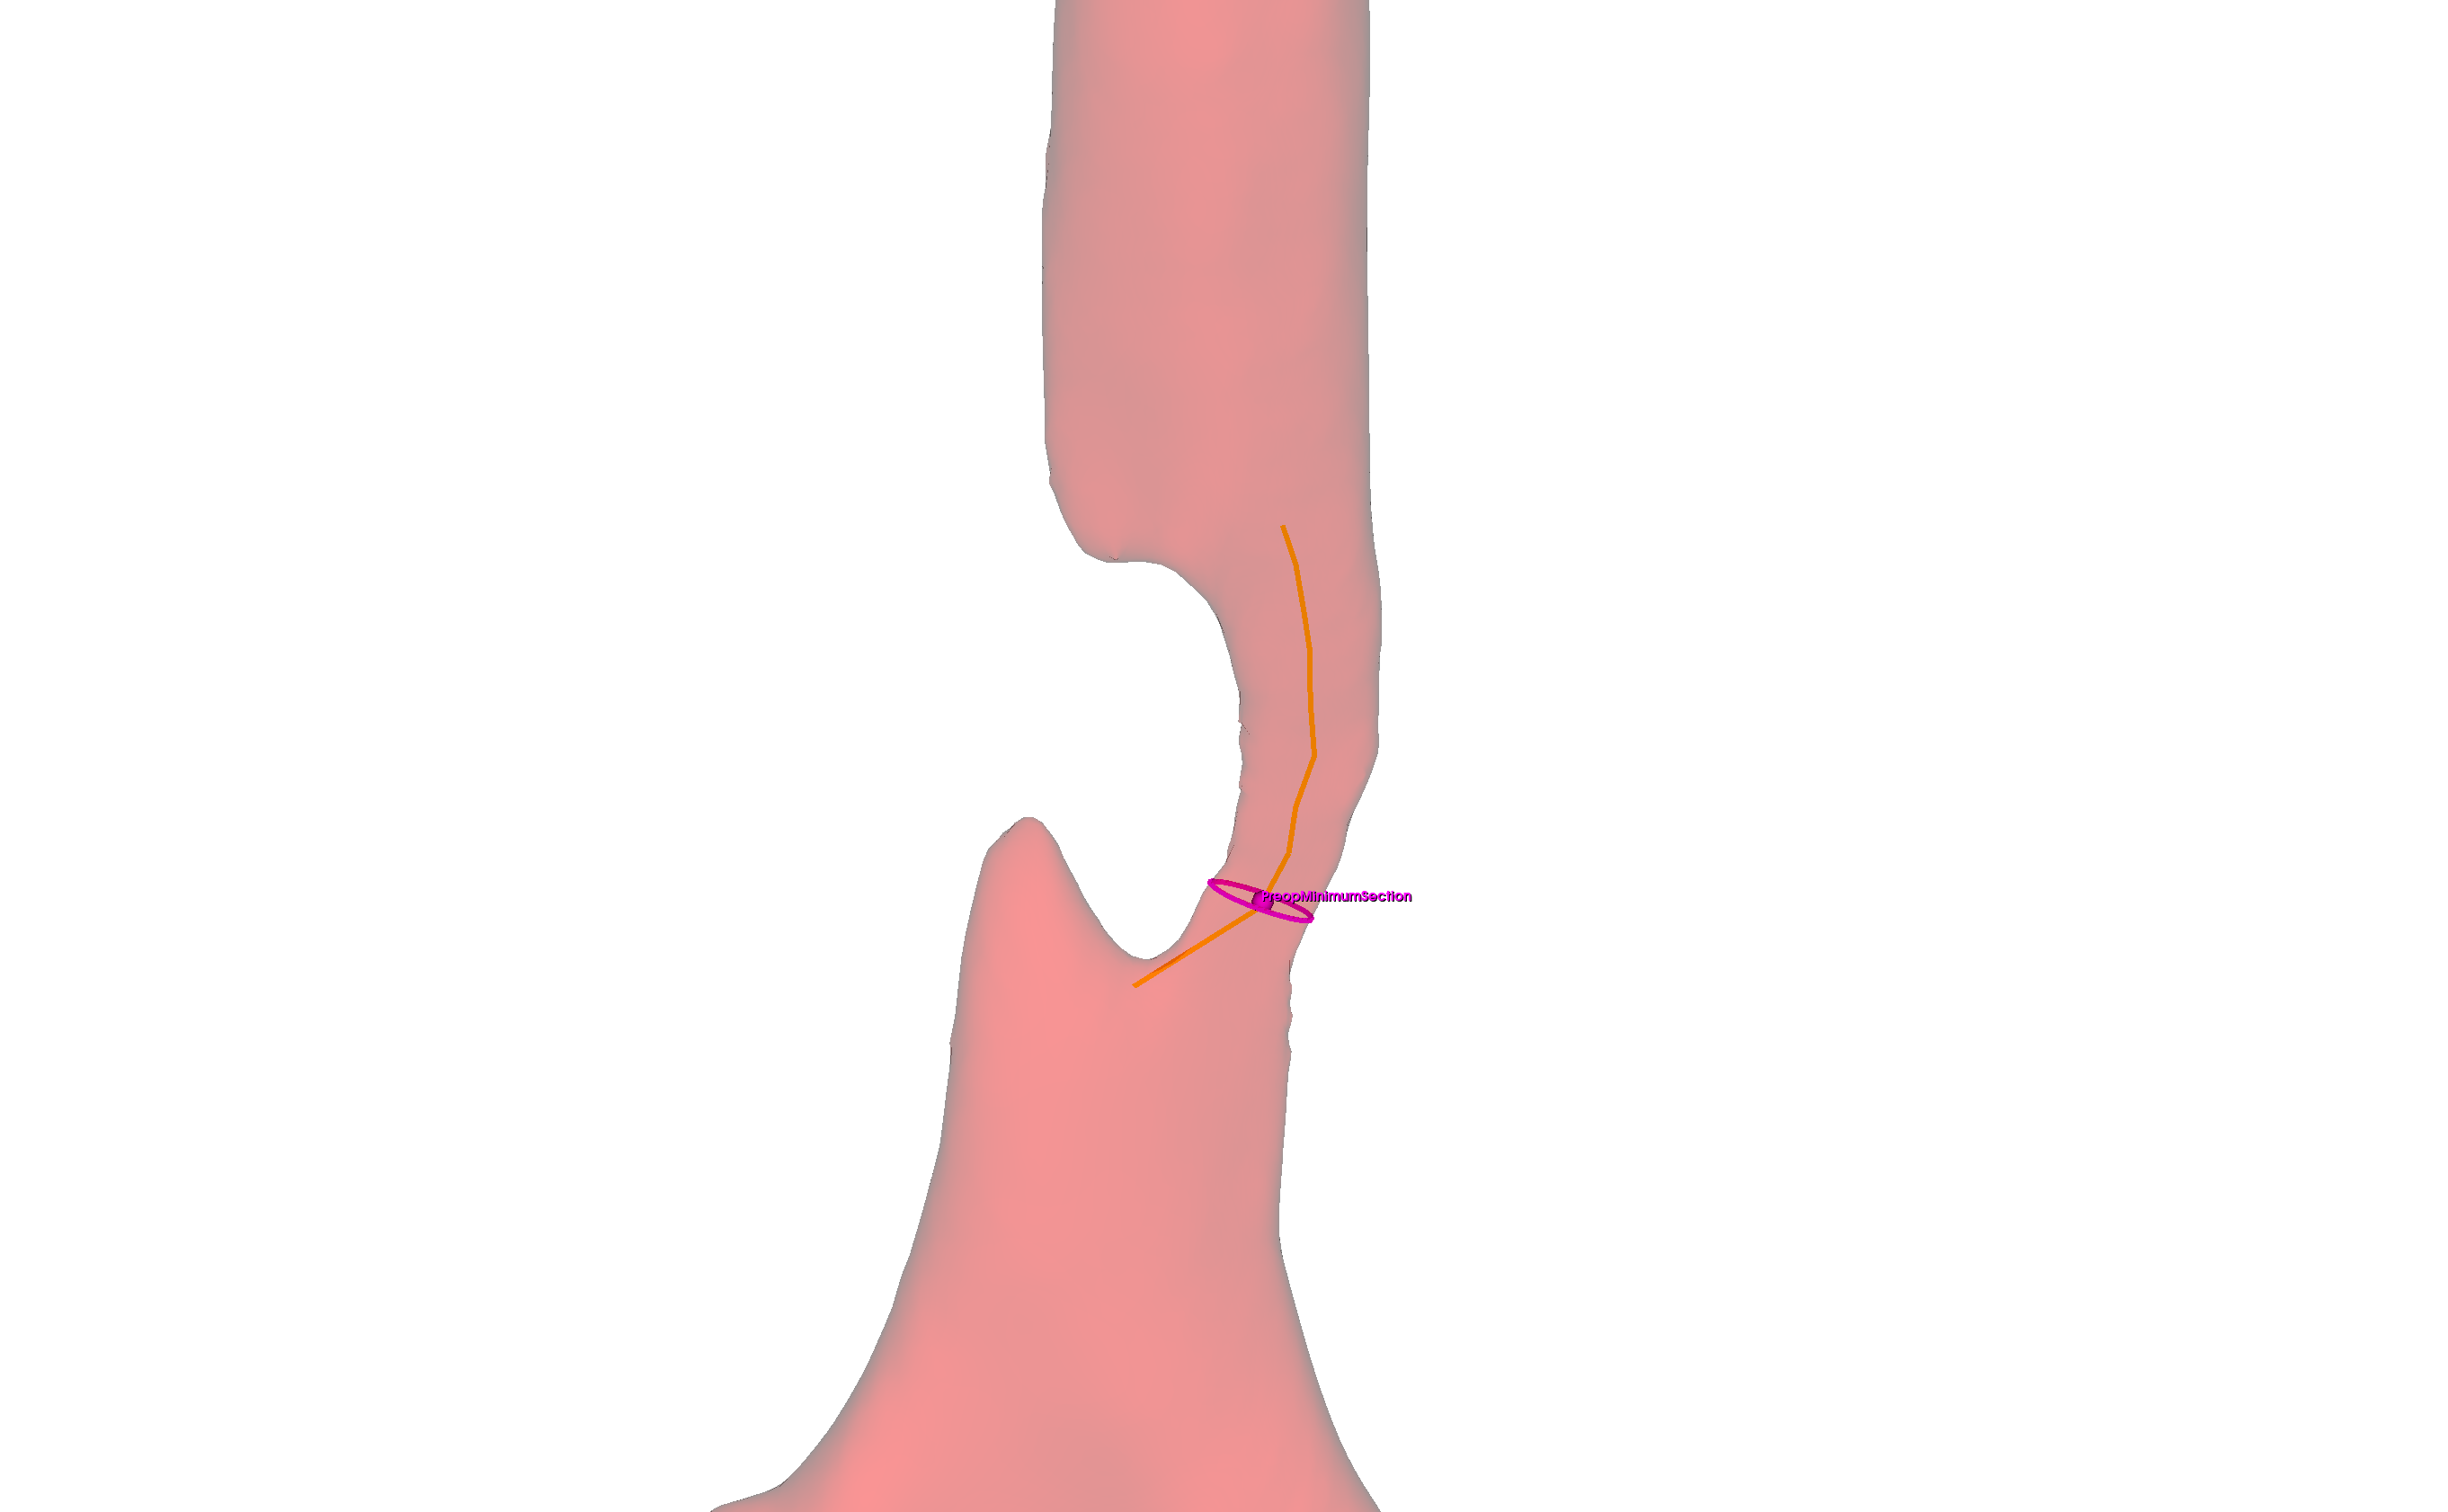
\includegraphics[width=\linewidth]{preop_stenosis_measurement.png}
    \caption{Preoperative stenosis path and minimum section.}
  \end{subfigure}\hfill
  \begin{subfigure}[t]{0.48\textwidth}
    \centering
    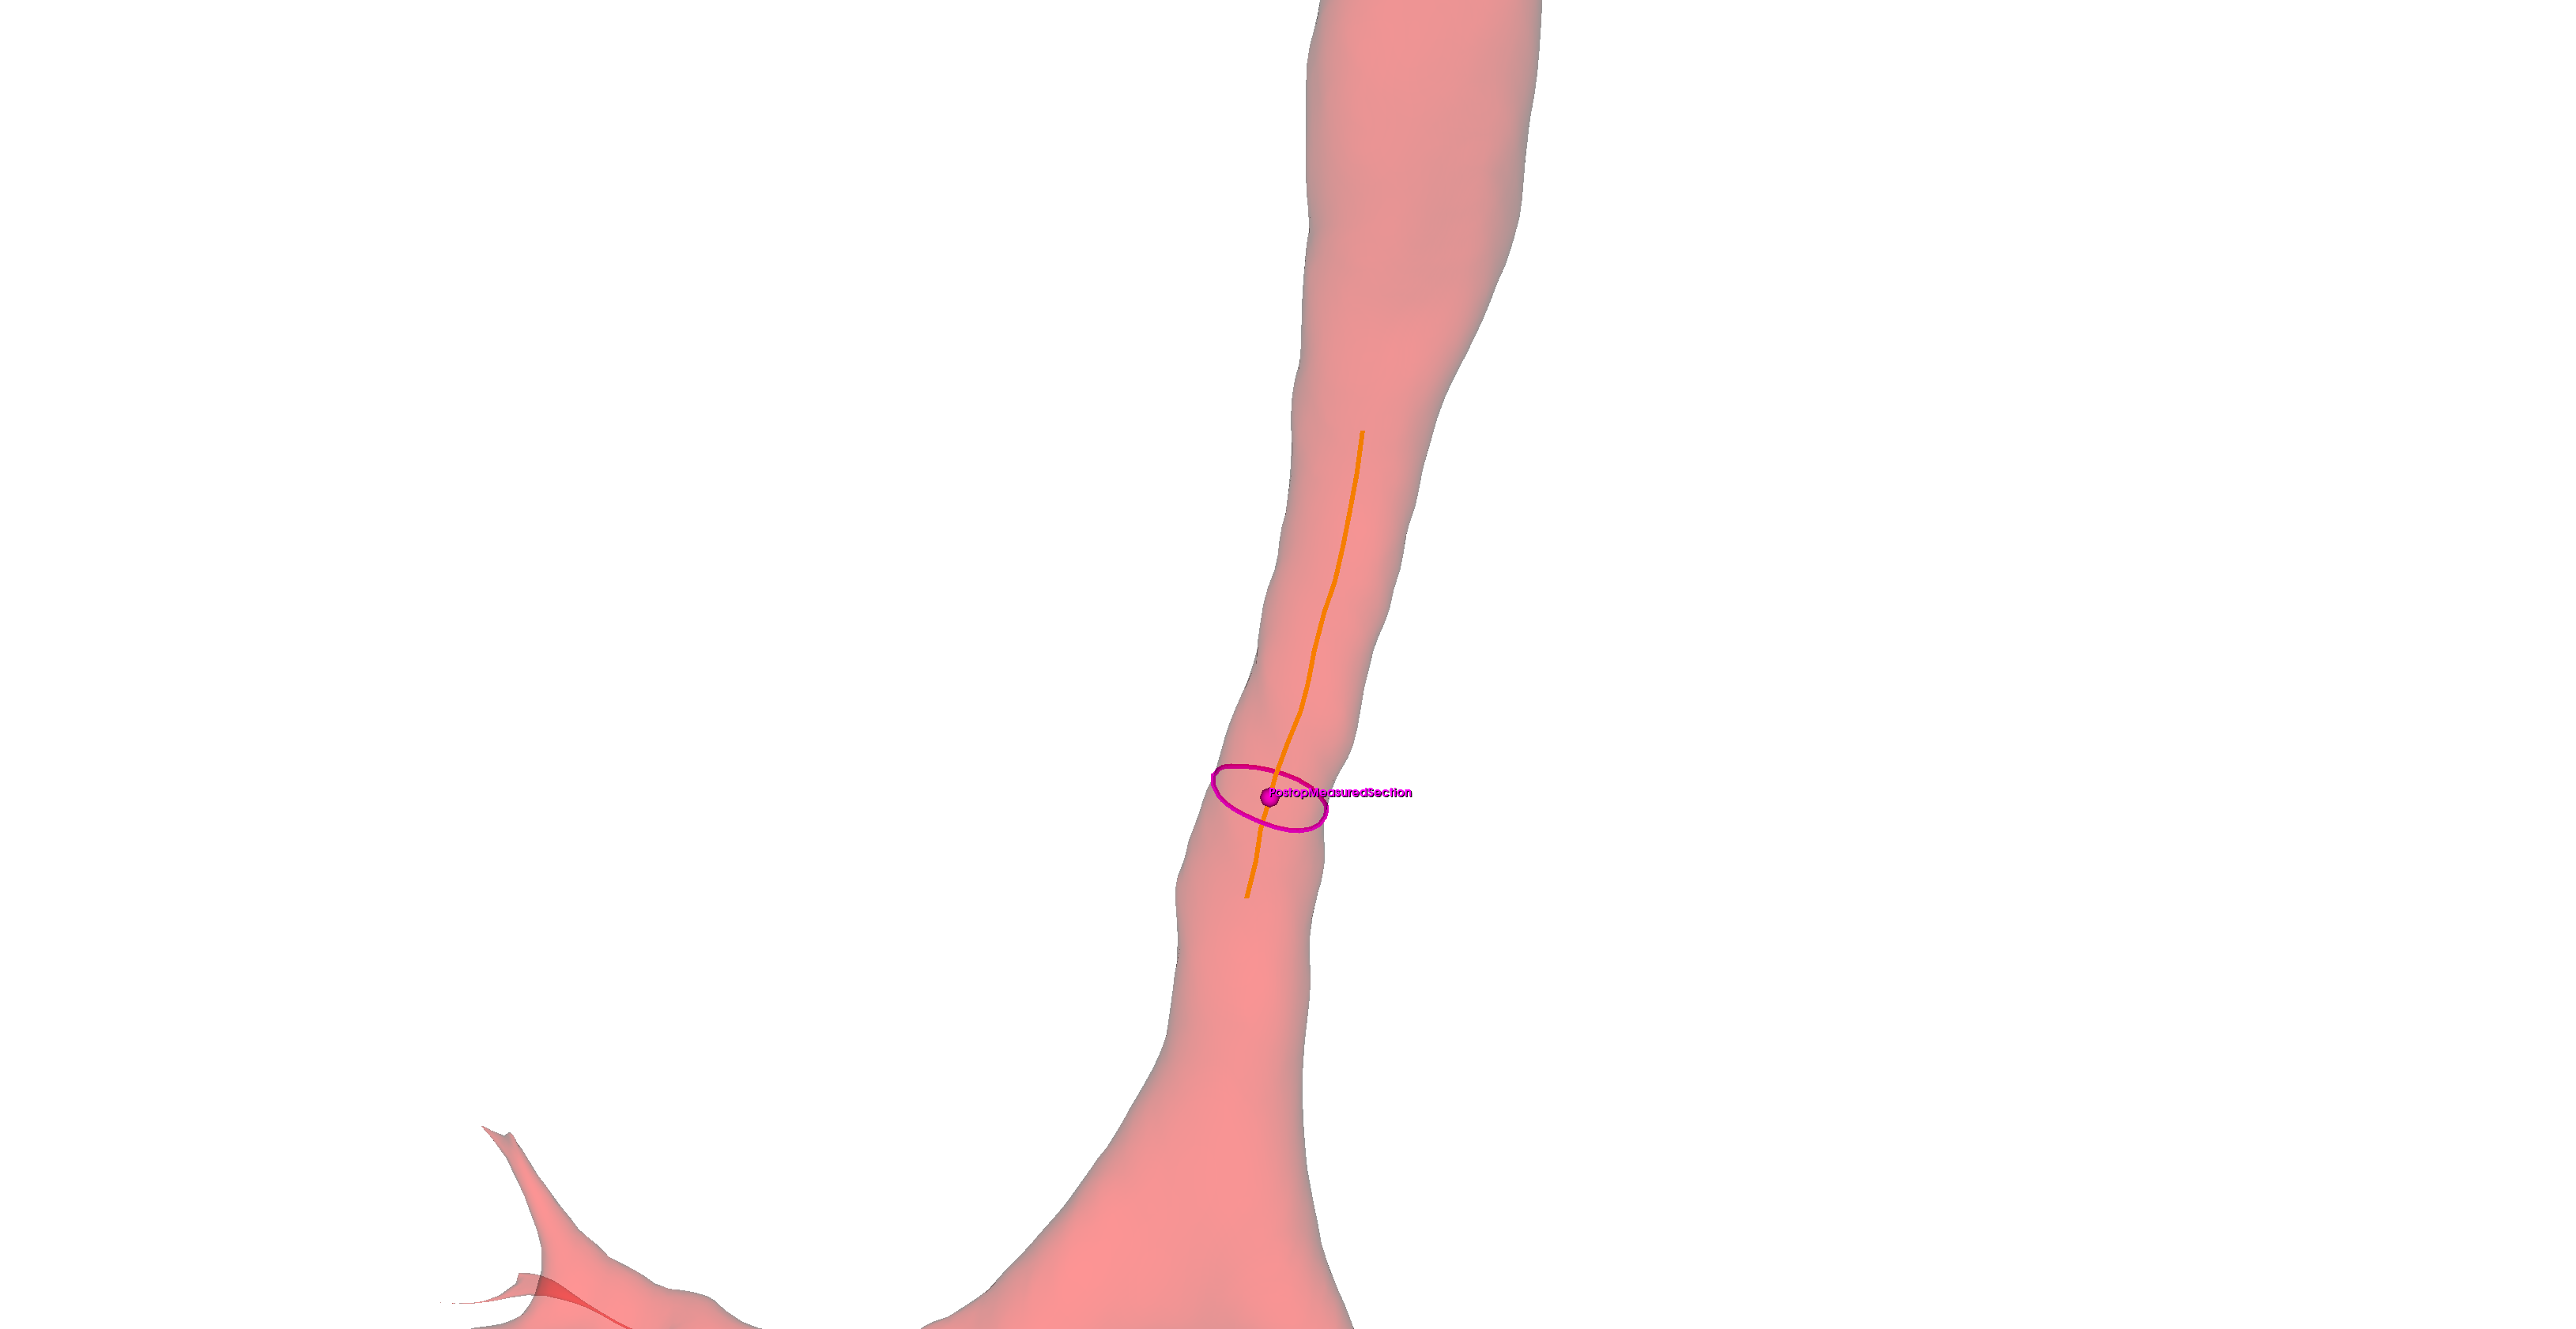
\includegraphics[width=\linewidth]{postop_matched_section.png}
    \caption{Mapped postoperative comparison section.}
  \end{subfigure}
  \caption{Centerline-based anatomical correspondence. Orange curves show the
  measured tracheal interval and magenta contours identify the preoperative
  minimum and corresponding postoperative lumen sections. The postoperative
  location is mapped using 76.53\% of inlet-to-carina centerline distance.}
  \label{fig:anatomical_measurements}
\end{figure}

\subsection{Qualitative flow behaviour through the constriction}

For incompressible flow, continuity $Q=AU$ requires velocity to rise as the area
narrows and fall after expansion. Before the stenosis, pressure decreases
gradually because viscous wall shear opposes motion; for laminar circular flow,
$\Delta p=128\mu LQ/(\pi D^4)$. Through the stenosis, acceleration converts
static pressure into kinetic energy according to Bernoulli's principle, while
viscosity and separation add irreversible loss. Downstream, deceleration causes
partial pressure recovery, but pressure remains below the upstream trend because
separation, mixing, and wall friction dissipate mechanical energy.

\begin{figure}[htbp]
  \centering
  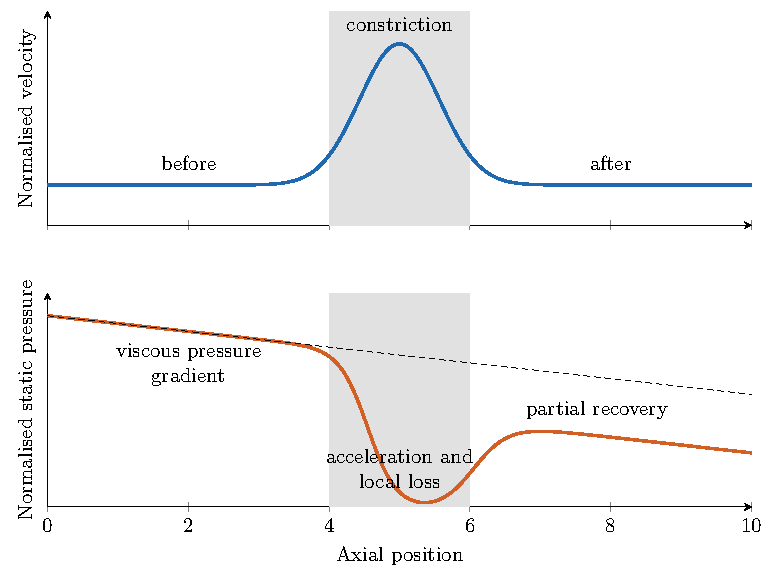
\includegraphics[width=0.88\textwidth]{assignment3_flow_behavior.pdf}
  \caption{Qualitative velocity and static-pressure evolution through a
  constriction. Velocity increases as area decreases; pressure falls sharply
  through the stenosis and recovers only partially downstream. Curves are
  schematic and not CFD results.}
  \label{fig:assignment3_flow_behavior}
\end{figure}

% -----------------------------------------------------------------------------
\section{Volume mesh generation}
\label{sec:mesh}

The triangulated STL surface is imported into Gmsh. Surface classification and
geometry creation produce a closed fluid volume. The physical boundary groups
are:

\begin{itemize}
  \item \texttt{inlet}: tracheal inlet;
  \item \texttt{outlet\_1}: right superior lobar bronchus;
  \item \texttt{outlet\_2}: right inferior lobar bronchus;
  \item \texttt{outlet\_3}: left main bronchus;
  \item \texttt{wall}: remaining airway surface; and
  \item \texttt{fluid}: internal volume.
\end{itemize}

The physical groups are visually verified whenever the STL topology or Gmsh
classification changes. The volume consists of first-order tetrahedra with a
uniform target characteristic length controlled by \texttt{MESH\_SIZE}.

\begin{table}[htbp]
  \centering
  \caption{Replicable mesh settings and quality metrics. All current volume
  elements are first-order tetrahedra. Add the exact Gmsh version and final
  values from each \texttt{checkMesh} log.}
  \label{tab:meshes}
  \resizebox{\textwidth}{!}{%
  \begin{tabular}{@{}lrrrrrr@{}}
    \toprule
    Mesh & Target size (mm) & Points & Cells & Element type & Max. aspect ratio & Max. non-orthogonality \\
    \midrule
    HXT baseline & 0.25 & 39,977  & 180,163   & Tetrahedron & 114.14 & 88.63$^\circ$ \\
    HXT fine 1   & 0.20 & 71,198  & 339,886   & Tetrahedron & 11.73  & 80.29$^\circ$ \\
    HXT fine 2   & 0.15 & 151,599 & 776,568   & Tetrahedron & 12.63  & 69.82$^\circ$ \\
    HXT densest  & 0.12 & 281,330 & 1,493,440 & Tetrahedron & 88.00  & 82.34$^\circ$ \\
    \bottomrule
  \end{tabular}%
  }
\end{table}

\subsection{Near-wall resolution}

Boundary-layer prism elements are commonly used near no-slip walls because they
resolve steep wall-normal velocity gradients efficiently and with better cell
alignment than isotropic tetrahedra. The current Gmsh workflow uses only
first-order tetrahedra and does not include dedicated inflation layers. This
must not be presented as a hybrid boundary-layer mesh. Its consequences are
considered when interpreting wall-adjacent quantities, and adding prism layers
is identified as a model improvement.

The Gmsh mesh uses millimetres because it inherits the Slicer coordinate scale.
After \texttt{gmshToFoam}, all coordinates are multiplied by $10^{-3}$ to obtain
SI units.

\begin{figure}[htbp]
  \centering
  \begin{subfigure}[t]{0.48\textwidth}
    \centering
    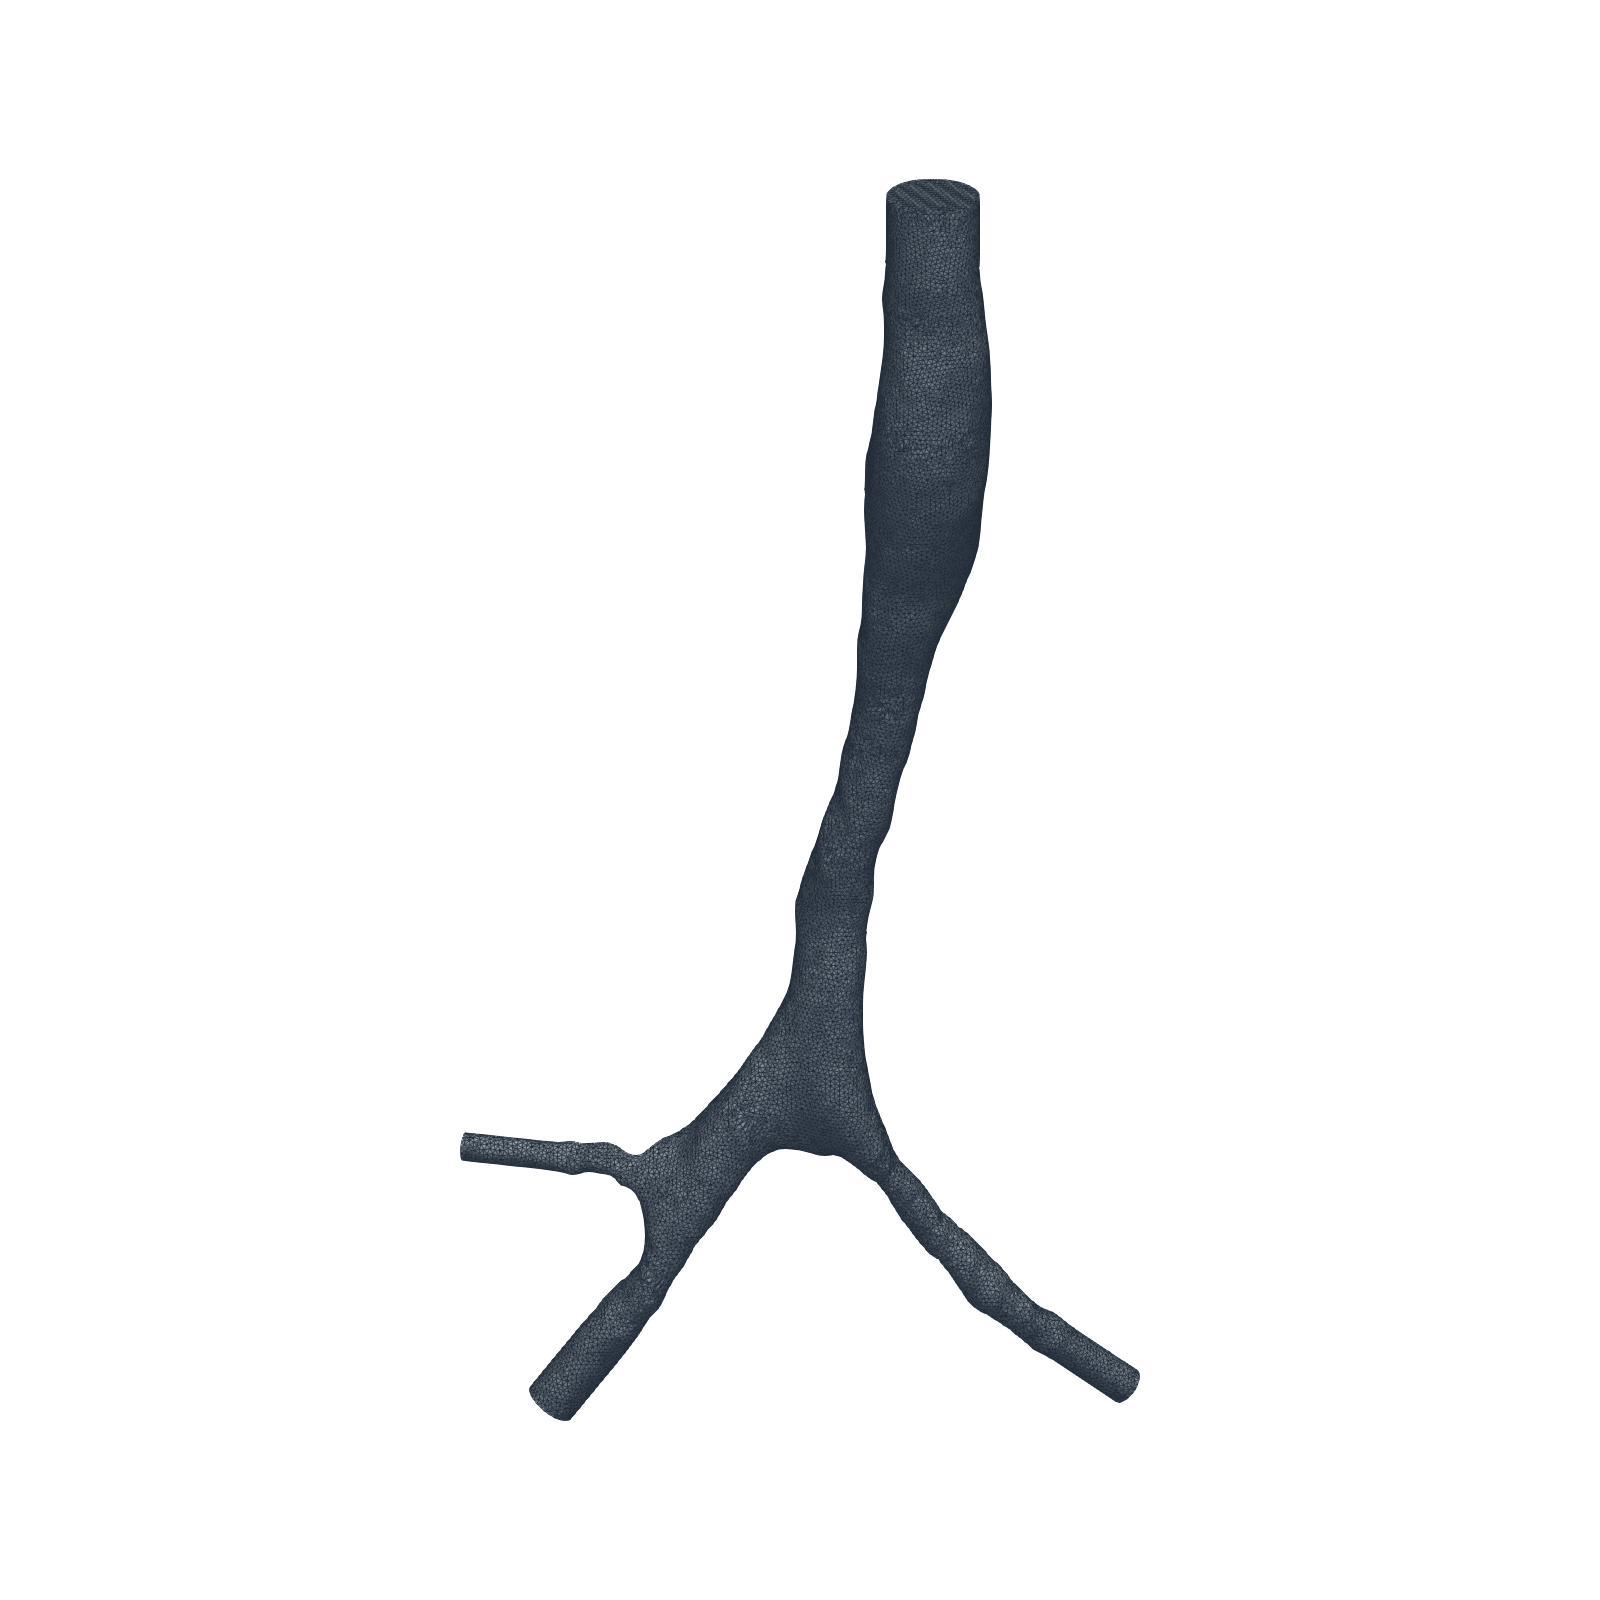
\includegraphics[width=\linewidth]{assignment5_mesh_025_full.png}
    \caption{0.25 mm HXT baseline; 180,163 volume cells.}
  \end{subfigure}\hfill
  \begin{subfigure}[t]{0.48\textwidth}
    \centering
    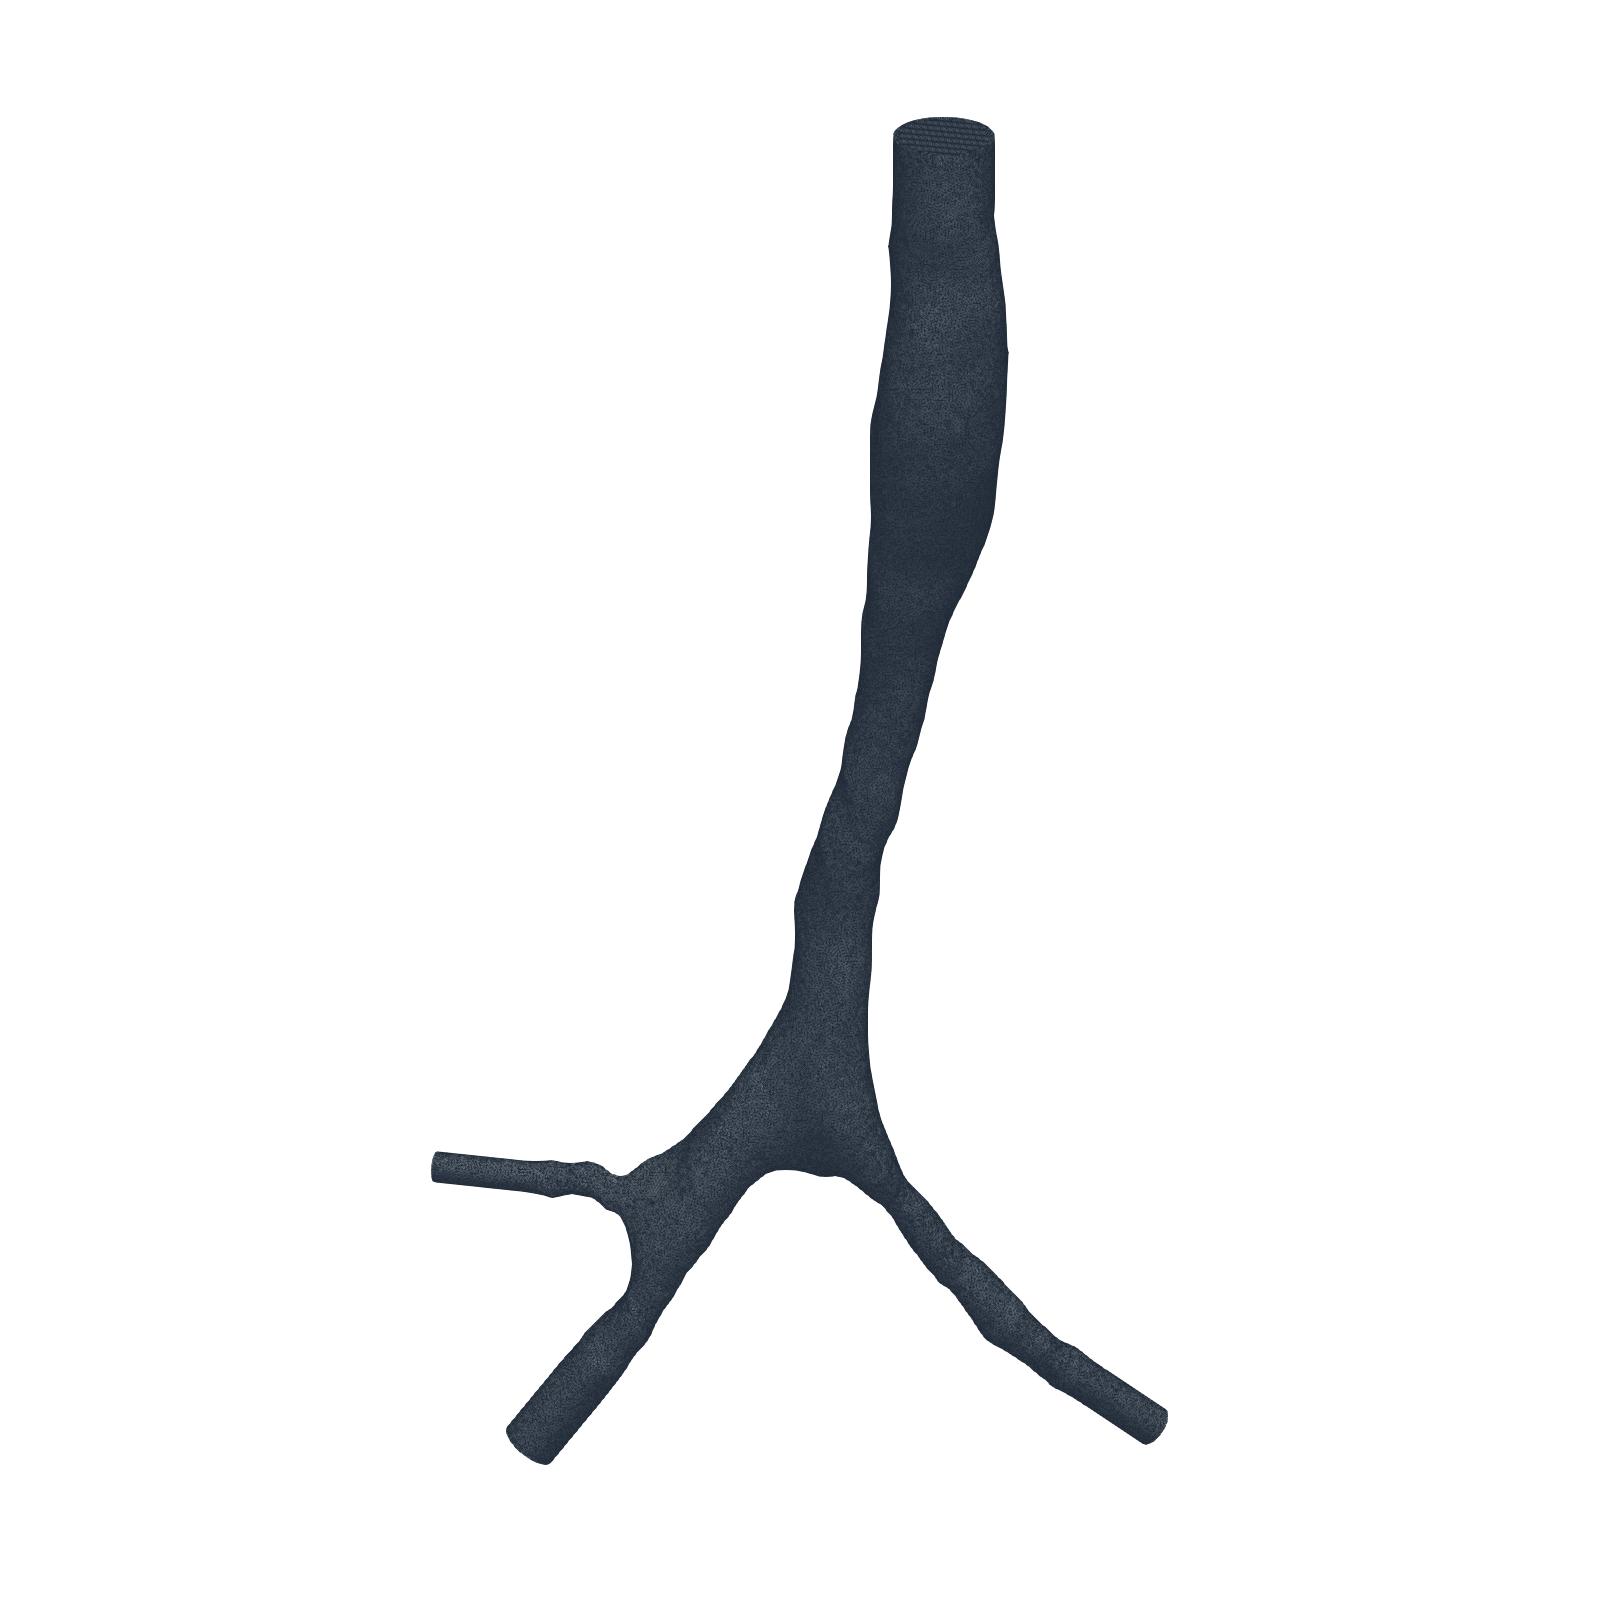
\includegraphics[width=\linewidth]{assignment5_mesh_015_full.png}
    \caption{Selected 0.15 mm HXT mesh; 776,568 volume cells.}
  \end{subfigure}

  \vspace{0.5em}
  \begin{subfigure}[t]{0.48\textwidth}
    \centering
    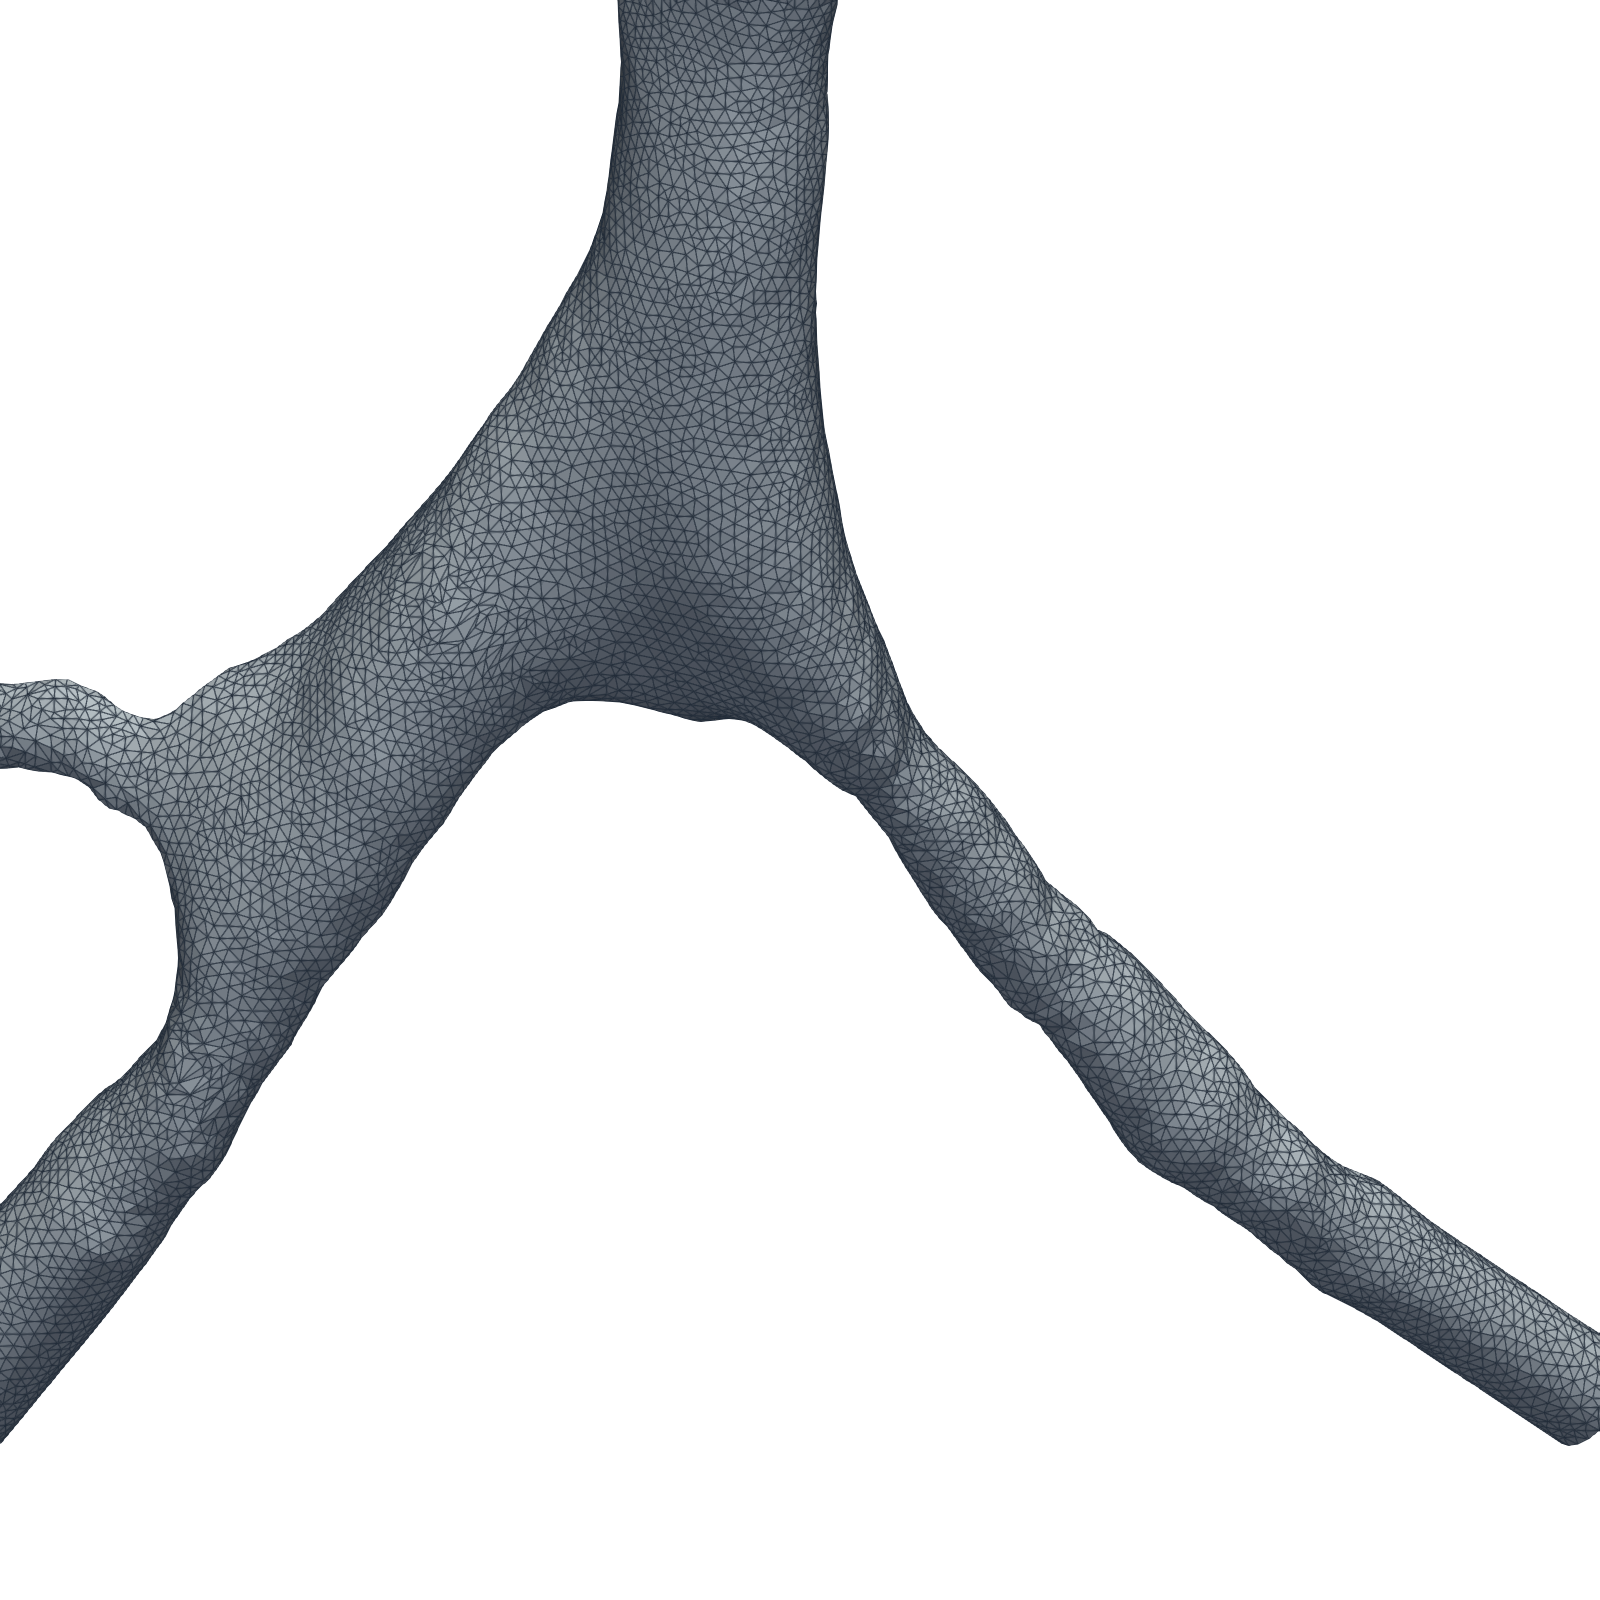
\includegraphics[width=\linewidth]{assignment5_mesh_025_closeup.png}
    \caption{Baseline surface triangulation at the carina.}
  \end{subfigure}\hfill
  \begin{subfigure}[t]{0.48\textwidth}
    \centering
    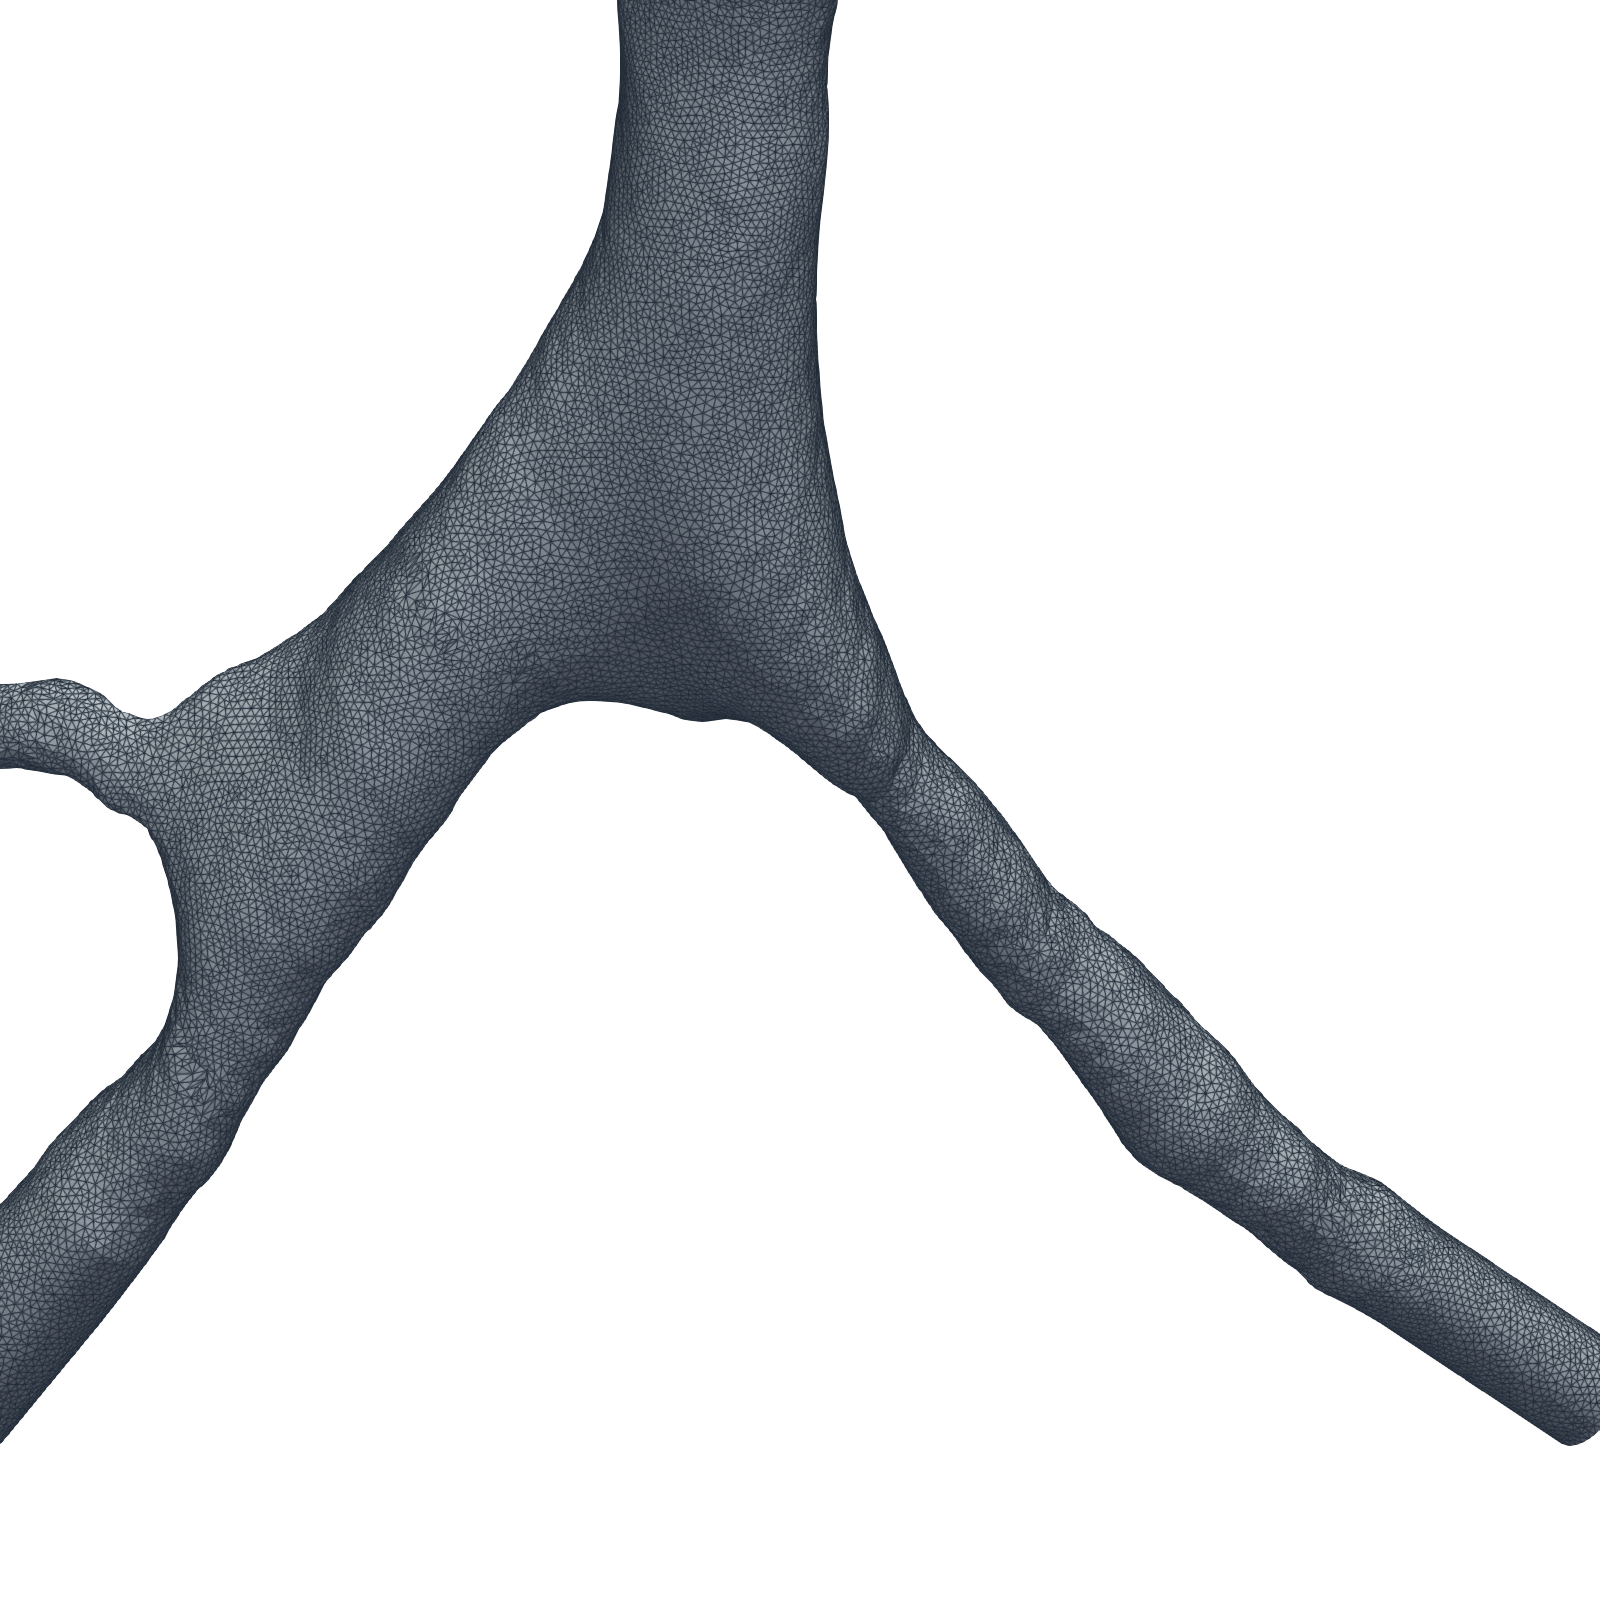
\includegraphics[width=\linewidth]{assignment5_mesh_015_closeup.png}
    \caption{Selected-mesh surface triangulation at the carina.}
  \end{subfigure}
  \caption{Postoperative HXT mesh refinement in matched anatomical frontal
  views. The complete baseline and selected meshes are shown above, with
  identically framed carina close-ups below. Both levels use the same geometry,
  physical surface groups, and HXT algorithm; only target characteristic length
  differs. Surface-edge density illustrates refinement, while quantitative
  volume-mesh sensitivity is assessed separately in
  Section~\ref{sec:mesh_sensitivity}.}
  \label{fig:meshes}
\end{figure}

% -----------------------------------------------------------------------------
\section{Mathematical model}
\label{sec:model}

\subsection{Governing equations}

Air is modelled as an incompressible Newtonian fluid. For steady flow, mass and
momentum conservation are:

\begin{align}
  \nabla \cdot \mathbf{u} &= 0, \\
  \rho (\mathbf{u}\cdot\nabla)\mathbf{u}
    &= -\nabla p + \mu \nabla^2\mathbf{u},
\end{align}

where $\mathbf{u}$ is velocity, $p$ is pressure, $\rho$ is density, and $\mu$
is dynamic viscosity. OpenFOAM uses kinematic pressure and the kinematic
viscosity $\nu=\mu/\rho$. The configured value is
$\nu=\SI{1.5e-5}{\metre\squared\per\second}$.

The current case uses the laminar model and the steady-state
\texttt{simpleFoam} solver. The appropriateness of the laminar assumption should
be assessed using a Reynolds number based on representative velocity $U$ and
diameter $D$:

\begin{equation}
  \mathrm{Re} = \frac{UD}{\nu}.
\end{equation}

[Calculate Reynolds numbers at the inlet and stenosis and discuss whether a
laminar, transitional, or turbulent model is justified.]

\subsection{Boundary conditions}

A prescribed volumetric flow rate is applied at the tracheal inlet:

\begin{equation}
  Q_{\mathrm{in}} = \SI{3.3333e-5}{\metre\cubed\per\second}.
\end{equation}

This corresponds to approximately \SI{2}{\litre\per\minute}, representative
of the stated minute volume for a 10-month-old infant. A no-slip condition is
applied at the airway wall. The three distal outlets use the same zero gauge
pressure with pressure-compatible velocity conditions. No outlet flow fraction
is prescribed; consequently, the flow division is an output of the CFD solution.
For a common downstream pressure, each pathway behaves approximately as

\begin{equation}
  Q_i \sim \frac{\Delta P}{R_i},
\end{equation}

where differences in effective resistance $R_i$ arise from features such as
branch diameter, length, branching angle, curvature, and flow separation.
Table~\ref{tab:bc} summarises the implementation.

\begin{table}[htbp]
  \centering
  \caption{OpenFOAM boundary conditions.}
  \label{tab:bc}
  \begin{tabular}{@{}lll@{}}
    \toprule
    Patch & Velocity $\mathbf{u}$ & Pressure $p$ \\
    \midrule
    \texttt{inlet} & \texttt{flowRateInletVelocity} & \texttt{zeroGradient} \\
    \texttt{outlet\_1--3} & \texttt{pressureInletOutletVelocity} & \texttt{fixedValue 0} \\
    \texttt{wall} & \texttt{noSlip} & \texttt{zeroGradient} \\
    \bottomrule
  \end{tabular}
\end{table}

% -----------------------------------------------------------------------------
\section{Numerical method}
\label{sec:numerics}

The teaching staff approved the use of 3D Slicer and SlicerVMTK for geometry
preparation, Gmsh for meshing, OpenFOAM for CFD, and independent local/remote
compute infrastructure. This changes the software implementation but not the
required physical analyses or validation.

\begin{table}[htbp]
  \centering
  \caption{Software and provenance information. Replace placeholders with the
  immutable versions used for the final simulations.}
  \label{tab:software}
  \begin{tabular}{@{}lll@{}}
    \toprule
    Stage & Software & Version or identifier \\
    \midrule
    Segmentation & 3D Slicer + SlicerVMTK & 5.12.2; extension [insert] \\
    Surface/volume meshing & Gmsh & [insert] \\
    CFD & OpenFOAM Docker image & 2512; image ID [insert] \\
    Post-processing & ParaView & [insert] \\
    Source state & Git & commit [insert] \\
    \bottomrule
  \end{tabular}
\end{table}

\subsection{Steady solver}

The finite-volume discretisation is implemented in OpenFOAM 2512. Pressure is
solved using GAMG and velocity using a symmetric Gauss--Seidel smoothed solver.
The SIMPLE algorithm uses two non-orthogonal correctors. The configured residual
controls are $10^{-5}$ for pressure and $10^{-6}$ for velocity.

The parallel mesh is decomposed using the Scotch method. Simulations are run in
the \texttt{opencfd/openfoam-default:latest} Docker image. The exact image ID
and Git commit are recorded in Table~\ref{tab:software}.

\subsection{Transient solver and breathing waveform}
\label{sec:transient_method}

The selected \num{0.15}~mm HXT mesh is reused for the postoperative transient
simulation. The incompressible, Newtonian equations are solved with
\texttt{pimpleFoam}. A symmetric sinusoidal volumetric-flow boundary condition is
prescribed at the tracheal inlet,
\begin{equation}
  Q(t)=Q_{\max}\sin\left(\frac{2\pi t}{T}\right),
\end{equation}
where $T=\SI{2.0}{\second}$ and
$Q_{\max}=\SI{1.0472e-4}{\metre\cubed\per\second}$
(\SI{6.283}{\litre\per\minute}). The positive half-cycle represents inspiration
and the negative half-cycle expiration. Integrating either half-cycle gives a
tidal volume of \SI{66.7}{\milli\litre}, consistent with the assumed
\SI{2}{\litre\per\minute} minute ventilation at 30 breaths per minute.

The inlet uses \texttt{flowRateInletVelocity}. All three outlets have zero fixed
kinematic pressure and \texttt{pressureInletOutletVelocity}, which permits flow
reversal during expiration. The rigid airway wall remains no-slip. Time is
discretised with the second-order backward scheme. Three PIMPLE outer correctors,
two pressure correctors, and one non-orthogonal corrector are used. An initial
time step of \SI{1e-5}{\second} is adjusted subject to $\mathrm{Co}_{\max}=2$
and a maximum step of \SI{5e-5}{\second}; fields are written every
\SI{0.02}{\second}. The original $\mathrm{Co}_{\max}=1$ timing test was rejected
because a small subset of cells forced the step below \SI{1e-5}{\second} while
the mean Courant number remained below 0.08. A \SI{0.05}{\second} timing run and
a subsequent pilot through \SI{0.55}{\second} precede the complete cycle. Pilot
results determine whether these controls are adequate;
periodicity cannot be claimed from a single cycle and will be assessed by
comparing corresponding quantities in consecutive cycles if an additional cycle
is required.

At the estimated peak mean velocity of approximately
\SI{20.3}{\metre\per\second} in the matched section, the Mach number is about
0.06, supporting the incompressibility approximation. The corresponding Reynolds
number is approximately 3500, so transitional effects remain a model limitation.
A shorter, more realistic mechanically ventilated inspiratory phase would require
a larger peak flow for the same tidal volume and could approach the commonly used
$\mathrm{Ma}=0.1$ compressibility threshold.

\begin{figure}[htbp]
  \centering
  \resizebox{0.88\textwidth}{!}{% GNUPLOT: LaTeX picture with Postscript
\begingroup
  \makeatletter
  \providecommand\color[2][]{%
    \GenericError{(gnuplot) \space\space\space\@spaces}{%
      Package color not loaded in conjunction with
      terminal option `colourtext'%
    }{See the gnuplot documentation for explanation.%
    }{Either use 'blacktext' in gnuplot or load the package
      color.sty in LaTeX.}%
    \renewcommand\color[2][]{}%
  }%
  \providecommand\includegraphics[2][]{%
    \GenericError{(gnuplot) \space\space\space\@spaces}{%
      Package graphicx or graphics not loaded%
    }{See the gnuplot documentation for explanation.%
    }{The gnuplot epslatex terminal needs graphicx.sty or graphics.sty.}%
    \renewcommand\includegraphics[2][]{}%
  }%
  \providecommand\rotatebox[2]{#2}%
  \@ifundefined{ifGPcolor}{%
    \newif\ifGPcolor
    \GPcolortrue
  }{}%
  \@ifundefined{ifGPblacktext}{%
    \newif\ifGPblacktext
    \GPblacktexttrue
  }{}%
  % define a \g@addto@macro without @ in the name:
  \let\gplgaddtomacro\g@addto@macro
  % define empty templates for all commands taking text:
  \gdef\gplbacktext{}%
  \gdef\gplfronttext{}%
  \makeatother
  \ifGPblacktext
    % no textcolor at all
    \def\colorrgb#1{}%
    \def\colorgray#1{}%
  \else
    % gray or color?
    \ifGPcolor
      \def\colorrgb#1{\color[rgb]{#1}}%
      \def\colorgray#1{\color[gray]{#1}}%
      \expandafter\def\csname LTw\endcsname{\color{white}}%
      \expandafter\def\csname LTb\endcsname{\color{black}}%
      \expandafter\def\csname LTa\endcsname{\color{black}}%
      \expandafter\def\csname LT0\endcsname{\color[rgb]{1,0,0}}%
      \expandafter\def\csname LT1\endcsname{\color[rgb]{0,1,0}}%
      \expandafter\def\csname LT2\endcsname{\color[rgb]{0,0,1}}%
      \expandafter\def\csname LT3\endcsname{\color[rgb]{1,0,1}}%
      \expandafter\def\csname LT4\endcsname{\color[rgb]{0,1,1}}%
      \expandafter\def\csname LT5\endcsname{\color[rgb]{1,1,0}}%
      \expandafter\def\csname LT6\endcsname{\color[rgb]{0,0,0}}%
      \expandafter\def\csname LT7\endcsname{\color[rgb]{1,0.3,0}}%
      \expandafter\def\csname LT8\endcsname{\color[rgb]{0.5,0.5,0.5}}%
    \else
      % gray
      \def\colorrgb#1{\color{black}}%
      \def\colorgray#1{\color[gray]{#1}}%
      \expandafter\def\csname LTw\endcsname{\color{white}}%
      \expandafter\def\csname LTb\endcsname{\color{black}}%
      \expandafter\def\csname LTa\endcsname{\color{black}}%
      \expandafter\def\csname LT0\endcsname{\color{black}}%
      \expandafter\def\csname LT1\endcsname{\color{black}}%
      \expandafter\def\csname LT2\endcsname{\color{black}}%
      \expandafter\def\csname LT3\endcsname{\color{black}}%
      \expandafter\def\csname LT4\endcsname{\color{black}}%
      \expandafter\def\csname LT5\endcsname{\color{black}}%
      \expandafter\def\csname LT6\endcsname{\color{black}}%
      \expandafter\def\csname LT7\endcsname{\color{black}}%
      \expandafter\def\csname LT8\endcsname{\color{black}}%
    \fi
  \fi
    \setlength{\unitlength}{0.0500bp}%
    \ifx\gptboxheight\undefined%
      \newlength{\gptboxheight}%
      \newlength{\gptboxwidth}%
      \newsavebox{\gptboxtext}%
    \fi%
    \setlength{\fboxrule}{0.5pt}%
    \setlength{\fboxsep}{1pt}%
    \definecolor{tbcol}{rgb}{1,1,1}%
\begin{picture}(8500.00,4520.00)%
    \gplgaddtomacro\gplbacktext{%
      \csname LTb\endcsname%%
      \put(487,562){\makebox(0,0)[r]{\strut{}$-8$}}%
      \csname LTb\endcsname%%
      \put(487,989){\makebox(0,0)[r]{\strut{}$-6$}}%
      \csname LTb\endcsname%%
      \put(487,1415){\makebox(0,0)[r]{\strut{}$-4$}}%
      \csname LTb\endcsname%%
      \put(487,1841){\makebox(0,0)[r]{\strut{}$-2$}}%
      \csname LTb\endcsname%%
      \put(487,2267){\makebox(0,0)[r]{\strut{}$0$}}%
      \csname LTb\endcsname%%
      \put(487,2693){\makebox(0,0)[r]{\strut{}$2$}}%
      \csname LTb\endcsname%%
      \put(487,3119){\makebox(0,0)[r]{\strut{}$4$}}%
      \csname LTb\endcsname%%
      \put(487,3546){\makebox(0,0)[r]{\strut{}$6$}}%
      \csname LTb\endcsname%%
      \put(487,3972){\makebox(0,0)[r]{\strut{}$8$}}%
      \csname LTb\endcsname%%
      \put(576,386){\makebox(0,0){\strut{}$0$}}%
      \csname LTb\endcsname%%
      \put(2485,386){\makebox(0,0){\strut{}$0.5$}}%
      \csname LTb\endcsname%%
      \put(4394,386){\makebox(0,0){\strut{}$1$}}%
      \csname LTb\endcsname%%
      \put(6303,386){\makebox(0,0){\strut{}$1.5$}}%
      \csname LTb\endcsname%%
      \put(8212,386){\makebox(0,0){\strut{}$2$}}%
    }%
    \gplgaddtomacro\gplfronttext{%
      \csname LTb\endcsname%%
      \put(154,2267){\rotatebox{-270.00}{\makebox(0,0){\strut{}Inlet flow rate (L/min)}}}%
      \csname LTb\endcsname%%
      \put(4394,123){\makebox(0,0){\strut{}Time (s)}}%
      \csname LTb\endcsname%%
      \put(4394,4236){\makebox(0,0){\strut{}Sinusoidal breathing waveform}}%
    }%
    \gplbacktext
    \put(0,0){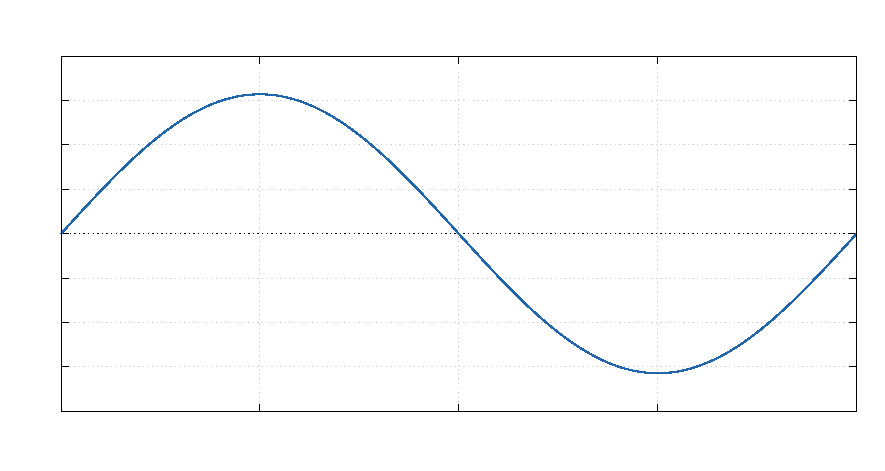
\includegraphics[width={425.00bp},height={226.00bp}]{figures/assignment6_breathing_waveform}}%
    \gplfronttext
  \end{picture}%
\endgroup
}
  \caption{Prescribed sinusoidal inlet flow for the postoperative transient
  simulation. Positive and negative flow denote inspiration and expiration,
  respectively.}
  \label{fig:transient_waveform}
\end{figure}

\begin{table}[htbp]
  \centering
  \caption{Transient postoperative simulation settings.}
  \label{tab:transient_settings}
  \begin{tabular}{@{}ll@{}}
    \toprule
    Parameter & Value \\
    \midrule
    Solver & \texttt{pimpleFoam} \\
    Breathing-cycle duration & \SI{2.0}{\second} \\
    Initial / maximum time step & \SI{1e-5}{\second} / \SI{5e-5}{\second} \\
    Maximum Courant number & 2.0 \\
    Field write interval & \SI{0.02}{\second} \\
    Timing / pilot intervals & \SI{0.05}{\second} / \SI{0.55}{\second} \\
    Simulated cycles & One initially; extend if not periodic \\
    PIMPLE correctors & Up to 3 outer, 2 pressure, 1 non-orthogonal \\
    Outer stopping targets & $2\times10^{-3}$ ($U$), $10^{-2}$ ($p$) \\
    Linear-equation tolerance & $10^{-8}$ ($U$ and $p$) \\
    Parallel decomposition & Scotch, 48 MPI ranks \\
    \bottomrule
  \end{tabular}
\end{table}

% -----------------------------------------------------------------------------
\section{Verification}
\label{sec:verification}

\subsection{Mesh quality}

Table~\ref{tab:mesh_quality} summarises the principal \texttt{checkMesh}
metrics for the four postoperative HXT meshes. All meshes contained one
connected fluid region. A face was counted as severely non-orthogonal when its
non-orthogonality exceeded $70^\circ$.

\begin{table}[htbp]
  \centering
  \caption{Postoperative HXT mesh-quality metrics reported by
  \texttt{checkMesh}. The minimum cell volumes are given after conversion of
  the geometry from millimetres to metres.}
  \label{tab:mesh_quality}
  \resizebox{\textwidth}{!}{%
  \begin{tabular}{@{}lrrrrrr@{}}
    \toprule
    Target size & Max. aspect ratio & Max. non-orthogonality & Severe faces & Max. skewness & Min. volume (\si{\metre\cubed}) & Regions \\
    \midrule
    \SI{0.25}{\milli\metre} & 114.14 & $88.63^\circ$ & 2  & 1.457 & $7.90\times10^{-15}$ & 1 \\
    \SI{0.20}{\milli\metre} & 11.73  & $80.29^\circ$ & 2  & 1.268 & $3.64\times10^{-14}$ & 1 \\
    \SI{0.15}{\milli\metre} & 12.63  & $69.82^\circ$ & 0  & 1.196 & $5.12\times10^{-14}$ & 1 \\
    \SI{0.12}{\milli\metre} & 88.00  & $82.34^\circ$ & 19 & 1.396 & $8.71\times10^{-16}$ & 1 \\
    \bottomrule
  \end{tabular}%
  }
\end{table}

The \SI{0.15}{\milli\metre} mesh had the strongest overall quality: its maximum
non-orthogonality remained below $70^\circ$, it contained no severely
non-orthogonal faces, and it had the lowest maximum skewness of the series. Its
maximum aspect ratio of 12.63 was also substantially lower than those of the
\SI{0.25}{\milli\metre} and \SI{0.12}{\milli\metre} meshes. Refining the target
size did not improve every quality measure monotonically. In particular, the
\SI{0.12}{\milli\metre} mesh introduced 19 severely non-orthogonal faces, a
maximum aspect ratio of 88.00, and the smallest cell volume in the series. This
local deterioration is consistent with its poorer solver convergence and shows
why cell count alone is not a sufficient mesh-selection criterion. Nevertheless,
all four meshes remained single connected domains and their maximum skewness was
below the OpenFOAM internal-cell warning limit of 4. The quality results therefore
support selection of the \SI{0.15}{\milli\metre} mesh for the final analysis.

\subsection{Convergence and mass conservation}

The SIMPLE solution met residual control after 589 iterations. Final initial
residuals were $9.93\times10^{-7}$, $7.57\times10^{-7}$, and
$6.48\times10^{-7}$ for $U_x$, $U_y$, and $U_z$, respectively, and
$4.92\times10^{-6}$ for pressure. These are below the configured criteria of
$10^{-6}$ for velocity and $10^{-5}$ for pressure. Final outlet-flow integration
is still used to verify that

\begin{equation}
  Q_{\mathrm{in}} + \sum_{i=1}^{3} Q_{\mathrm{out},i} \approx 0,
\end{equation}

using a consistent outward-normal sign convention. Report the relative mass
imbalance.

\begin{figure}[htbp]
  \centering
  \resizebox{0.95\textwidth}{!}{\input{figures/assignment4_residuals.tex}}
  \caption{Initial residual evolution for the postoperative steady simulation.
  Dashed and dotted lines indicate the configured velocity and pressure
  convergence criteria. The SIMPLE algorithm stopped at iteration 589 after all
  criteria were satisfied.}
  \label{fig:steady_residuals}
\end{figure}

\subsection{Effect of additional steady iterations}

Assignment 4 requests an assessment of whether 1000 additional iterations alter
an axial-velocity parameter. A fixed centerline-normal section before the
bifurcation is used, and its area-averaged axial velocity is recorded before and
after continuation without reinitialising the solution.

\begin{table}[htbp]
  \centering
  \caption{Sensitivity of the selected axial-velocity monitor to 1000 additional
  steady iterations.}
  \label{tab:additional_iterations}
  \begin{tabular}{@{}lrrr@{}}
    \toprule
    Parameter & Iteration 2000 & Iteration 3000 & Relative change (\%) \\
    \midrule
    Area-averaged axial velocity & [insert] & [insert] & [insert] \\
    \bottomrule
  \end{tabular}
\end{table}

\subsection{Mesh-independence assessment}
\label{sec:mesh_sensitivity}

At least three postoperative mesh levels are preferred so that a trend can be
assessed rather than only a pairwise difference. Each parameter of interest is
plotted against the number of volume elements. For mesh $i$ and the densest mesh
$d$, the Assignment 5 percentage difference is defined as

\begin{equation}
  \delta_{\phi,i} =
  \frac{|\phi_i-\phi_d|}{|\phi_d|}\times 100\%.
  \label{eq:mesh_difference}
\end{equation}

\begin{table}[htbp]
  \centering
  \caption{Mesh-independence comparison.}
  \label{tab:mesh_independence}
  \begin{tabular}{@{}lrrrr@{}}
    \toprule
    Quantity & 0.25 mm & 0.20 mm & 0.15 mm & 0.12 mm \\
    \midrule
    Resistance (Pa/(L/min)) & 15.153 & 16.361 & 17.544 & 17.906 \\
    Peak velocity (m/s) & 9.447 & 9.573 & 9.670 & 9.822 \\
    Right-lung fraction (\%) & 73.664 & 73.619 & 73.686 & 73.397 \\
    Right-superior share (\%) & 15.231 & 15.597 & 16.017 & 16.250 \\
    Solver iterations & 596 & 770 & 1611 & 2000$^*$ \\
    \bottomrule
  \end{tabular}
  \\[2pt]\footnotesize{$^*$Iteration limit reached without satisfying residual control.}
\end{table}

\begin{figure}[htbp]
  \centering
  \resizebox{0.98\textwidth}{!}{% GNUPLOT: LaTeX picture with Postscript
\begingroup
  \makeatletter
  \providecommand\color[2][]{%
    \GenericError{(gnuplot) \space\space\space\@spaces}{%
      Package color not loaded in conjunction with
      terminal option `colourtext'%
    }{See the gnuplot documentation for explanation.%
    }{Either use 'blacktext' in gnuplot or load the package
      color.sty in LaTeX.}%
    \renewcommand\color[2][]{}%
  }%
  \providecommand\includegraphics[2][]{%
    \GenericError{(gnuplot) \space\space\space\@spaces}{%
      Package graphicx or graphics not loaded%
    }{See the gnuplot documentation for explanation.%
    }{The gnuplot epslatex terminal needs graphicx.sty or graphics.sty.}%
    \renewcommand\includegraphics[2][]{}%
  }%
  \providecommand\rotatebox[2]{#2}%
  \@ifundefined{ifGPcolor}{%
    \newif\ifGPcolor
    \GPcolortrue
  }{}%
  \@ifundefined{ifGPblacktext}{%
    \newif\ifGPblacktext
    \GPblacktexttrue
  }{}%
  % define a \g@addto@macro without @ in the name:
  \let\gplgaddtomacro\g@addto@macro
  % define empty templates for all commands taking text:
  \gdef\gplbacktext{}%
  \gdef\gplfronttext{}%
  \makeatother
  \ifGPblacktext
    % no textcolor at all
    \def\colorrgb#1{}%
    \def\colorgray#1{}%
  \else
    % gray or color?
    \ifGPcolor
      \def\colorrgb#1{\color[rgb]{#1}}%
      \def\colorgray#1{\color[gray]{#1}}%
      \expandafter\def\csname LTw\endcsname{\color{white}}%
      \expandafter\def\csname LTb\endcsname{\color{black}}%
      \expandafter\def\csname LTa\endcsname{\color{black}}%
      \expandafter\def\csname LT0\endcsname{\color[rgb]{1,0,0}}%
      \expandafter\def\csname LT1\endcsname{\color[rgb]{0,1,0}}%
      \expandafter\def\csname LT2\endcsname{\color[rgb]{0,0,1}}%
      \expandafter\def\csname LT3\endcsname{\color[rgb]{1,0,1}}%
      \expandafter\def\csname LT4\endcsname{\color[rgb]{0,1,1}}%
      \expandafter\def\csname LT5\endcsname{\color[rgb]{1,1,0}}%
      \expandafter\def\csname LT6\endcsname{\color[rgb]{0,0,0}}%
      \expandafter\def\csname LT7\endcsname{\color[rgb]{1,0.3,0}}%
      \expandafter\def\csname LT8\endcsname{\color[rgb]{0.5,0.5,0.5}}%
    \else
      % gray
      \def\colorrgb#1{\color{black}}%
      \def\colorgray#1{\color[gray]{#1}}%
      \expandafter\def\csname LTw\endcsname{\color{white}}%
      \expandafter\def\csname LTb\endcsname{\color{black}}%
      \expandafter\def\csname LTa\endcsname{\color{black}}%
      \expandafter\def\csname LT0\endcsname{\color{black}}%
      \expandafter\def\csname LT1\endcsname{\color{black}}%
      \expandafter\def\csname LT2\endcsname{\color{black}}%
      \expandafter\def\csname LT3\endcsname{\color{black}}%
      \expandafter\def\csname LT4\endcsname{\color{black}}%
      \expandafter\def\csname LT5\endcsname{\color{black}}%
      \expandafter\def\csname LT6\endcsname{\color{black}}%
      \expandafter\def\csname LT7\endcsname{\color{black}}%
      \expandafter\def\csname LT8\endcsname{\color{black}}%
    \fi
  \fi
    \setlength{\unitlength}{0.0500bp}%
    \ifx\gptboxheight\undefined%
      \newlength{\gptboxheight}%
      \newlength{\gptboxwidth}%
      \newsavebox{\gptboxtext}%
    \fi%
    \setlength{\fboxrule}{0.5pt}%
    \setlength{\fboxsep}{1pt}%
    \definecolor{tbcol}{rgb}{1,1,1}%
\begin{picture}(9060.00,7360.00)%
    \gplgaddtomacro\gplbacktext{%
      \csname LTb\endcsname%%
      \put(598,4176){\makebox(0,0)[r]{\strut{}$15$}}%
      \csname LTb\endcsname%%
      \put(598,4624){\makebox(0,0)[r]{\strut{}$15.5$}}%
      \csname LTb\endcsname%%
      \put(598,5072){\makebox(0,0)[r]{\strut{}$16$}}%
      \csname LTb\endcsname%%
      \put(598,5520){\makebox(0,0)[r]{\strut{}$16.5$}}%
      \csname LTb\endcsname%%
      \put(598,5968){\makebox(0,0)[r]{\strut{}$17$}}%
      \csname LTb\endcsname%%
      \put(598,6416){\makebox(0,0)[r]{\strut{}$17.5$}}%
      \csname LTb\endcsname%%
      \put(598,6864){\makebox(0,0)[r]{\strut{}$18$}}%
      \csname LTb\endcsname%%
      \put(679,4018){\makebox(0,0){\strut{}0.0$\times10^{0}$}}%
      \csname LTb\endcsname%%
      \put(1129,4018){\makebox(0,0){\strut{}2.0$\times10^{5}$}}%
      \csname LTb\endcsname%%
      \put(1579,4018){\makebox(0,0){\strut{}4.0$\times10^{5}$}}%
      \csname LTb\endcsname%%
      \put(2029,4018){\makebox(0,0){\strut{}6.0$\times10^{5}$}}%
      \csname LTb\endcsname%%
      \put(2479,4018){\makebox(0,0){\strut{}8.0$\times10^{5}$}}%
      \csname LTb\endcsname%%
      \put(2929,4018){\makebox(0,0){\strut{}1.0$\times10^{6}$}}%
      \csname LTb\endcsname%%
      \put(3379,4018){\makebox(0,0){\strut{}1.2$\times10^{6}$}}%
      \csname LTb\endcsname%%
      \put(3829,4018){\makebox(0,0){\strut{}1.4$\times10^{6}$}}%
      \csname LTb\endcsname%%
      \put(4279,4018){\makebox(0,0){\strut{}1.6$\times10^{6}$}}%
    }%
    \gplgaddtomacro\gplfronttext{%
      \csname LTb\endcsname%%
      \put(139,5520){\rotatebox{-270.00}{\makebox(0,0){\strut{}Resistance (Pa/(L/min))}}}%
      \csname LTb\endcsname%%
      \put(2479,3780){\makebox(0,0){\strut{}Number of volume cells}}%
      \csname LTb\endcsname%%
      \put(2479,7102){\makebox(0,0){\strut{}Resistance (Pa/(L/min))}}%
    }%
    \gplgaddtomacro\gplbacktext{%
      \csname LTb\endcsname%%
      \put(5199,4176){\makebox(0,0)[r]{\strut{}$73.35$}}%
      \csname LTb\endcsname%%
      \put(5199,4560){\makebox(0,0)[r]{\strut{}$73.4$}}%
      \csname LTb\endcsname%%
      \put(5199,4944){\makebox(0,0)[r]{\strut{}$73.45$}}%
      \csname LTb\endcsname%%
      \put(5199,5328){\makebox(0,0)[r]{\strut{}$73.5$}}%
      \csname LTb\endcsname%%
      \put(5199,5712){\makebox(0,0)[r]{\strut{}$73.55$}}%
      \csname LTb\endcsname%%
      \put(5199,6096){\makebox(0,0)[r]{\strut{}$73.6$}}%
      \csname LTb\endcsname%%
      \put(5199,6480){\makebox(0,0)[r]{\strut{}$73.65$}}%
      \csname LTb\endcsname%%
      \put(5199,6864){\makebox(0,0)[r]{\strut{}$73.7$}}%
      \csname LTb\endcsname%%
      \put(5279,4018){\makebox(0,0){\strut{}0.0$\times10^{0}$}}%
      \csname LTb\endcsname%%
      \put(5719,4018){\makebox(0,0){\strut{}2.0$\times10^{5}$}}%
      \csname LTb\endcsname%%
      \put(6159,4018){\makebox(0,0){\strut{}4.0$\times10^{5}$}}%
      \csname LTb\endcsname%%
      \put(6599,4018){\makebox(0,0){\strut{}6.0$\times10^{5}$}}%
      \csname LTb\endcsname%%
      \put(7039,4018){\makebox(0,0){\strut{}8.0$\times10^{5}$}}%
      \csname LTb\endcsname%%
      \put(7479,4018){\makebox(0,0){\strut{}1.0$\times10^{6}$}}%
      \csname LTb\endcsname%%
      \put(7919,4018){\makebox(0,0){\strut{}1.2$\times10^{6}$}}%
      \csname LTb\endcsname%%
      \put(8359,4018){\makebox(0,0){\strut{}1.4$\times10^{6}$}}%
      \csname LTb\endcsname%%
      \put(8799,4018){\makebox(0,0){\strut{}1.6$\times10^{6}$}}%
    }%
    \gplgaddtomacro\gplfronttext{%
      \csname LTb\endcsname%%
      \put(4659,5520){\rotatebox{-270.00}{\makebox(0,0){\strut{}Right-lung flow fraction (\%)}}}%
      \csname LTb\endcsname%%
      \put(7039,3780){\makebox(0,0){\strut{}Number of volume cells}}%
      \csname LTb\endcsname%%
      \put(7039,7102){\makebox(0,0){\strut{}Right-lung flow fraction (\%)}}%
    }%
    \gplgaddtomacro\gplbacktext{%
      \csname LTb\endcsname%%
      \put(598,506){\makebox(0,0)[r]{\strut{}$15.2$}}%
      \csname LTb\endcsname%%
      \put(598,954){\makebox(0,0)[r]{\strut{}$15.4$}}%
      \csname LTb\endcsname%%
      \put(598,1402){\makebox(0,0)[r]{\strut{}$15.6$}}%
      \csname LTb\endcsname%%
      \put(598,1850){\makebox(0,0)[r]{\strut{}$15.8$}}%
      \csname LTb\endcsname%%
      \put(598,2298){\makebox(0,0)[r]{\strut{}$16$}}%
      \csname LTb\endcsname%%
      \put(598,2746){\makebox(0,0)[r]{\strut{}$16.2$}}%
      \csname LTb\endcsname%%
      \put(598,3194){\makebox(0,0)[r]{\strut{}$16.4$}}%
      \csname LTb\endcsname%%
      \put(679,348){\makebox(0,0){\strut{}0.0$\times10^{0}$}}%
      \csname LTb\endcsname%%
      \put(1129,348){\makebox(0,0){\strut{}2.0$\times10^{5}$}}%
      \csname LTb\endcsname%%
      \put(1579,348){\makebox(0,0){\strut{}4.0$\times10^{5}$}}%
      \csname LTb\endcsname%%
      \put(2029,348){\makebox(0,0){\strut{}6.0$\times10^{5}$}}%
      \csname LTb\endcsname%%
      \put(2479,348){\makebox(0,0){\strut{}8.0$\times10^{5}$}}%
      \csname LTb\endcsname%%
      \put(2929,348){\makebox(0,0){\strut{}1.0$\times10^{6}$}}%
      \csname LTb\endcsname%%
      \put(3379,348){\makebox(0,0){\strut{}1.2$\times10^{6}$}}%
      \csname LTb\endcsname%%
      \put(3829,348){\makebox(0,0){\strut{}1.4$\times10^{6}$}}%
      \csname LTb\endcsname%%
      \put(4279,348){\makebox(0,0){\strut{}1.6$\times10^{6}$}}%
    }%
    \gplgaddtomacro\gplfronttext{%
      \csname LTb\endcsname%%
      \put(139,1850){\rotatebox{-270.00}{\makebox(0,0){\strut{}Right-superior share of right flow (\%)}}}%
      \csname LTb\endcsname%%
      \put(2479,110){\makebox(0,0){\strut{}Number of volume cells}}%
      \csname LTb\endcsname%%
      \put(2479,3432){\makebox(0,0){\strut{}Right-superior share of right flow (\%)}}%
    }%
    \gplgaddtomacro\gplbacktext{%
      \csname LTb\endcsname%%
      \put(5118,506){\makebox(0,0)[r]{\strut{}$9.4$}}%
      \csname LTb\endcsname%%
      \put(5118,805){\makebox(0,0)[r]{\strut{}$9.45$}}%
      \csname LTb\endcsname%%
      \put(5118,1104){\makebox(0,0)[r]{\strut{}$9.5$}}%
      \csname LTb\endcsname%%
      \put(5118,1402){\makebox(0,0)[r]{\strut{}$9.55$}}%
      \csname LTb\endcsname%%
      \put(5118,1701){\makebox(0,0)[r]{\strut{}$9.6$}}%
      \csname LTb\endcsname%%
      \put(5118,2000){\makebox(0,0)[r]{\strut{}$9.65$}}%
      \csname LTb\endcsname%%
      \put(5118,2298){\makebox(0,0)[r]{\strut{}$9.7$}}%
      \csname LTb\endcsname%%
      \put(5118,2597){\makebox(0,0)[r]{\strut{}$9.75$}}%
      \csname LTb\endcsname%%
      \put(5118,2896){\makebox(0,0)[r]{\strut{}$9.8$}}%
      \csname LTb\endcsname%%
      \put(5118,3194){\makebox(0,0)[r]{\strut{}$9.85$}}%
      \csname LTb\endcsname%%
      \put(5199,348){\makebox(0,0){\strut{}0.0$\times10^{0}$}}%
      \csname LTb\endcsname%%
      \put(5649,348){\makebox(0,0){\strut{}2.0$\times10^{5}$}}%
      \csname LTb\endcsname%%
      \put(6099,348){\makebox(0,0){\strut{}4.0$\times10^{5}$}}%
      \csname LTb\endcsname%%
      \put(6549,348){\makebox(0,0){\strut{}6.0$\times10^{5}$}}%
      \csname LTb\endcsname%%
      \put(6999,348){\makebox(0,0){\strut{}8.0$\times10^{5}$}}%
      \csname LTb\endcsname%%
      \put(7449,348){\makebox(0,0){\strut{}1.0$\times10^{6}$}}%
      \csname LTb\endcsname%%
      \put(7899,348){\makebox(0,0){\strut{}1.2$\times10^{6}$}}%
      \csname LTb\endcsname%%
      \put(8349,348){\makebox(0,0){\strut{}1.4$\times10^{6}$}}%
      \csname LTb\endcsname%%
      \put(8799,348){\makebox(0,0){\strut{}1.6$\times10^{6}$}}%
    }%
    \gplgaddtomacro\gplfronttext{%
      \csname LTb\endcsname%%
      \put(4659,1850){\rotatebox{-270.00}{\makebox(0,0){\strut{}Matched-section peak velocity (m/s)}}}%
      \csname LTb\endcsname%%
      \put(6999,110){\makebox(0,0){\strut{}Number of volume cells}}%
      \csname LTb\endcsname%%
      \put(6999,3432){\makebox(0,0){\strut{}Matched-section peak velocity (m/s)}}%
    }%
    \gplbacktext
    \put(0,0){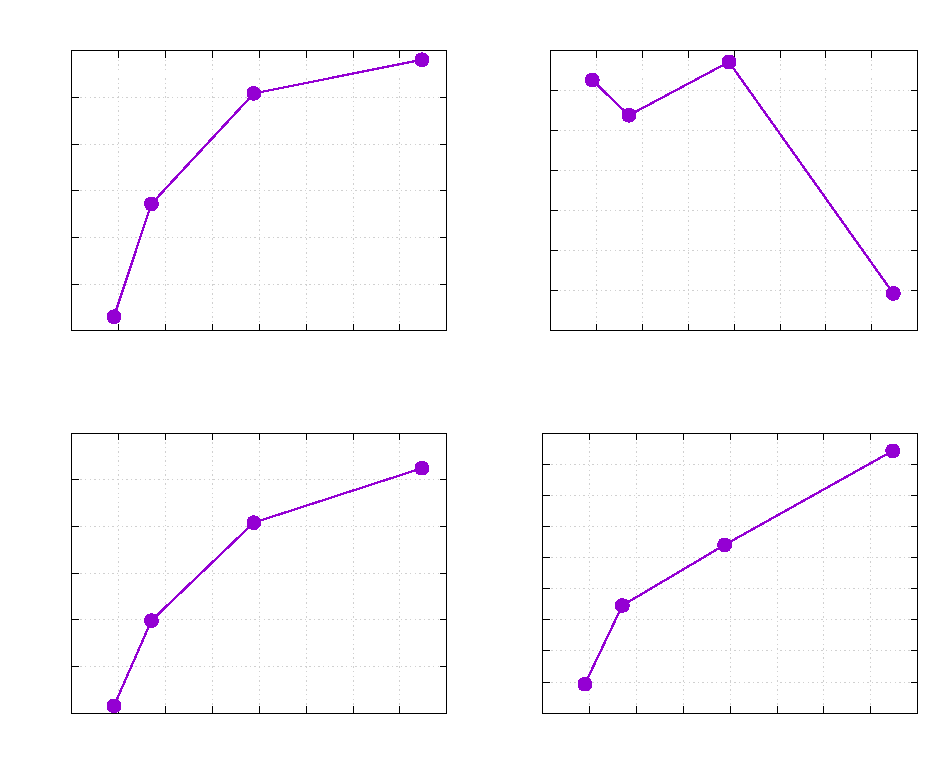
\includegraphics[width={453.00bp},height={368.00bp}]{figures/assignment5_mesh_metrics}}%
    \gplfronttext
  \end{picture}%
\endgroup
}
  \caption{Postoperative mesh-sensitivity metrics as functions of actual volume
  cell count. All meshes use identical geometry, boundary conditions, sampling
  planes, and HXT tetrahedral meshing strategy.}
  \label{fig:mesh_sensitivity}
\end{figure}

\begin{figure}[htbp]
  \centering
  \resizebox{0.98\textwidth}{!}{% GNUPLOT: LaTeX picture with Postscript
\begingroup
  \makeatletter
  \providecommand\color[2][]{%
    \GenericError{(gnuplot) \space\space\space\@spaces}{%
      Package color not loaded in conjunction with
      terminal option `colourtext'%
    }{See the gnuplot documentation for explanation.%
    }{Either use 'blacktext' in gnuplot or load the package
      color.sty in LaTeX.}%
    \renewcommand\color[2][]{}%
  }%
  \providecommand\includegraphics[2][]{%
    \GenericError{(gnuplot) \space\space\space\@spaces}{%
      Package graphicx or graphics not loaded%
    }{See the gnuplot documentation for explanation.%
    }{The gnuplot epslatex terminal needs graphicx.sty or graphics.sty.}%
    \renewcommand\includegraphics[2][]{}%
  }%
  \providecommand\rotatebox[2]{#2}%
  \@ifundefined{ifGPcolor}{%
    \newif\ifGPcolor
    \GPcolortrue
  }{}%
  \@ifundefined{ifGPblacktext}{%
    \newif\ifGPblacktext
    \GPblacktexttrue
  }{}%
  % define a \g@addto@macro without @ in the name:
  \let\gplgaddtomacro\g@addto@macro
  % define empty templates for all commands taking text:
  \gdef\gplbacktext{}%
  \gdef\gplfronttext{}%
  \makeatother
  \ifGPblacktext
    % no textcolor at all
    \def\colorrgb#1{}%
    \def\colorgray#1{}%
  \else
    % gray or color?
    \ifGPcolor
      \def\colorrgb#1{\color[rgb]{#1}}%
      \def\colorgray#1{\color[gray]{#1}}%
      \expandafter\def\csname LTw\endcsname{\color{white}}%
      \expandafter\def\csname LTb\endcsname{\color{black}}%
      \expandafter\def\csname LTa\endcsname{\color{black}}%
      \expandafter\def\csname LT0\endcsname{\color[rgb]{1,0,0}}%
      \expandafter\def\csname LT1\endcsname{\color[rgb]{0,1,0}}%
      \expandafter\def\csname LT2\endcsname{\color[rgb]{0,0,1}}%
      \expandafter\def\csname LT3\endcsname{\color[rgb]{1,0,1}}%
      \expandafter\def\csname LT4\endcsname{\color[rgb]{0,1,1}}%
      \expandafter\def\csname LT5\endcsname{\color[rgb]{1,1,0}}%
      \expandafter\def\csname LT6\endcsname{\color[rgb]{0,0,0}}%
      \expandafter\def\csname LT7\endcsname{\color[rgb]{1,0.3,0}}%
      \expandafter\def\csname LT8\endcsname{\color[rgb]{0.5,0.5,0.5}}%
    \else
      % gray
      \def\colorrgb#1{\color{black}}%
      \def\colorgray#1{\color[gray]{#1}}%
      \expandafter\def\csname LTw\endcsname{\color{white}}%
      \expandafter\def\csname LTb\endcsname{\color{black}}%
      \expandafter\def\csname LTa\endcsname{\color{black}}%
      \expandafter\def\csname LT0\endcsname{\color{black}}%
      \expandafter\def\csname LT1\endcsname{\color{black}}%
      \expandafter\def\csname LT2\endcsname{\color{black}}%
      \expandafter\def\csname LT3\endcsname{\color{black}}%
      \expandafter\def\csname LT4\endcsname{\color{black}}%
      \expandafter\def\csname LT5\endcsname{\color{black}}%
      \expandafter\def\csname LT6\endcsname{\color{black}}%
      \expandafter\def\csname LT7\endcsname{\color{black}}%
      \expandafter\def\csname LT8\endcsname{\color{black}}%
    \fi
  \fi
    \setlength{\unitlength}{0.0500bp}%
    \ifx\gptboxheight\undefined%
      \newlength{\gptboxheight}%
      \newlength{\gptboxwidth}%
      \newsavebox{\gptboxtext}%
    \fi%
    \setlength{\fboxrule}{0.5pt}%
    \setlength{\fboxsep}{1pt}%
    \definecolor{tbcol}{rgb}{1,1,1}%
\begin{picture}(9060.00,7360.00)%
    \gplgaddtomacro\gplbacktext{%
      \csname LTb\endcsname%%
      \put(438,4176){\makebox(0,0)[r]{\strut{}$0$}}%
      \csname LTb\endcsname%%
      \put(438,4512){\makebox(0,0)[r]{\strut{}$2$}}%
      \csname LTb\endcsname%%
      \put(438,4848){\makebox(0,0)[r]{\strut{}$4$}}%
      \csname LTb\endcsname%%
      \put(438,5184){\makebox(0,0)[r]{\strut{}$6$}}%
      \csname LTb\endcsname%%
      \put(438,5520){\makebox(0,0)[r]{\strut{}$8$}}%
      \csname LTb\endcsname%%
      \put(438,5856){\makebox(0,0)[r]{\strut{}$10$}}%
      \csname LTb\endcsname%%
      \put(438,6192){\makebox(0,0)[r]{\strut{}$12$}}%
      \csname LTb\endcsname%%
      \put(438,6528){\makebox(0,0)[r]{\strut{}$14$}}%
      \csname LTb\endcsname%%
      \put(438,6864){\makebox(0,0)[r]{\strut{}$16$}}%
      \csname LTb\endcsname%%
      \put(518,4018){\makebox(0,0){\strut{}0.0$\times10^{0}$}}%
      \csname LTb\endcsname%%
      \put(988,4018){\makebox(0,0){\strut{}2.0$\times10^{5}$}}%
      \csname LTb\endcsname%%
      \put(1459,4018){\makebox(0,0){\strut{}4.0$\times10^{5}$}}%
      \csname LTb\endcsname%%
      \put(1929,4018){\makebox(0,0){\strut{}6.0$\times10^{5}$}}%
      \csname LTb\endcsname%%
      \put(2399,4018){\makebox(0,0){\strut{}8.0$\times10^{5}$}}%
      \csname LTb\endcsname%%
      \put(2869,4018){\makebox(0,0){\strut{}1.0$\times10^{6}$}}%
      \csname LTb\endcsname%%
      \put(3339,4018){\makebox(0,0){\strut{}1.2$\times10^{6}$}}%
      \csname LTb\endcsname%%
      \put(3809,4018){\makebox(0,0){\strut{}1.4$\times10^{6}$}}%
      \csname LTb\endcsname%%
      \put(4279,4018){\makebox(0,0){\strut{}1.6$\times10^{6}$}}%
    }%
    \gplgaddtomacro\gplfronttext{%
      \csname LTb\endcsname%%
      \put(139,5520){\rotatebox{-270.00}{\makebox(0,0){\strut{}Difference from finest mesh (\%)}}}%
      \csname LTb\endcsname%%
      \put(2399,3780){\makebox(0,0){\strut{}Number of volume cells}}%
      \csname LTb\endcsname%%
      \put(2399,7102){\makebox(0,0){\strut{}Resistance (Pa/(L/min))}}%
    }%
    \gplgaddtomacro\gplbacktext{%
      \csname LTb\endcsname%%
      \put(5118,4176){\makebox(0,0)[r]{\strut{}$0$}}%
      \csname LTb\endcsname%%
      \put(5118,4512){\makebox(0,0)[r]{\strut{}$0.05$}}%
      \csname LTb\endcsname%%
      \put(5118,4848){\makebox(0,0)[r]{\strut{}$0.1$}}%
      \csname LTb\endcsname%%
      \put(5118,5184){\makebox(0,0)[r]{\strut{}$0.15$}}%
      \csname LTb\endcsname%%
      \put(5118,5520){\makebox(0,0)[r]{\strut{}$0.2$}}%
      \csname LTb\endcsname%%
      \put(5118,5856){\makebox(0,0)[r]{\strut{}$0.25$}}%
      \csname LTb\endcsname%%
      \put(5118,6192){\makebox(0,0)[r]{\strut{}$0.3$}}%
      \csname LTb\endcsname%%
      \put(5118,6528){\makebox(0,0)[r]{\strut{}$0.35$}}%
      \csname LTb\endcsname%%
      \put(5118,6864){\makebox(0,0)[r]{\strut{}$0.4$}}%
      \csname LTb\endcsname%%
      \put(5199,4018){\makebox(0,0){\strut{}0.0$\times10^{0}$}}%
      \csname LTb\endcsname%%
      \put(5649,4018){\makebox(0,0){\strut{}2.0$\times10^{5}$}}%
      \csname LTb\endcsname%%
      \put(6099,4018){\makebox(0,0){\strut{}4.0$\times10^{5}$}}%
      \csname LTb\endcsname%%
      \put(6549,4018){\makebox(0,0){\strut{}6.0$\times10^{5}$}}%
      \csname LTb\endcsname%%
      \put(6999,4018){\makebox(0,0){\strut{}8.0$\times10^{5}$}}%
      \csname LTb\endcsname%%
      \put(7449,4018){\makebox(0,0){\strut{}1.0$\times10^{6}$}}%
      \csname LTb\endcsname%%
      \put(7899,4018){\makebox(0,0){\strut{}1.2$\times10^{6}$}}%
      \csname LTb\endcsname%%
      \put(8349,4018){\makebox(0,0){\strut{}1.4$\times10^{6}$}}%
      \csname LTb\endcsname%%
      \put(8799,4018){\makebox(0,0){\strut{}1.6$\times10^{6}$}}%
    }%
    \gplgaddtomacro\gplfronttext{%
      \csname LTb\endcsname%%
      \put(4659,5520){\rotatebox{-270.00}{\makebox(0,0){\strut{}Difference from finest mesh (\%)}}}%
      \csname LTb\endcsname%%
      \put(6999,3780){\makebox(0,0){\strut{}Number of volume cells}}%
      \csname LTb\endcsname%%
      \put(6999,7102){\makebox(0,0){\strut{}Right-lung flow fraction (\%)}}%
    }%
    \gplgaddtomacro\gplbacktext{%
      \csname LTb\endcsname%%
      \put(358,506){\makebox(0,0)[r]{\strut{}$0$}}%
      \csname LTb\endcsname%%
      \put(358,890){\makebox(0,0)[r]{\strut{}$1$}}%
      \csname LTb\endcsname%%
      \put(358,1274){\makebox(0,0)[r]{\strut{}$2$}}%
      \csname LTb\endcsname%%
      \put(358,1658){\makebox(0,0)[r]{\strut{}$3$}}%
      \csname LTb\endcsname%%
      \put(358,2042){\makebox(0,0)[r]{\strut{}$4$}}%
      \csname LTb\endcsname%%
      \put(358,2426){\makebox(0,0)[r]{\strut{}$5$}}%
      \csname LTb\endcsname%%
      \put(358,2810){\makebox(0,0)[r]{\strut{}$6$}}%
      \csname LTb\endcsname%%
      \put(358,3194){\makebox(0,0)[r]{\strut{}$7$}}%
      \csname LTb\endcsname%%
      \put(438,348){\makebox(0,0){\strut{}0.0$\times10^{0}$}}%
      \csname LTb\endcsname%%
      \put(918,348){\makebox(0,0){\strut{}2.0$\times10^{5}$}}%
      \csname LTb\endcsname%%
      \put(1398,348){\makebox(0,0){\strut{}4.0$\times10^{5}$}}%
      \csname LTb\endcsname%%
      \put(1879,348){\makebox(0,0){\strut{}6.0$\times10^{5}$}}%
      \csname LTb\endcsname%%
      \put(2359,348){\makebox(0,0){\strut{}8.0$\times10^{5}$}}%
      \csname LTb\endcsname%%
      \put(2839,348){\makebox(0,0){\strut{}1.0$\times10^{6}$}}%
      \csname LTb\endcsname%%
      \put(3319,348){\makebox(0,0){\strut{}1.2$\times10^{6}$}}%
      \csname LTb\endcsname%%
      \put(3799,348){\makebox(0,0){\strut{}1.4$\times10^{6}$}}%
      \csname LTb\endcsname%%
      \put(4279,348){\makebox(0,0){\strut{}1.6$\times10^{6}$}}%
    }%
    \gplgaddtomacro\gplfronttext{%
      \csname LTb\endcsname%%
      \put(139,1850){\rotatebox{-270.00}{\makebox(0,0){\strut{}Difference from finest mesh (\%)}}}%
      \csname LTb\endcsname%%
      \put(2359,110){\makebox(0,0){\strut{}Number of volume cells}}%
      \csname LTb\endcsname%%
      \put(2359,3432){\makebox(0,0){\strut{}Right-superior share of right flow (\%)}}%
    }%
    \gplgaddtomacro\gplbacktext{%
      \csname LTb\endcsname%%
      \put(5038,506){\makebox(0,0)[r]{\strut{}$0$}}%
      \csname LTb\endcsname%%
      \put(5038,842){\makebox(0,0)[r]{\strut{}$0.5$}}%
      \csname LTb\endcsname%%
      \put(5038,1178){\makebox(0,0)[r]{\strut{}$1$}}%
      \csname LTb\endcsname%%
      \put(5038,1514){\makebox(0,0)[r]{\strut{}$1.5$}}%
      \csname LTb\endcsname%%
      \put(5038,1850){\makebox(0,0)[r]{\strut{}$2$}}%
      \csname LTb\endcsname%%
      \put(5038,2186){\makebox(0,0)[r]{\strut{}$2.5$}}%
      \csname LTb\endcsname%%
      \put(5038,2522){\makebox(0,0)[r]{\strut{}$3$}}%
      \csname LTb\endcsname%%
      \put(5038,2858){\makebox(0,0)[r]{\strut{}$3.5$}}%
      \csname LTb\endcsname%%
      \put(5038,3194){\makebox(0,0)[r]{\strut{}$4$}}%
      \csname LTb\endcsname%%
      \put(5118,348){\makebox(0,0){\strut{}0.0$\times10^{0}$}}%
      \csname LTb\endcsname%%
      \put(5579,348){\makebox(0,0){\strut{}2.0$\times10^{5}$}}%
      \csname LTb\endcsname%%
      \put(6039,348){\makebox(0,0){\strut{}4.0$\times10^{5}$}}%
      \csname LTb\endcsname%%
      \put(6499,348){\makebox(0,0){\strut{}6.0$\times10^{5}$}}%
      \csname LTb\endcsname%%
      \put(6959,348){\makebox(0,0){\strut{}8.0$\times10^{5}$}}%
      \csname LTb\endcsname%%
      \put(7419,348){\makebox(0,0){\strut{}1.0$\times10^{6}$}}%
      \csname LTb\endcsname%%
      \put(7879,348){\makebox(0,0){\strut{}1.2$\times10^{6}$}}%
      \csname LTb\endcsname%%
      \put(8339,348){\makebox(0,0){\strut{}1.4$\times10^{6}$}}%
      \csname LTb\endcsname%%
      \put(8799,348){\makebox(0,0){\strut{}1.6$\times10^{6}$}}%
    }%
    \gplgaddtomacro\gplfronttext{%
      \csname LTb\endcsname%%
      \put(4659,1850){\rotatebox{-270.00}{\makebox(0,0){\strut{}Difference from finest mesh (\%)}}}%
      \csname LTb\endcsname%%
      \put(6959,110){\makebox(0,0){\strut{}Number of volume cells}}%
      \csname LTb\endcsname%%
      \put(6959,3432){\makebox(0,0){\strut{}Matched-section peak velocity (m/s)}}%
    }%
    \gplbacktext
    \put(0,0){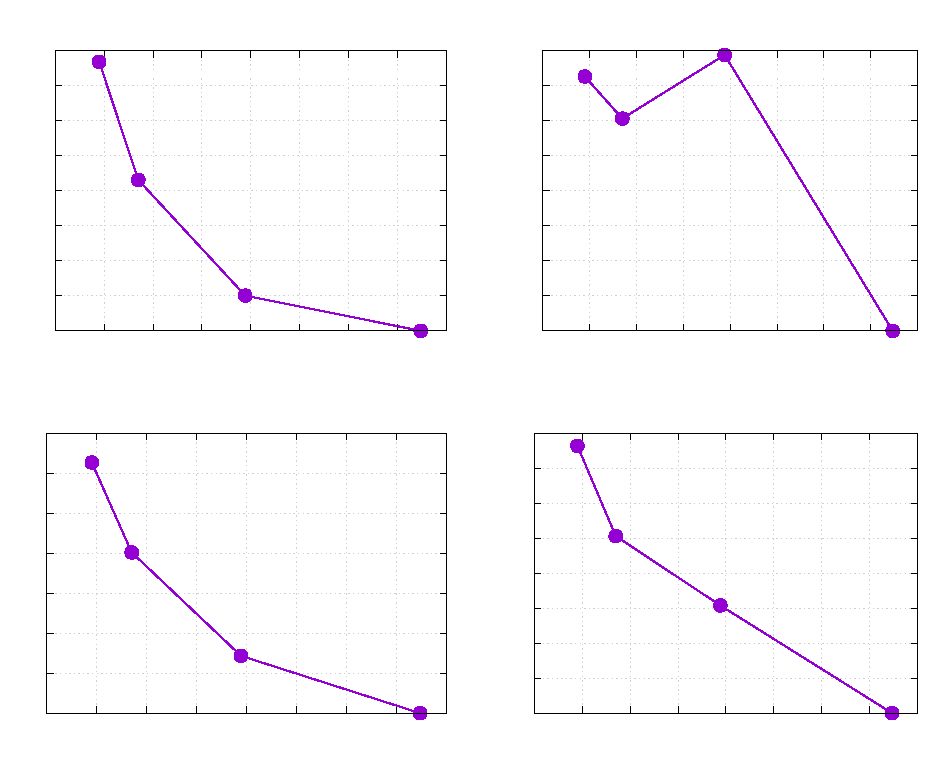
\includegraphics[width={453.00bp},height={368.00bp}]{figures/assignment5_mesh_differences}}%
    \gplfronttext
  \end{picture}%
\endgroup
}
  \caption{Absolute relative differences from the densest 0.12 mm mesh,
  calculated as $|\phi_i-\phi_d|/|\phi_d|\times100\%$. The densest case reached
  its 2000-iteration limit without satisfying residual control and is therefore
  a requested comparison rather than an accepted truth solution.}
  \label{fig:mesh_sensitivity_differences}
\end{figure}

% -----------------------------------------------------------------------------
\section{Results}
\label{sec:results}

\subsection{Velocity field}

At the converged postoperative solution, velocity vectors accelerate through the
narrow distal trachea and divide at the carina. The fixed matched section has an
area-averaged axial velocity of \SI{6.53}{\metre\per\second} and a sectional
peak magnitude of \SI{9.25}{\metre\per\second}. The vectors also show the
unequal right/left flow division quantified from patch fluxes.

\begin{figure}[htbp]
  \centering
  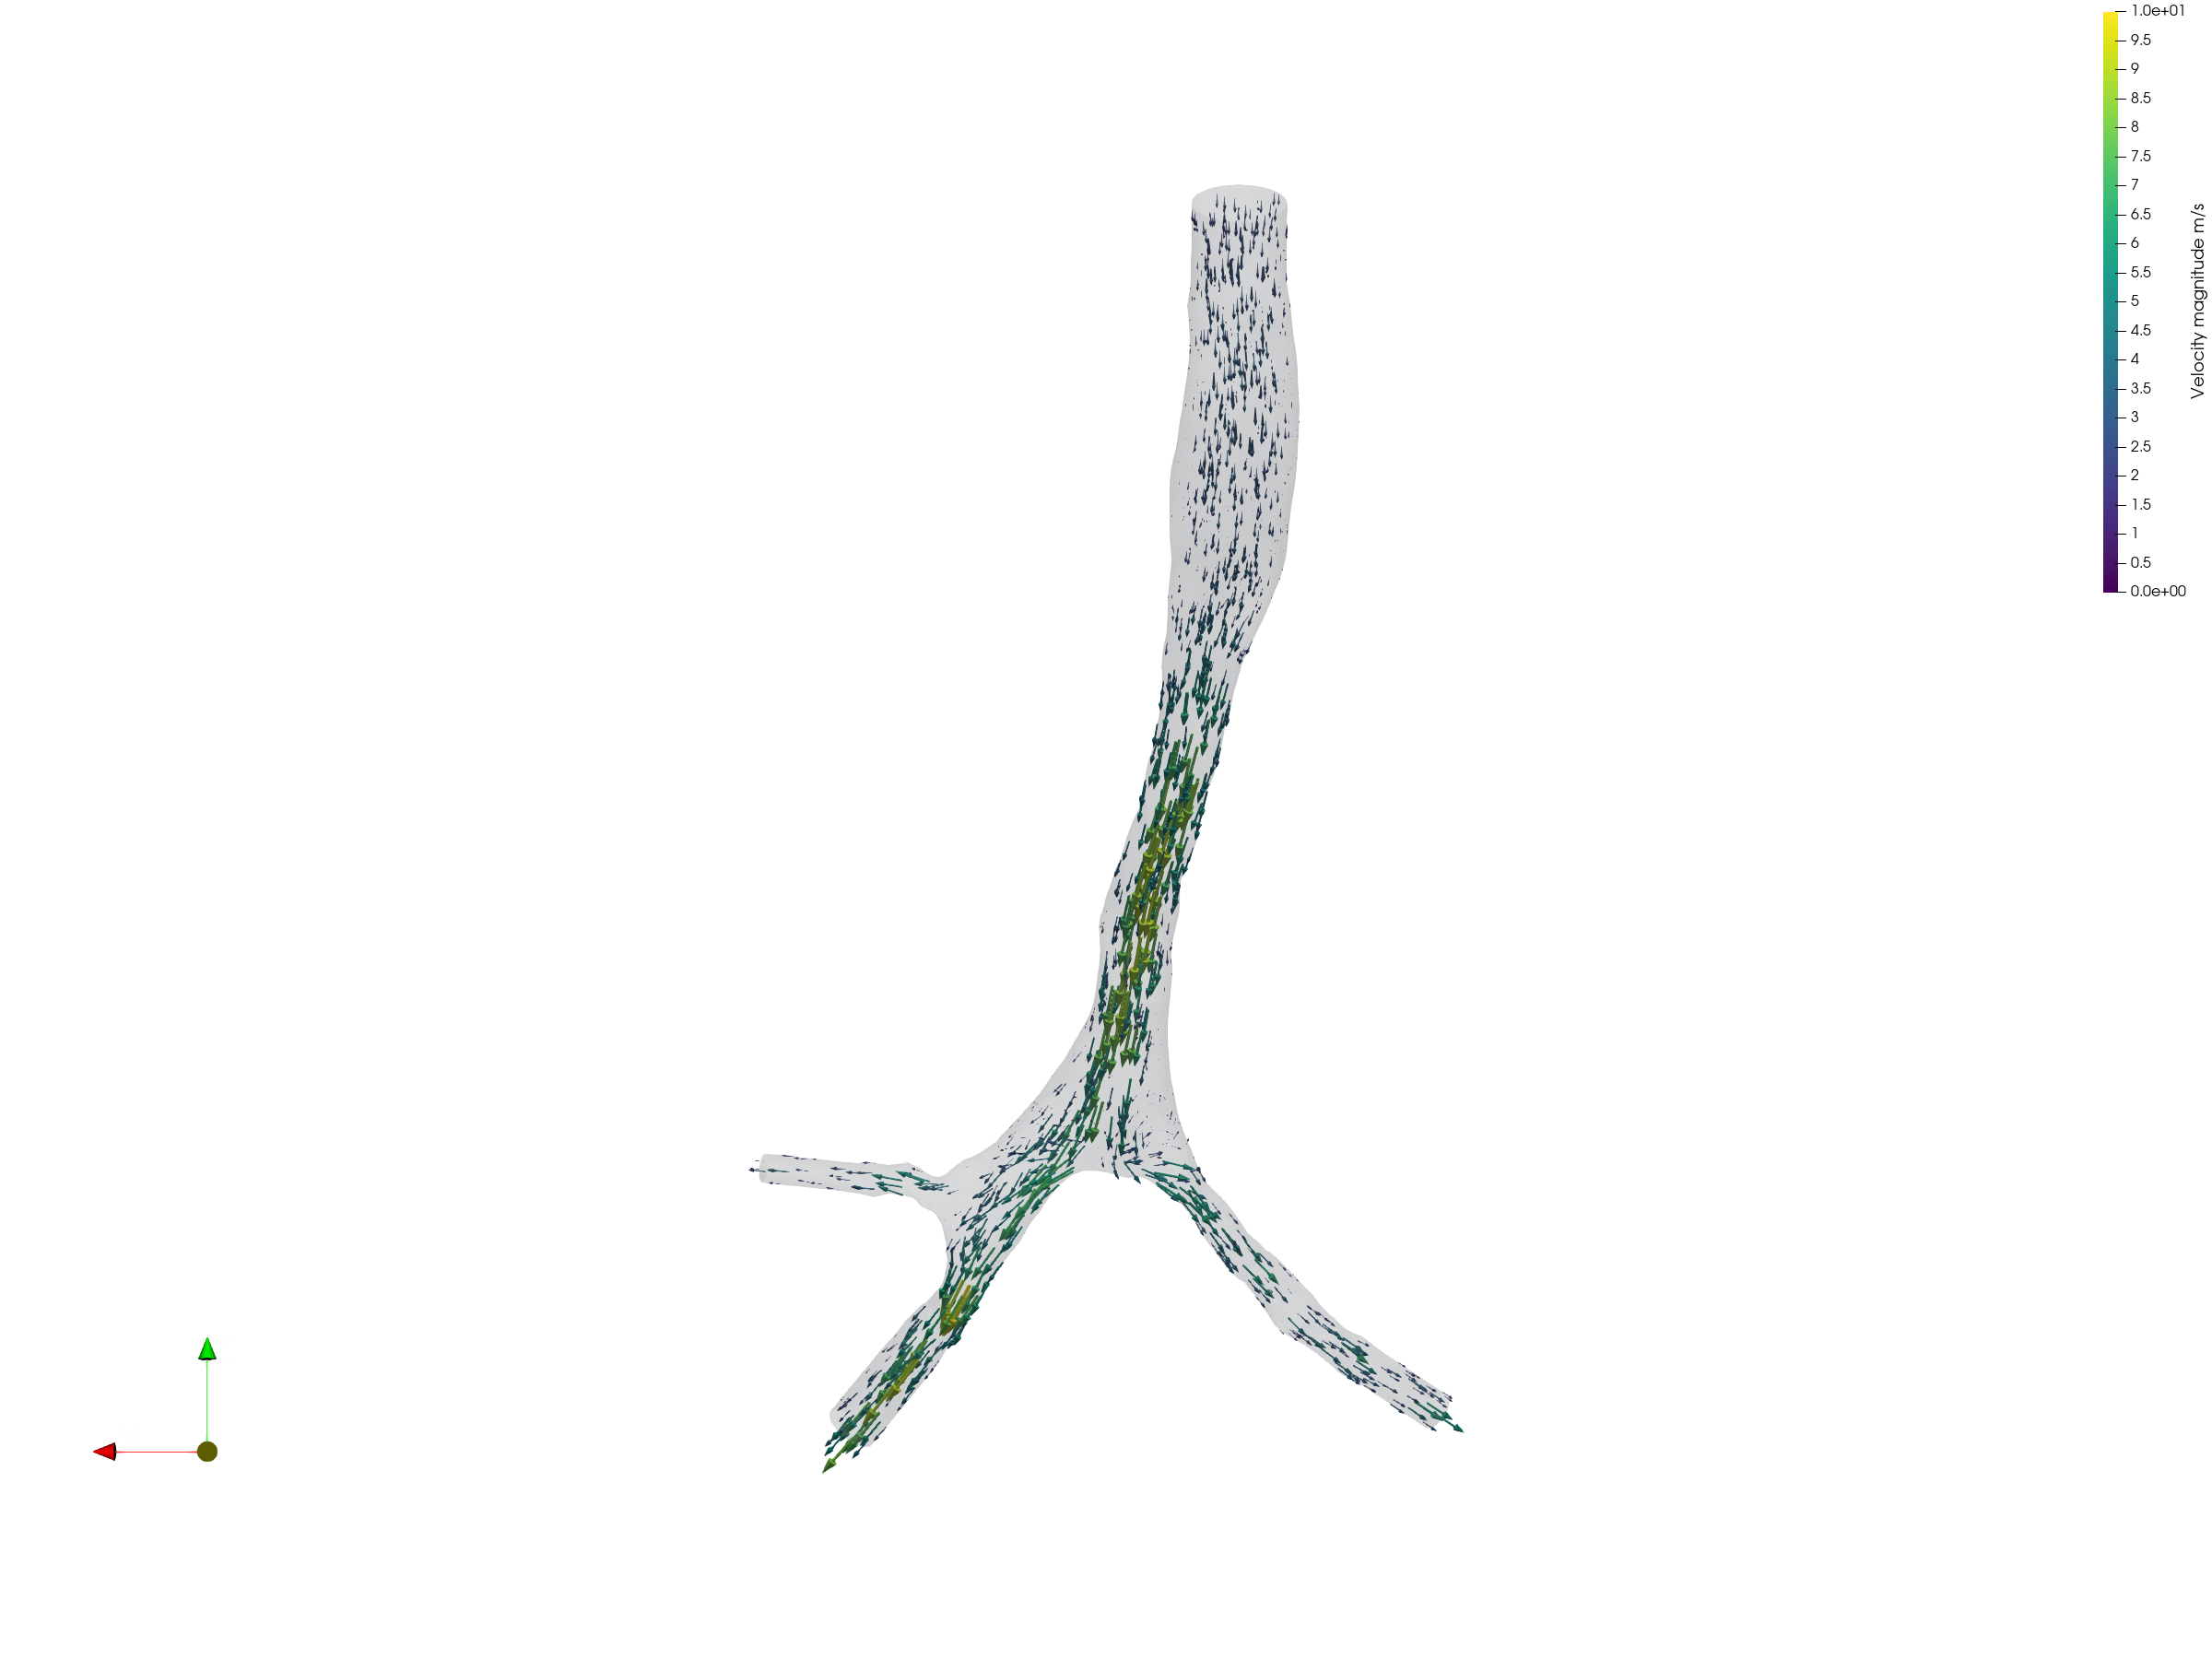
\includegraphics[width=0.92\textwidth]{assignment4_velocity_vectors.png}
  \caption{Postoperative velocity-vector field at the converged steady solution
  (iteration 589). Arrow direction represents local flow direction; arrow colour
  represents velocity magnitude on a fixed \SIrange{0}{10}{\metre\per\second}
  scale. The airway surface is shown semi-transparently for anatomical context.}
  \label{fig:velocity}
\end{figure}

\subsection{Pressure distribution}

Pressure is reported relative to the zero-gauge-pressure outlets and converted
from OpenFOAM kinematic pressure using $P=\rho p$ with
$\rho=\SI{1.204}{\kilogram\per\metre\cubed}$. Pressure decreases from the
tracheal inlet toward the outlets. Along the mapped centerline interval it falls
from approximately \SI{65.1}{\pascal} to \SI{34.1}{\pascal}, with a local
minimum followed by partial recovery. The resistance calculation uses
area-averaged plane pressures rather than centerline point samples.

\begin{figure}[htbp]
  \centering
  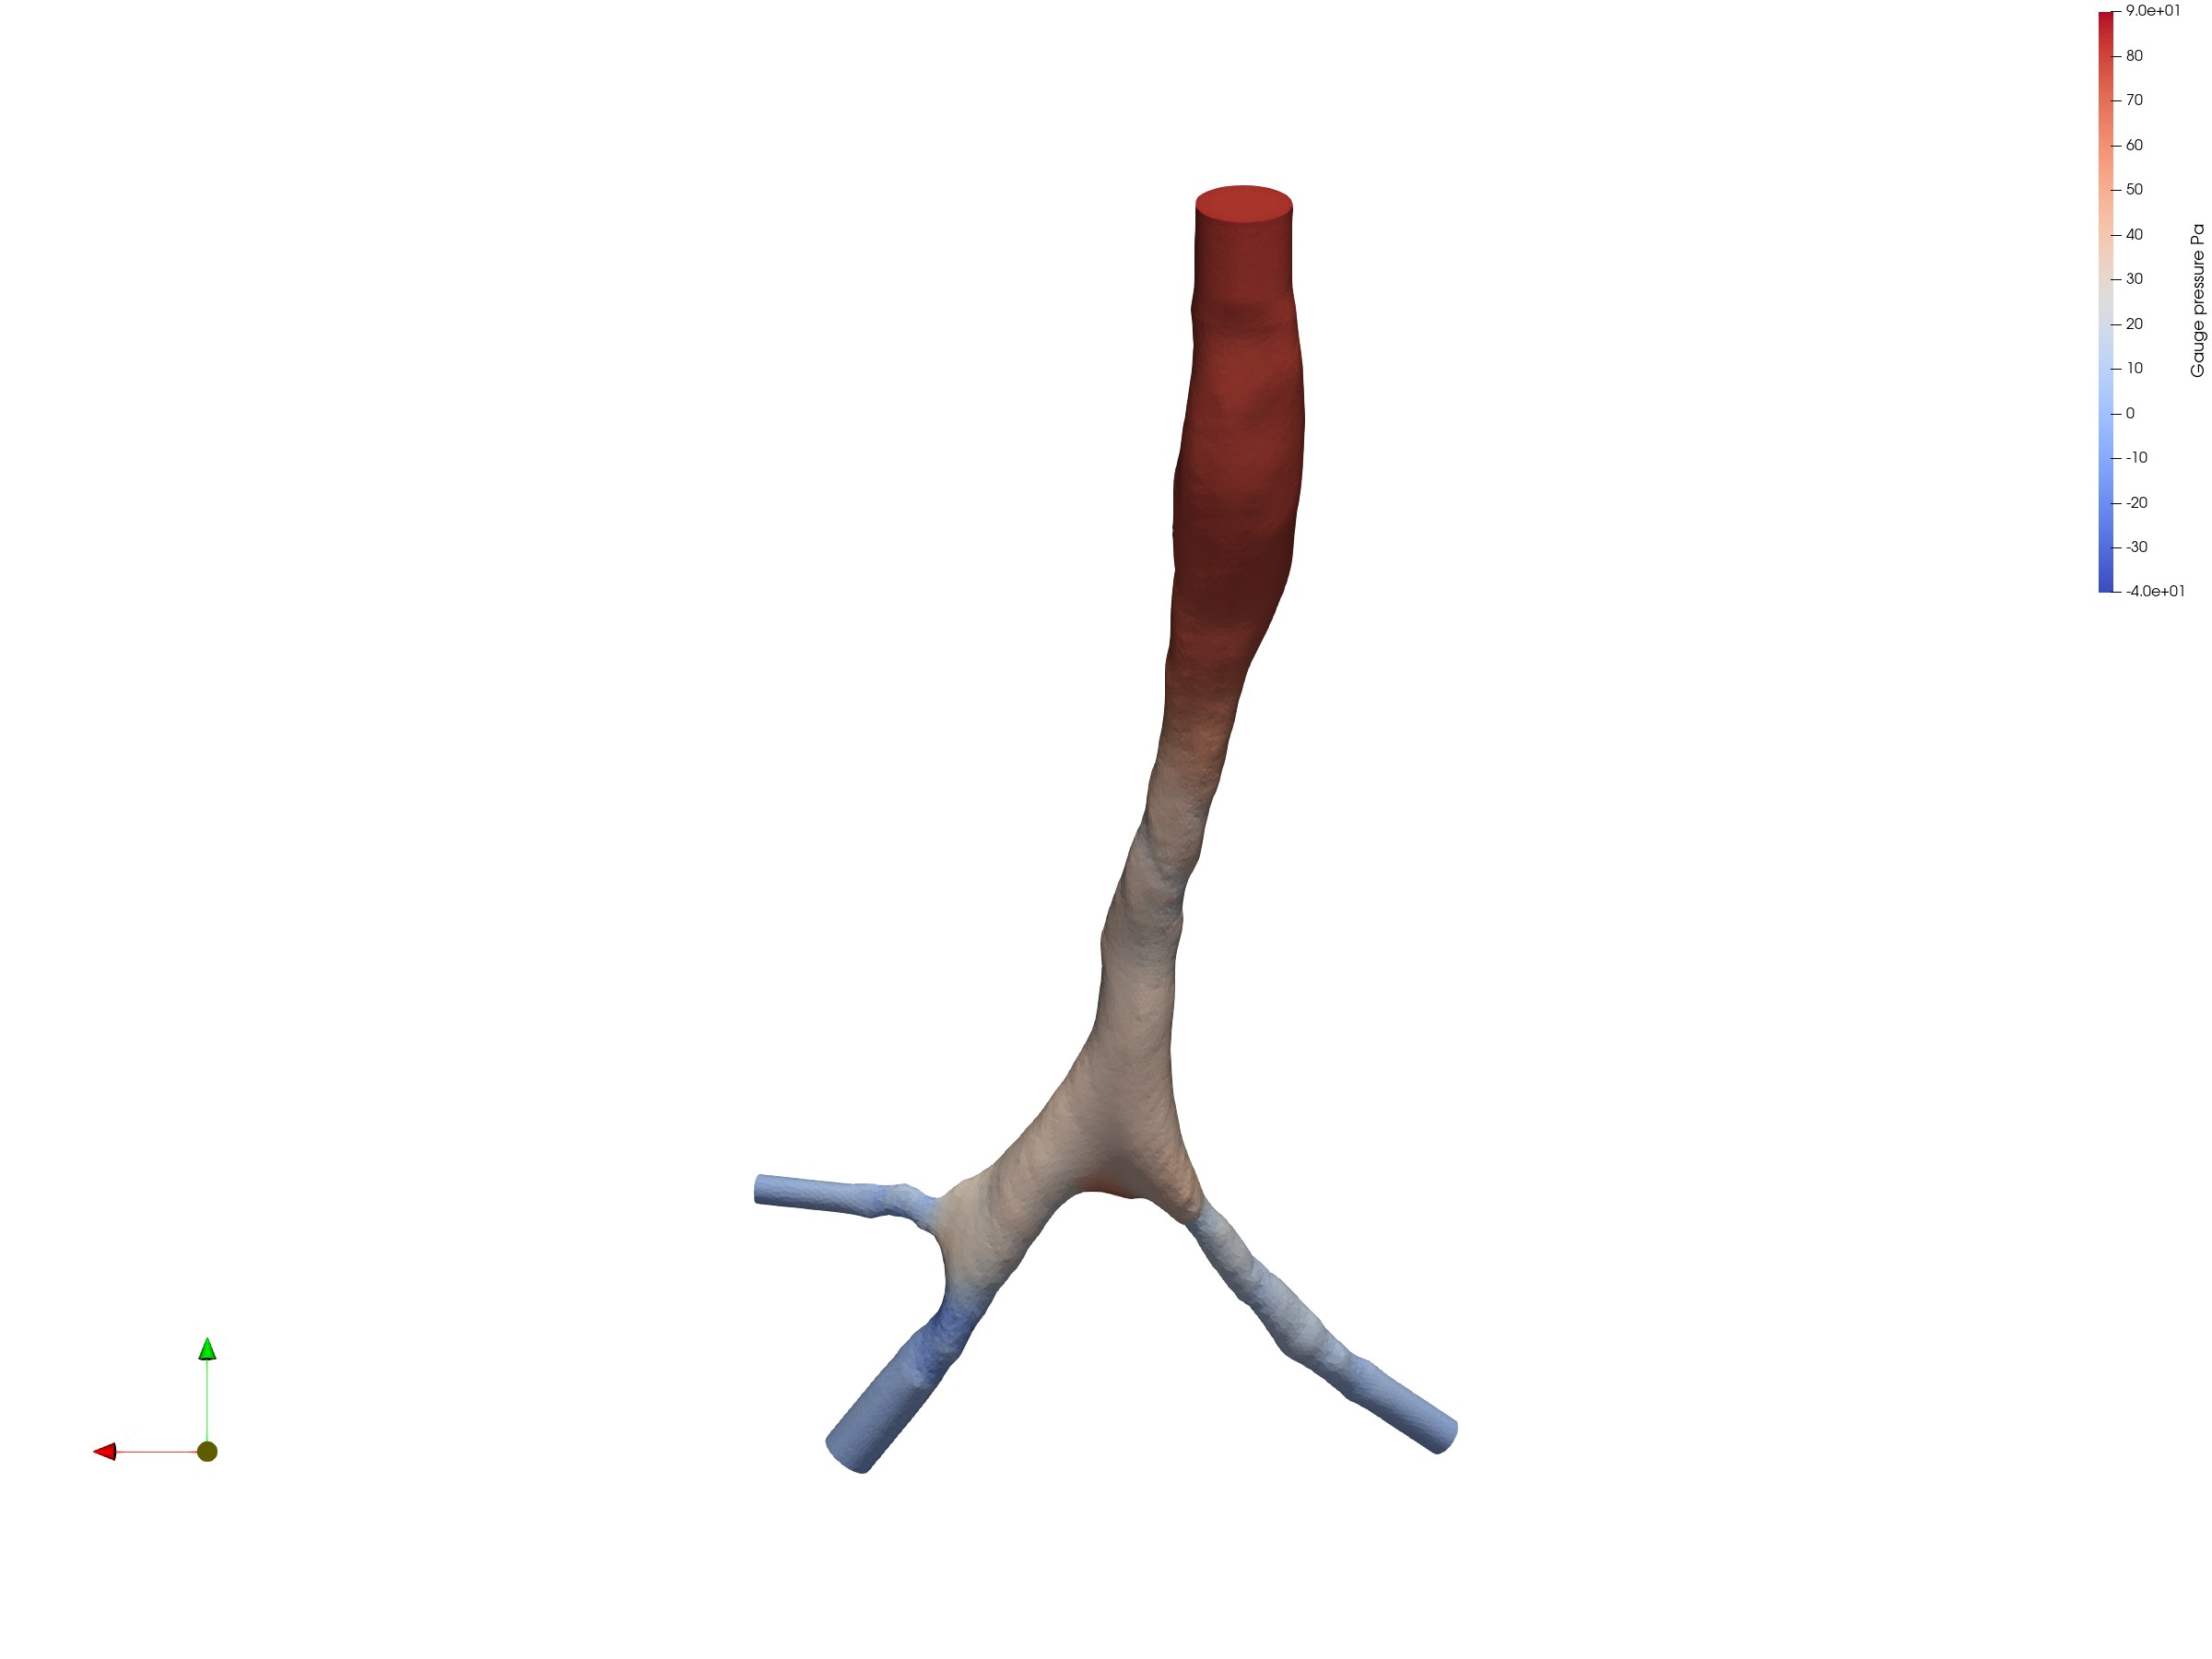
\includegraphics[width=0.92\textwidth]{assignment4_pressure_distribution.png}
  \caption{Postoperative dimensional gauge-pressure distribution at the
  converged steady solution (iteration 589), shown in anatomical frontal view.
  OpenFOAM kinematic pressure was multiplied by an air density of
  \SI{1.204}{\kilogram\per\metre\cubed}; outlet gauge pressure is zero.}
  \label{fig:pressure}
\end{figure}

\begin{figure}[htbp]
  \centering
  \resizebox{0.95\textwidth}{!}{% GNUPLOT: LaTeX picture with Postscript
\begingroup
  \makeatletter
  \providecommand\color[2][]{%
    \GenericError{(gnuplot) \space\space\space\@spaces}{%
      Package color not loaded in conjunction with
      terminal option `colourtext'%
    }{See the gnuplot documentation for explanation.%
    }{Either use 'blacktext' in gnuplot or load the package
      color.sty in LaTeX.}%
    \renewcommand\color[2][]{}%
  }%
  \providecommand\includegraphics[2][]{%
    \GenericError{(gnuplot) \space\space\space\@spaces}{%
      Package graphicx or graphics not loaded%
    }{See the gnuplot documentation for explanation.%
    }{The gnuplot epslatex terminal needs graphicx.sty or graphics.sty.}%
    \renewcommand\includegraphics[2][]{}%
  }%
  \providecommand\rotatebox[2]{#2}%
  \@ifundefined{ifGPcolor}{%
    \newif\ifGPcolor
    \GPcolortrue
  }{}%
  \@ifundefined{ifGPblacktext}{%
    \newif\ifGPblacktext
    \GPblacktexttrue
  }{}%
  % define a \g@addto@macro without @ in the name:
  \let\gplgaddtomacro\g@addto@macro
  % define empty templates for all commands taking text:
  \gdef\gplbacktext{}%
  \gdef\gplfronttext{}%
  \makeatother
  \ifGPblacktext
    % no textcolor at all
    \def\colorrgb#1{}%
    \def\colorgray#1{}%
  \else
    % gray or color?
    \ifGPcolor
      \def\colorrgb#1{\color[rgb]{#1}}%
      \def\colorgray#1{\color[gray]{#1}}%
      \expandafter\def\csname LTw\endcsname{\color{white}}%
      \expandafter\def\csname LTb\endcsname{\color{black}}%
      \expandafter\def\csname LTa\endcsname{\color{black}}%
      \expandafter\def\csname LT0\endcsname{\color[rgb]{1,0,0}}%
      \expandafter\def\csname LT1\endcsname{\color[rgb]{0,1,0}}%
      \expandafter\def\csname LT2\endcsname{\color[rgb]{0,0,1}}%
      \expandafter\def\csname LT3\endcsname{\color[rgb]{1,0,1}}%
      \expandafter\def\csname LT4\endcsname{\color[rgb]{0,1,1}}%
      \expandafter\def\csname LT5\endcsname{\color[rgb]{1,1,0}}%
      \expandafter\def\csname LT6\endcsname{\color[rgb]{0,0,0}}%
      \expandafter\def\csname LT7\endcsname{\color[rgb]{1,0.3,0}}%
      \expandafter\def\csname LT8\endcsname{\color[rgb]{0.5,0.5,0.5}}%
    \else
      % gray
      \def\colorrgb#1{\color{black}}%
      \def\colorgray#1{\color[gray]{#1}}%
      \expandafter\def\csname LTw\endcsname{\color{white}}%
      \expandafter\def\csname LTb\endcsname{\color{black}}%
      \expandafter\def\csname LTa\endcsname{\color{black}}%
      \expandafter\def\csname LT0\endcsname{\color{black}}%
      \expandafter\def\csname LT1\endcsname{\color{black}}%
      \expandafter\def\csname LT2\endcsname{\color{black}}%
      \expandafter\def\csname LT3\endcsname{\color{black}}%
      \expandafter\def\csname LT4\endcsname{\color{black}}%
      \expandafter\def\csname LT5\endcsname{\color{black}}%
      \expandafter\def\csname LT6\endcsname{\color{black}}%
      \expandafter\def\csname LT7\endcsname{\color{black}}%
      \expandafter\def\csname LT8\endcsname{\color{black}}%
    \fi
  \fi
    \setlength{\unitlength}{0.0500bp}%
    \ifx\gptboxheight\undefined%
      \newlength{\gptboxheight}%
      \newlength{\gptboxwidth}%
      \newsavebox{\gptboxtext}%
    \fi%
    \setlength{\fboxrule}{0.5pt}%
    \setlength{\fboxsep}{1pt}%
    \definecolor{tbcol}{rgb}{1,1,1}%
\begin{picture}(8500.00,4800.00)%
    \gplgaddtomacro\gplbacktext{%
      \csname LTb\endcsname%%
      \put(487,562){\makebox(0,0)[r]{\strut{}$30$}}%
      \csname LTb\endcsname%%
      \put(487,1024){\makebox(0,0)[r]{\strut{}$35$}}%
      \csname LTb\endcsname%%
      \put(487,1485){\makebox(0,0)[r]{\strut{}$40$}}%
      \csname LTb\endcsname%%
      \put(487,1946){\makebox(0,0)[r]{\strut{}$45$}}%
      \csname LTb\endcsname%%
      \put(487,2407){\makebox(0,0)[r]{\strut{}$50$}}%
      \csname LTb\endcsname%%
      \put(487,2868){\makebox(0,0)[r]{\strut{}$55$}}%
      \csname LTb\endcsname%%
      \put(487,3329){\makebox(0,0)[r]{\strut{}$60$}}%
      \csname LTb\endcsname%%
      \put(487,3791){\makebox(0,0)[r]{\strut{}$65$}}%
      \csname LTb\endcsname%%
      \put(487,4252){\makebox(0,0)[r]{\strut{}$70$}}%
      \csname LTb\endcsname%%
      \put(576,386){\makebox(0,0){\strut{}$0$}}%
      \csname LTb\endcsname%%
      \put(1667,386){\makebox(0,0){\strut{}$2$}}%
      \csname LTb\endcsname%%
      \put(2758,386){\makebox(0,0){\strut{}$4$}}%
      \csname LTb\endcsname%%
      \put(3849,386){\makebox(0,0){\strut{}$6$}}%
      \csname LTb\endcsname%%
      \put(4940,386){\makebox(0,0){\strut{}$8$}}%
      \csname LTb\endcsname%%
      \put(6031,386){\makebox(0,0){\strut{}$10$}}%
      \csname LTb\endcsname%%
      \put(7122,386){\makebox(0,0){\strut{}$12$}}%
      \csname LTb\endcsname%%
      \put(8212,386){\makebox(0,0){\strut{}$14$}}%
    }%
    \gplgaddtomacro\gplfronttext{%
      \csname LTb\endcsname%%
      \put(154,2407){\rotatebox{-270.00}{\makebox(0,0){\strut{}Area-interpolated centerline pressure (Pa)}}}%
      \csname LTb\endcsname%%
      \put(4394,123){\makebox(0,0){\strut{}Centerline distance from mapped superior limit (mm)}}%
      \csname LTb\endcsname%%
      \put(4394,4516){\makebox(0,0){\strut{}Postoperative pressure through the anatomically matched region}}%
    }%
    \gplbacktext
    \put(0,0){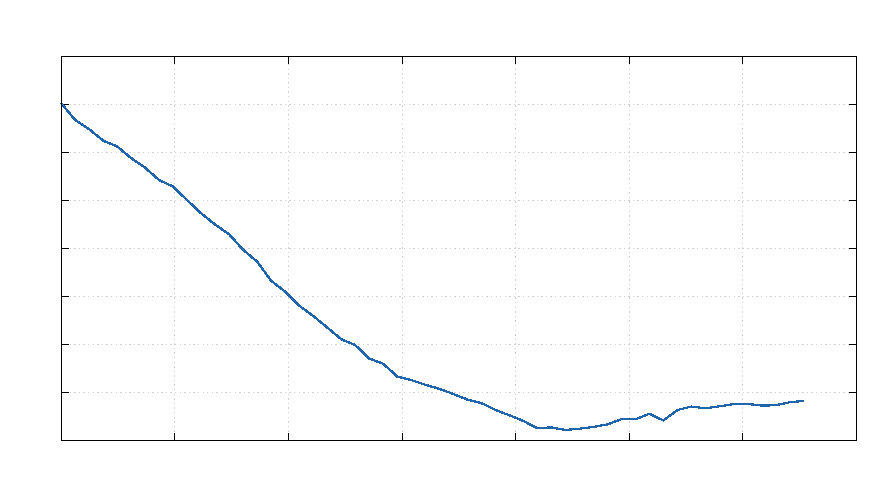
\includegraphics[width={425.00bp},height={240.00bp}]{figures/assignment4_centerline_pressure}}%
    \gplfronttext
  \end{picture}%
\endgroup
}
  \caption{Centerline-interpolated dimensional pressure across the postoperative
  region corresponding to the preoperative stenosis. Distance is measured from
  the mapped superior limit toward the mapped inferior limit. This profile shows
  local pressure evolution; resistance is calculated separately from
  area-averaged pressures on the bounding planes.}
  \label{fig:centerline_pressure}
\end{figure}

\subsection{Outlet and lung flow distribution}

Outlet flow was obtained by integrating outward-normal volumetric flux over each
patch. The right superior and inferior lobar outlets were grouped as the right
lung; the left main bronchus formed the left group. The primary left/right result
was

\begin{equation}
  Q_R = 73.17\%, \qquad Q_L = 26.83\%.
\end{equation}

The individual outlet values in Table~\ref{tab:outlet_flow} provide the supporting
lobar decomposition. Because identical zero gauge pressure was imposed at all
outlets, no 73/27 split was prescribed. The unequal distribution instead reflects
the geometric and hydraulic resistance of the branches resolved within the
truncated airway domain.

\begin{table}[htbp]
  \centering
  \caption{Outlet flow rates and fractions.}
  \label{tab:outlet_flow}
  \begin{tabular}{@{}lrrrr@{}}
    \toprule
    Case & Outlet 1 (\%) & Outlet 2 (\%) & Outlet 3 (\%) & Imbalance (\%) \\
    \midrule
    Postoperative & 11.23 & 61.94 & 26.83 & $6.0\times10^{-7}$ \\
    \bottomrule
  \end{tabular}
\end{table}

\begin{table}[htbp]
  \centering
  \caption{Postoperative left/right lung flow distribution.}
  \label{tab:lung_flow}
  \begin{tabular}{@{}lrr@{}}
    \toprule
    Lung & Flow rate (\si{\metre\cubed\per\second}) & Fraction (\%) \\
    \midrule
    Left  & $8.9449\times10^{-6}$ & 26.83 \\
    Right & $2.4388\times10^{-5}$ & 73.17 \\
    \bottomrule
  \end{tabular}
\end{table}

\subsection{Local resistance before the bifurcation}
\label{sec:steady_resistance}

Two planes normal to the centerline delimit a fixed section before the
bifurcation, corresponding approximately to the location of the preoperative
constriction. These same plane definitions are reused for every mesh and for the
transient Assignment 6 analysis. With dimensional pressure difference
$\Delta P$ and volumetric flow $Q$, local resistance is

\begin{equation}
  R(t)=\frac{\overline{P}_{\mathrm{up}}(t)-
  \overline{P}_{\mathrm{down}}(t)}{Q(t)}.
  \label{eq:local_resistance}
\end{equation}

For the incompressible OpenFOAM pressure field $p$,
$\Delta P=\rho\,\Delta p$. Area-averaged kinematic pressures were
\SI{53.70}{\metre\squared\per\second\squared} upstream and
\SI{27.99}{\metre\squared\per\second\squared} downstream. With
$\rho=\SI{1.204}{\kilogram\per\metre\cubed}$, the local pressure drop was
\SI{30.95}{\pascal}; at $Q=\SI{3.347e-5}{\metre\cubed\per\second}$ this gives
$R=\SI{9.25e5}{\pascal\second\per\metre\cubed}$, equivalent to
\SI{15.41}{\pascal\per\litre\per\minute}. The matched-plane mean axial and peak
velocities were \SI{6.53}{\metre\per\second} and
\SI{9.25}{\metre\per\second}, respectively.

\begin{figure}[htbp]
  \centering
  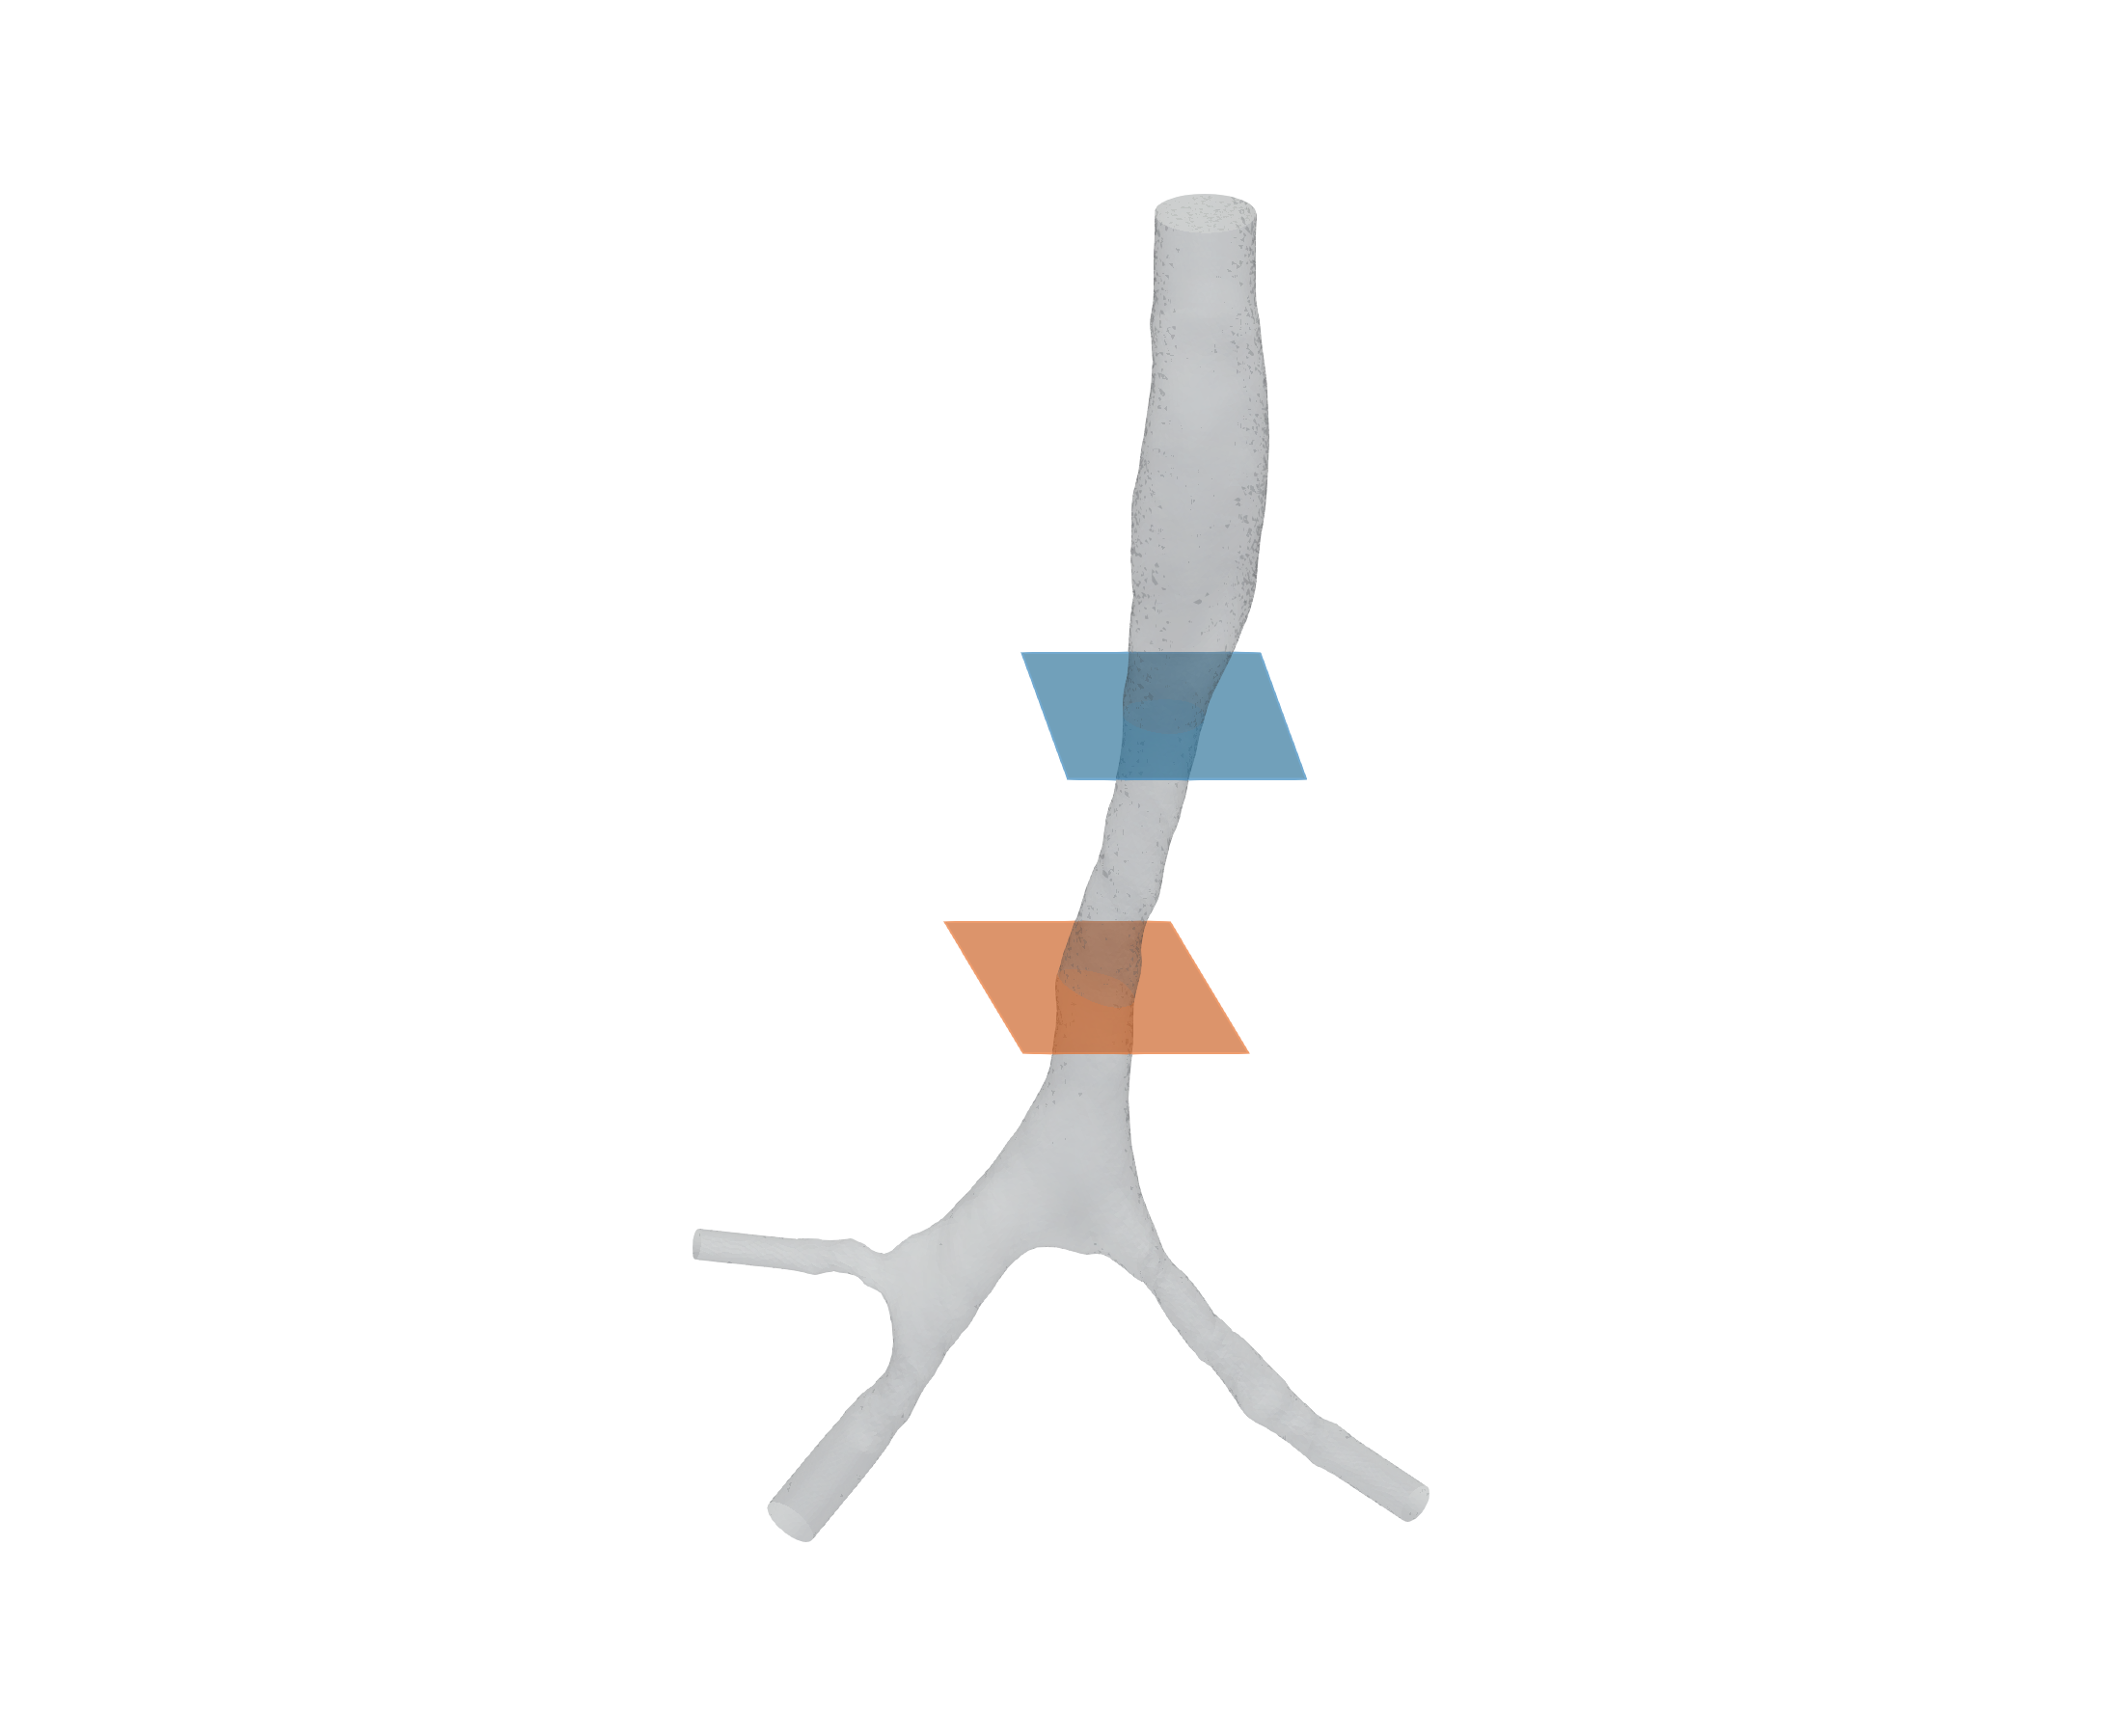
\includegraphics[width=0.76\textwidth]{assignment4_resistance_planes.png}
  \caption{Fixed centerline-normal planes delimiting the postoperative matched
  tracheal region. The blue superior plane is the upstream pressure section and
  the orange inferior plane is the downstream section. Their origins and normals
  are archived in a versioned JSON definition and reused unchanged for steady,
  mesh-sensitivity, and transient analyses.}
  \label{fig:resistance_section}
\end{figure}

\begin{table}[htbp]
  \centering
  \caption{Steady postoperative local-resistance calculation.}
  \label{tab:steady_resistance}
  \begin{tabular}{@{}lr@{}}
    \toprule
    Quantity & Value \\
    \midrule
    Upstream area-averaged kinematic pressure & 53.695 \si{\metre\squared\per\second\squared} \\
    Downstream area-averaged kinematic pressure & 27.993 \si{\metre\squared\per\second\squared} \\
    Pressure difference $\Delta P$ & 30.945 \si{\pascal} \\
    Volumetric flow $Q$ & \num{3.347e-5} \si{\metre\cubed\per\second} \\
    Resistance $R=\Delta P/Q$ & \num{9.247e5} \si{\pascal\second\per\metre\cubed} \\
    \bottomrule
  \end{tabular}
\end{table}

% -----------------------------------------------------------------------------
\section{Transient postoperative analysis}
\label{sec:transient_results}

\subsection{Time-step convergence}

At the time of report assembly, the full \SI{2}{\second} calculation on the
selected \num{0.15}~mm HXT mesh was running on 48 MPI ranks. Startup tests showed
that adaptive stepping maintained the maximum Courant number close to the target
of 2 while the mean remained substantially lower. Final linear-solver residuals
were typically of order $10^{-9}$ and final global continuity errors of order
$10^{-12}$. Some startup steps did not satisfy the configured outer PIMPLE
criterion within three correctors. The final log must therefore be parsed before
claiming complete time-step convergence or periodicity; no incomplete transient
quantity is substituted by extrapolation.

\begin{figure}[htbp]
  \centering
  \fbox{\parbox[c][5.5cm][c]{0.88\textwidth}{\centering
    Placeholder: transient residuals and convergence status per time step}}
  \caption{Residual evolution for the postoperative transient simulation.
  Highlight any time steps that did not satisfy the selected criterion.}
  \label{fig:transient_residuals}
\end{figure}

\subsection{Velocity vectors at representative phases}

Select three time points from the imposed breathing waveform, for example
acceleration, peak inspiratory flow, and deceleration or flow reversal. The
exact selection must be justified from the waveform rather than chosen only for
visual appearance.

\begin{figure}[htbp]
  \centering
  \fbox{\parbox[c][6.5cm][c]{0.88\textwidth}{\centering
    Placeholder: velocity vectors coloured by magnitude at three relevant time
    points using a common colour scale}}
  \caption{Postoperative transient velocity vectors at three phases of the
  breathing cycle. State each time and inlet flow rate.}
  \label{fig:transient_vectors}
\end{figure}

\subsection{Breathing waveform and time-varying resistance}

The applied inlet flow rate and the local resistance from
Equation~\ref{eq:local_resistance} are evaluated over one complete breathing
cycle. The computational postoperative resistance is compared with the
constant-diameter expectation and with a qualitative preoperative sketch.

\begin{figure}[htbp]
  \centering
  \fbox{\parbox[c][7cm][c]{0.88\textwidth}{\centering
    Placeholder: (A) applied breathing flow waveform; (B) computed postoperative
    local resistance; (C) qualitative preoperative/postoperative resistance
    comparison}}
  \caption{Breathing-cycle flow rate and local resistance. Resistance near zero
  flow must be handled carefully because direct division by $Q(t)$ becomes
  ill-conditioned.}
  \label{fig:transient_resistance}
\end{figure}

% -----------------------------------------------------------------------------
\section{Discussion}
\label{sec:discussion}

\subsection{Interpretation of outlet conditions and lung-flow split}

Applying the same static pressure at every distal outlet deliberately leaves the
left/right flow division unconstrained, making it an output of the reconstructed
geometry rather than an imposed boundary-condition ratio. The predicted
73.17\% right and 26.83\% left distribution is therefore a defensible measure of
the relative aerodynamic resistance of the resolved postoperative branches.
Differences in calibre, pathway length, branching angle, curvature, and local
flow separation can all contribute to the unequal result.

This distribution should not, however, be interpreted as the child's measured
physiological lung ventilation. The model ends at truncated bronchial outlets and
therefore excludes the resistance of unresolved peripheral airways and the
compliance of the distal lungs. A more physiologically detailed extension could
apply distal resistance conditions such as

\begin{equation}
  P_i = P_{\mathrm{alv}} + R_i Q_i,
\end{equation}

or coupled resistance--compliance outlet models. Such conditions would preserve
an emergent flow split while representing peripheral lung mechanics, provided
that patient-specific parameters were available.

\subsection{Mesh sensitivity and optimal mesh}

Resistance and the small right-superior branch split were more mesh-sensitive
than total right-lung fraction. From 0.15 to 0.12 mm, all selected metrics changed
by at most 2.02\%, while cell count increased by 92\% and solver execution time
by 157\%. The 0.12 mm case also failed residual control at 2000 iterations,
whereas 0.15 mm converged in 1611. With a practical 2.5\% acceptance threshold,
the 0.15 mm mesh is selected as the optimal balance between apparent spatial
convergence and computational efficiency.

\subsection{Constant-diameter resistance during inspiration}

For fully developed laminar flow in a rigid constant-diameter tube,
Poiseuille's law gives $\Delta P=128\mu LQ/(\pi D^4)=RQ$. Geometry and fluid
properties are constant, so increasing inspiratory flow produces a proportional
pressure drop while $R=\Delta P/Q$ remains constant. Patient-specific curvature,
developing flow, bifurcation, separation, and inertial losses can instead make
pressure drop nonlinear in flow. Transient inertia can also create phase
differences between pressure and flow, so instantaneous resistance need not
remain constant.

\subsection{Limitations}

Potential limitations include:

\begin{itemize}
  \item static CT geometry despite the dynamic nature of tracheomalacia;
  \item rigid airway walls and absence of fluid--structure interaction;
  \item steady inlet flow instead of a respiratory waveform;
  \item idealised outlet pressure conditions;
  \item uncertainty from segmentation and clipping-point placement;
  \item an isotropic first-order tetrahedral mesh without dedicated prism
        boundary layers;
  \item the selected laminar-flow assumption; and
  \item analysis of a limited number of anatomical cases.
\end{itemize}

With additional resources, refinement should focus locally on the matched
tracheal region, carina, and small right-superior branch rather than reducing
global size uniformly. All cases should first meet residual and monitored-integral
criteria. Additional levels around the apparent asymptotic range, consistently
generated prism layers, Richardson extrapolation, and a grid-convergence index
would strengthen numerical uncertainty estimates. Runtime, memory, mesh quality,
and section-area variation should be tracked alongside each physical metric.

\subsection{Handling transient non-convergence}

[Identify unconverged time steps and discuss targeted remedies: reduce the time
step, constrain the Courant number, increase inner iterations/correctors,
improve mesh quality, use a better initial condition from a previous cycle, and
simulate additional cycles until periodic behaviour is obtained. Report which
changes would be tested first and why.]

% -----------------------------------------------------------------------------
\section{Conclusions}
\label{sec:conclusions}

[Summarise the principal quantitative findings, state whether the intervention
improved the simulated flow characteristics, and report whether the conclusions
were robust to mesh refinement.]

% -----------------------------------------------------------------------------
\section*{Reproducibility statement}
\addcontentsline{toc}{section}{Reproducibility statement}

The complete workflow is documented in \texttt{WORKFLOW.md}. Record the Git
commit, Slicer version, Gmsh version, OpenFOAM image identifier, mesh sizes,
cell counts, and solver settings used for the final results. The scripts
\texttt{create\_volume\_mesh.sh}, \texttt{run\_cfd.sh},
\texttt{run\_fine\_cfd.sh}, and \texttt{fetch\_cfd\_results.sh} automate the
meshing, remote execution, reconstruction, and retrieval stages.

% -----------------------------------------------------------------------------
% References
% -----------------------------------------------------------------------------
\begin{thebibliography}{9}

\bibitem{taherian2017}
S.~Taherian, H.~Rahai, B.~Gomez, T.~Waddington, and F.~Mazdisnian,
``Computational fluid dynamics evaluation of excessive dynamic airway
collapse,''
\textit{Clinical Biomechanics}, vol.~50, pp.~145--153, 2017.
\url{https://doi.org/10.1016/j.clinbiomech.2017.10.018}.

\bibitem{arcieri2018}
L.~Arcieri, V.~Pak, V.~Poli, R.~Baggi, P.~Serio, N.~Assanta, R.~Moschetti,
B.~Noccioli, S.~De Masi, L.~Mirabile, and B.~Murzi,
``Tracheal surgery in children: outcome of a 12-year survey,''
\textit{Interactive CardioVascular and Thoracic Surgery}, vol.~26, no.~4,
pp.~660--666, 2018.

\bibitem{openfoam}
OpenCFD Ltd.,
\textit{OpenFOAM User Guide},
\url{https://www.openfoam.com/documentation/}.

\bibitem{gmsh}
C.~Geuzaine and J.-F.~Remacle,
``Gmsh: A three-dimensional finite element mesh generator with built-in pre-
and post-processing facilities,''
\textit{International Journal for Numerical Methods in Engineering},
vol.~79, no.~11, pp.~1309--1331, 2009.

\bibitem{slicer}
A.~Fedorov et al.,
``3D Slicer as an image computing platform for the Quantitative Imaging
Network,''
\textit{Magnetic Resonance Imaging}, vol.~30, no.~9, pp.~1323--1341, 2012.

\bibitem{vmtk}
L.~Antiga et al.,
``An image-based modeling framework for patient-specific computational
hemodynamics,''
\textit{Medical \& Biological Engineering \& Computing}, vol.~46,
pp.~1097--1112, 2008.

\end{thebibliography}

\end{document}
